% simple.tex

\documentclass{article}[12pt,a4paper]

\usepackage{hyperref}
\hypersetup{
    colorlinks,
    citecolor=black,
    filecolor=black,
    linkcolor=black,
    urlcolor=black
}

\usepackage{listings}
\usepackage{color}
\usepackage{longtable}
\usepackage{enumitem}
\usepackage{subfigure}
\usepackage{graphicx}
\usepackage{hyperref}
\usepackage{bookmark}
\usepackage{framed}
\usepackage{fontspec}
\usepackage{parskip}

\newfontfamily\raleway{Raleway}

\graphicspath{ {images/} }

\definecolor{codegreen}{rgb}{0,0.6,0}
\definecolor{codegray}{rgb}{0.5,0.5,0.5}
\definecolor{codepurple}{rgb}{0.58,0,0.82}
\definecolor{backcolour}{rgb}{0.95,0.95,0.92}
\definecolor{uigreen}{RGB}{82,170,94}
\definecolor{uiyellow}{RGB}{240,173,78}
\definecolor{uiblue}{RGB}{91,192,222}

\definecolor{lightgray}{rgb}{.9,.9,.9}
\definecolor{darkgray}{rgb}{.4,.4,.4}
\definecolor{purple}{rgb}{0.65, 0.12, 0.82}

\lstdefinelanguage{JavaScript}{
  keywords={typeof, new, true, false, catch, function, return, null, catch, switch, var, if, in, while, do, else, case, break},
  keywordstyle=\color{blue}\bfseries,
  ndkeywords={class, export, boolean, throw, implements, import, this},
  ndkeywordstyle=\color{darkgray}\bfseries,
  identifierstyle=\color{black},
  sensitive=false,
  comment=[l]{//},
  morecomment=[s]{/*}{*/},
  commentstyle=\color{purple}\ttfamily,
  stringstyle=\color{red}\ttfamily,
  morestring=[b]',
  morestring=[b]"
}

\lstset{
   language=JavaScript,
   backgroundcolor=\color{lightgray},
   extendedchars=true,
   basicstyle=\footnotesize\ttfamily,
   showstringspaces=false,
   showspaces=false,
   numbers=left,
   numberstyle=\footnotesize,
   numbersep=9pt,
   tabsize=2,
   breaklines=true,
   showtabs=false,
   captionpos=b
}

\lstdefinestyle{python}{
    backgroundcolor=\color{backcolour},   
    commentstyle=\color{codegreen},
    keywordstyle=\color{magenta},
    numberstyle=\tiny\color{codegray},
    stringstyle=\color{codepurple},
    basicstyle=\footnotesize,
    breakatwhitespace=false,         
    breaklines=true,                 
    captionpos=b,                    
    keepspaces=true,                 
    numbers=left,                    
    numbersep=5pt,                  
    showspaces=false,                
    showstringspaces=false,
    showtabs=false,                  
    tabsize=2
}

\begin{document}

\title{WJEC GCE Computing CG2 - Extended Task}

\author{Candidate Name: Daniel Roberts\\
        Candidate Number: 4699\\
        Centre Name: Shrewsbury Sixth Form College\\
        Centre Number: 29285}

\date{}

\maketitle

\tableofcontents

\cleardoublepage

\part{Analysis and Design}
This part of documentation contains the analysis that was performed on Parkwood Vale Harriers, taking into account what the running club asked for in their brief, and exploring these requirements. It also covers preliminary designs that were created for the system, including interface designs for every page, design of data structures and process design, details of the different algorithms that have been used, and information on how the system interacts with different aspects of itself; ie. the different technologies that have been used.

\section{Problem Definition}
\subsection{Background}
Parkwood Vale Harriers is a running club that serves the fitness needs of many different members, through both regular meetup sessions, and races. The club gets involved in the local community, a position that consists, in part, of raising money for local charities.

Recently, the club has decided to raise money for one of charities by putting on a relay event, wherein a team of runners will run, non-stop, from John O\textsc{\char13} Groats to Land’s End, in the shortest time possible. The team will consist of eight members, and each runner will run for an hour at a time, whilst the others rest in minibus. The entire trip is estimated to take three days and as a result of this, each member of team will have to be very fit.

In order to increase their chances of completing run, the club has decided to find out the most appropriate team, based on results of a physically challenging programme. This programme will consist of running, cycling and swimming, and will serve to ensure that only the very best members of the club are included in the team.

\subsection{Broad Aims}
The running club has commissioned  a computer based system that will allow runners to keep an accurate record of their running, cycling and swimming sessions. This data will then be used to calculate an informed decision of the most appropriate team for the relay race.

The system must allow each runner to monitor their progress during programme, clearly showing them the extent to which they have improved. As such, the system must provide an interface to allow runner to add each session they perform, with spaces for type of training, time spent, how hard they pushed themselves, and other such parameters. Using this data, the system must then calculate number of calories burned in the session, providing a series of data points through which performance of the runner can be monitored.

To further aid in this, the system must be able to output these sessions in a clear format that the runner is able to clearly understand. This can be achieved through the use of tables to display each session in a listed, tabular format, as well as through graphs and charts to display data in a graphical form; this makes overall performance trends easy to visualise.

Due to the nature of the system, the ability to store certain personal information, such as name, age and weight of runner, must also be included. The runner should have ability to input this information themselves, most likely upon first use of the system. There should be the ability to modify this data, in result of an error being made or the circumstances of the runner changing.

An important aspect of the system, and one that is key to promoting the competitive values of club, is the ability to compare results with other participants in program. This area of the system should allow the runners to compare key aspects of their performance, such as the results of their individual sessions, as well as their overall performance over time in all three of the activities.

As the main point of the system, the ability to select final team must also be included. By analysing data points provided by runners, the system should be able to choose most appropriate team.

\subsection{Limitations}
Though the brief provided by running club contains several good ideas and acts as an effective base upon which to work, there are a number of areas which the running club has not thought about that could be factored into solution, thus creating a more effective and, over all, higher quality system. 

One very important factor that the running club has left out is security. In a system like this, where intensely personal data is being stored, including data that runner may not which to become public, such as their weight, it is important that the data is stored in a secure manner that allows only those with correct permissions to access it. 

Another issue with the brief is that of an objective decision being made when selecting the team. Running a marathon is about far more than just physical fitness; more personal aspects, such as how well runners get along, as well as different roles within team, should also be taken into account for maximum efficiency. The system would be unable to do this (without each runner giving their opinion on others, which is unrealistic), and so the team it comes up with may not be most appropriate choice. 

Another limitation in the system is that data will have to be entered manually: there is no way of extrapolating data from some sort of personal tracking device without diverging some distance away from the actual brief. This could result in some issues with accuracy, or even with malpractice: people could enter exaggerated data in order to manipulate the rankings and make themselves appear more suitable for the team. A mixture of validation and verification can be put in place to prevent this, such as ensuring users cannot go for a straight eight hour swim (something which is obviously unrealistic), but this will be unable to catch all cases of exaggeration; it is therefore necessary to rely on the goodwill and sportsmanship of runners.

Furthermore, the system relies on the premise that runners will add every session they perform to the application. It is not unlikely that they will go on unsolicited sessions that they do not bother adding, or they may simply forget. There is no foolproof manner to prevent these occurences, but a number of steps can be taken to reduce their likelihood, such as by making the process of adding a session as simple as possible - it follows that the easier the process is, the more likely the runners are to do it.

In addition, the brief asks for only the top eight members of the running team to be calculated. This does not take into account the possibility of injuries or runners dropping out for other reasons; as such, the system should also calculate a number of reserve runners, in the event of an accident.

Additionally, the system will need a team of experienced professionals to keep and maintain it - the running club may wish for an aspect of the system to be modified, and, depending on its complexity, this could require great expertise.

Though pains will be taken to ensure that the system is easy to use, it will still require a degree of training for those members of the club who lack experience in using computers; this will take time, something that, with the charity event looming, the running club may not have.

\subsection{Assumptions}
Throughout the system, a number of assumptions have been made in order to increase ease of development. 

One of these is that in each individual session, only one method of exercise will be used, such as breaststroke for an entire swimming session or a leisurely speed for an entire cycling session. Though this is alleviated to some extent by the ability to add multiple sessions for each sport on a single day, the assumption still has to be made. 

In addition to this, an assumption that each session lasts for at least an hour has been made: the time picker uses stages of sixty minutes, as opposed to thirty or fifteen.

Naturally, the system also assumes that the runner is relatively proficient with a computer based interface. Effort has been put in to make the system as runner friendly and as easy to use as possible, but someone using a computer for first time will undoubtedly find it more difficult than someone with a little experience.

\subsection{Objectives}
In order for the system to be of an acceptable quality, a number of objectives will have to be fulfilled. The system must:

\begin{itemize}
    \item Have a simple, clear interface that allows tasks to be performed easily. This will be done by using a consistent colour scheme for each of the sports - green for running, yellow for cycling and blue for swimming, as well as through the use of common runner interface paradigms such as buttons and dropdown boxes; these are all things that the runner should be familiar with, so they will find less difficulty in using the system. Additionally, animation will be used to transition smoothly from element to element, creating a more enjoyable runner experience that encourages the runner to use the system more frequently.

    \item Allow the runner to add, view, update and, if they choose, delete their personal information, including their name, email address, date of birth and phone number. For this to be achieved, a database will have to be designed and built with appropriate columns and data types, and pages and routes will have to be designed and programmed to facilitate the adding, viewing and deleting of this data - a registration page could be used for adding the data, and a profile page for viewing, updating and deleting the data.

    \item Allow the runner to add, view and delete the training sessions they perform in over course of period; this will include information like date and time of the session, the speed they were at, and how well it went. To do this, a database table will have to be designed and built in order to store these activities, and pages will have to be designed and built to facilitate the adding, viewing and deleting of the training sessions. Processes and routes will also have to be built in order to make these functions actually work.

    \item Ensure security of this data by giving each runner their own personal account, protected by a username and an encrypted password. To do this, an additional column in the users table will have to be built that stores the encrypted version of the password. Additionally, it will have to be decided which areas of the system can be accessed by those without an account.

    \item Calculate the number of calories burned in each session, by taking into account the runner's weight, time spent on the session,  the nature of the session, and how well the runner believed it went.

    \item Allow the runner to view graphical, interactive graphs of their sessions, allowing them to easily view trends in their performance.
\end{itemize}

\subsection{Justification of Proposed Solution}
When building a solution to a problem like one faced by Parkwood Vale Harriers, there are generally two methods available: utilising features of an existing software package, such as Microsoft Office Access, or programming an existing solution in a programming language, such as Visual Basic or Python. Both have their advantages and drawbacks: by utilising an existing package, much of system will already be developed; it only remains to manipulate system to meet needs of brief; but, on other hand, one can be limited by restrictions of software package, perhaps preventing final solution being as capable as it might otherwise have been.

An original solution created using a programming language would suffer from rather opposite issues: as a result of practically endless results that can be achieved through their use, there is a definite learning curve that is not present (or is less exacerbated) in software packages; as a result of this, development time will likely be considerably longer. Despite these drawbacks, it is clear that, if a programming language is used, final solution is likely to be of a higher quality: not only can more advanced features be implemented, these features - as well as those of a more basic level - are likely to be of a higher quality.  In addition, developer will have a greater understanding of system, as they will have built it entirely themselves (aside from any additional packages/libraries used); this will aid in areas like debugging, and will also make it easier to write up system documentation and like.

The question then falls to exactly which programming language is most appropriate. There are a large number of languages available, ranging from \textit{compiled} languages like Java, C\# and Visual Basic to \textit{interpreted} languages like Ruby, Python and PHP. differences between compiled and iterpreted languages are complex and varied, but, in essence, compiled languages are likely to perform algorithms more quickly (due to directly using native code of target machine), whereas code written in an interpreted language can be executed ``on the fly'', so to speak, increasing development speed. 

Python has an extremely wide range of benefits, perhaps more so than any other language, that make it absolutely suited to the needs of the running club. One of the benefits of Python is that it, not only can it connect to a database, it can also be used with any database system. This allows a great deal of freedom when choosing a database system - one can choose between MySQL, or SQLite, or even PostgreSQL. A database is the best method of storing the data, as it can be seperated into a number of logical tables, ensuring that the data is organised. Additionally, a database means that primary and foreign keys can be used, linking data tables and ensuring that each record is uniquely identifiable.

Python is also extremely simple to use - it is commonly ranked as the easisest language to learn, owing to its well thoght and structure and similarity, in many regards, to the English language. Indeed, when compared to a language like, say, Visual Basic, Python stands out as a bastion of sensible language design, and most importantly, common sense. This means that devlopment time can either be dramatically reduced, or 

However, this simplicity should not be mistaken for a lack of functionality: Python is an extremely capable languages; it can be used for everything from system administration to game design to, as in the case of this system, web development.

In order to persistently store runner's data, a database is needed. As is custom with applications of this sort, there will be one single database file, within which will be a number of tables. The system will also make use of a number of arrays and JSON structures, to temporarily store data.

Additionally, Python, combined with HTML and CSS to create a web interface allows for a highly complex, fully interactive user interface to be created. Due to the nature of the languages, rapid prototyping can be achieved - any changes made are visible instantly, without the need for recompilation; this means that it is easier, as well as quicker, to create an appealing interface.

Common UI paradigms, such as buttons and input boxes can be included; these are effective, as the runner is likely to already have a working knowledge of how to use this system. 

\section{Database Tables}
The system will use SQLite database system. SQLite is a very popular database system (in same vein as MySQL). All of the database tables will be accessed sequentially - every item is ordered according to their primary key, which, as is custom for an SQLite database, is always an id number stored as an integer.

All of the fields will be of \textbf{variable} length: this is because the data will need to be shown back to the the user at different points throughout the system, something that, due to truncation, fixed length fields would make difficult. Additionally, this method is more space efficient.

Both tables will be accessed serially, because the order of the data does not matter - as primary keys are included on each record, they can be looked up this way.

\textbf{\textit{A note on validation: }}\textit{SQLite does not perform any validation itself. All validation will be performed during processing of data, before it is added into database. As such, details on validation performed on data saved to these tables can be found in their relevant section.}

\subsection{Users Table}
This table will store personal information for each runner. Whenever a runner creates an account, the data they input into registration form will end up in this table.

\begin{table}[htbp]
\begin{tabular}{|l|l|l|l|l|}
\hline
\textbf{Field Name}     & \textbf{Primary Key} & \textbf{Typical Data} & \textbf{Data Type} \\ \hline
id             & True        & 01                   & Integer   \\ \hline
name           & n/a         & John Smith           & String    \\ \hline
email          & n/a         & john@smith.com       & String    \\ \hline
username       & n/a         & john5                & String    \\ \hline
password\_hash & n/a         & pbkdf2:sha1:1000\$02 & String    \\ \hline
dob            & n/a         & 1997-02-02           & Date      \\ \hline
phone          & n/a         & 07722895880          & String    \\ \hline
weight         & n/a         & 74                   & Integer   \\ \hline
distance       & n/a         & less than 1          & String    \\ \hline
joined         & n/a         & 2015-01-04           & Date      \\ \hline
charity\_event & n/a         & True                 & Boolean   \\ \hline
\end{tabular}
\caption{Users Table}
\end{table}

\noindent
Each runner will be given an id which serves as their primary key; it is automatically incremented whenever a new runner is added, hence the data type of integer. 

The name will be used as an identifier throughout the system; as a string of characters, it has been given the string data type. Likewise with the email field: it can contain a combination of letters, numbers and other characters, and so has been will be set as a string. Username field will be a combination of the runner's first name and a random number; as such it will be a string. Password hash field stores an encrypted version of the runner's password; depending on the length of password, it can contain a very large number of letters, numbers and symbols - it is therefore a string. DOB field will store the runner's date of birth; the most appropriate data type would therefore be date; likewise with the date runner joined the application. No calculations are being performed on the runner's phone number, so it is more efficient to store it as a string - one character takes just 1 bit. Conversely, calculations will performed with runner's weight, so it is appropriate to store it as an integer. The charity event field stores either True or False depending on whether the runner wishes to be chosen to run in charity event; the most appropriate data type is therefore Boolean.

\subsection{Activities Table}

Every activity that the runners add will be given its own record in this table. Like the Users table, it is accessed serially - each new record is appended to the bottom. This is for the same reasons as above: the order in which the record is stored makes no difference, because they can be easily queried through their primary key. In addition, each activity will be linked to a runner through a foreign key, called user\_id; the relationsip is one-to-many in nature.

\begin{table}[h]
\begin{tabular}{|l|l|l|l|l|}
\hline
\textbf{Field Name} & \textbf{PK / FK} & \textbf{Typical Data} & \textbf{Data Type} & \textbf{Validation} \\ \hline
id                  & Primary          & 01                    & Integer  & Presence                      \\ \hline
sport               & n/a              & running               & String   & Presence                      \\ \hline
effigy              & n/a              & 5 mph                 & String   & Presence                      \\ \hline
date                & n/a              & 2015-01-04            & Date     & Presence, Range               \\ \hline
start               & n/a              & 8:00AM                & String   & Presence, Range               \\ \hline
finish              & n/a              & 10:00AM               & String   & Presence, Range               \\ \hline
hours               & n/a              & 2                     & Integer  & Presence                      \\ \hline
opinion             & n/a              & Brilliant             & String   & Presence                      \\ \hline
thoughts            & n/a              & It was great.         & String   & None                          \\ \hline
user\_id            & Foreign          & 02                    & Integer  & Presence                      \\ \hline
\end{tabular}
\caption{Activities Table}
\end{table}

\noindent
The id of each activity serves as its primary key; it is automatically incremented whenever a new activity is added, hence data type of integer. The sport field will be a string; it will store type of sport that activity belongs to, and so string is the most appropriate data type. The effigy field will store specific detail for each activity, such as speed for running sessions, or the type of stroke for swimming sessions. Due to wide the range of options that can be stored in this, and the fact that no calculations will be performed, the string data type would be the most appropriate. 

\section{User Interface Design}
The system will use a web based, graphical user interface. It will be simple and easy to use, making use of interface paradigms well known to the runners, such as buttons, form inputs and drop-down boxes, through their use of other computer systems. In order to increase usability, the system will make use of a consistent colour palette - each sport will be associated with a particular colour:\\

\begin{itemize}[label={}]
  \item \raleway{\textcolor{uigreen}{Green - rgb(82, 170, 94) - associated with running}}
  \item \textcolor{uiyellow}{Yellow - rgb(240, 173, 78) - associated with cycling}
  \item \textcolor{uiblue}{Blue - rgb(91, 192, 222) - associated with swimming}\\
\end{itemize}

\noindent
In addition, the system will use a consistent font throughout: Raleway, and its variants. Distinctive yet readable, Raleway is a highly renowned sans-serif font, and wil give the system a playful yet progressive demeanour. The somewhat futuristic look to some of the glyphs, most notably the W, give the font an element of the progressive, something that will suggest to the runners that they themselves should be making progress in their own personal training, albeit in a somewhat subtle manner. An example can be seen above, as well as in the system screenshots.

\subsection{Main Layout Template}
To ensure visual consistency throughout the system, every page will derive itself from a master template, which will contain aspects like navigation, the footer and general placement of elements in a grid.

\begin{figure}[h!]
  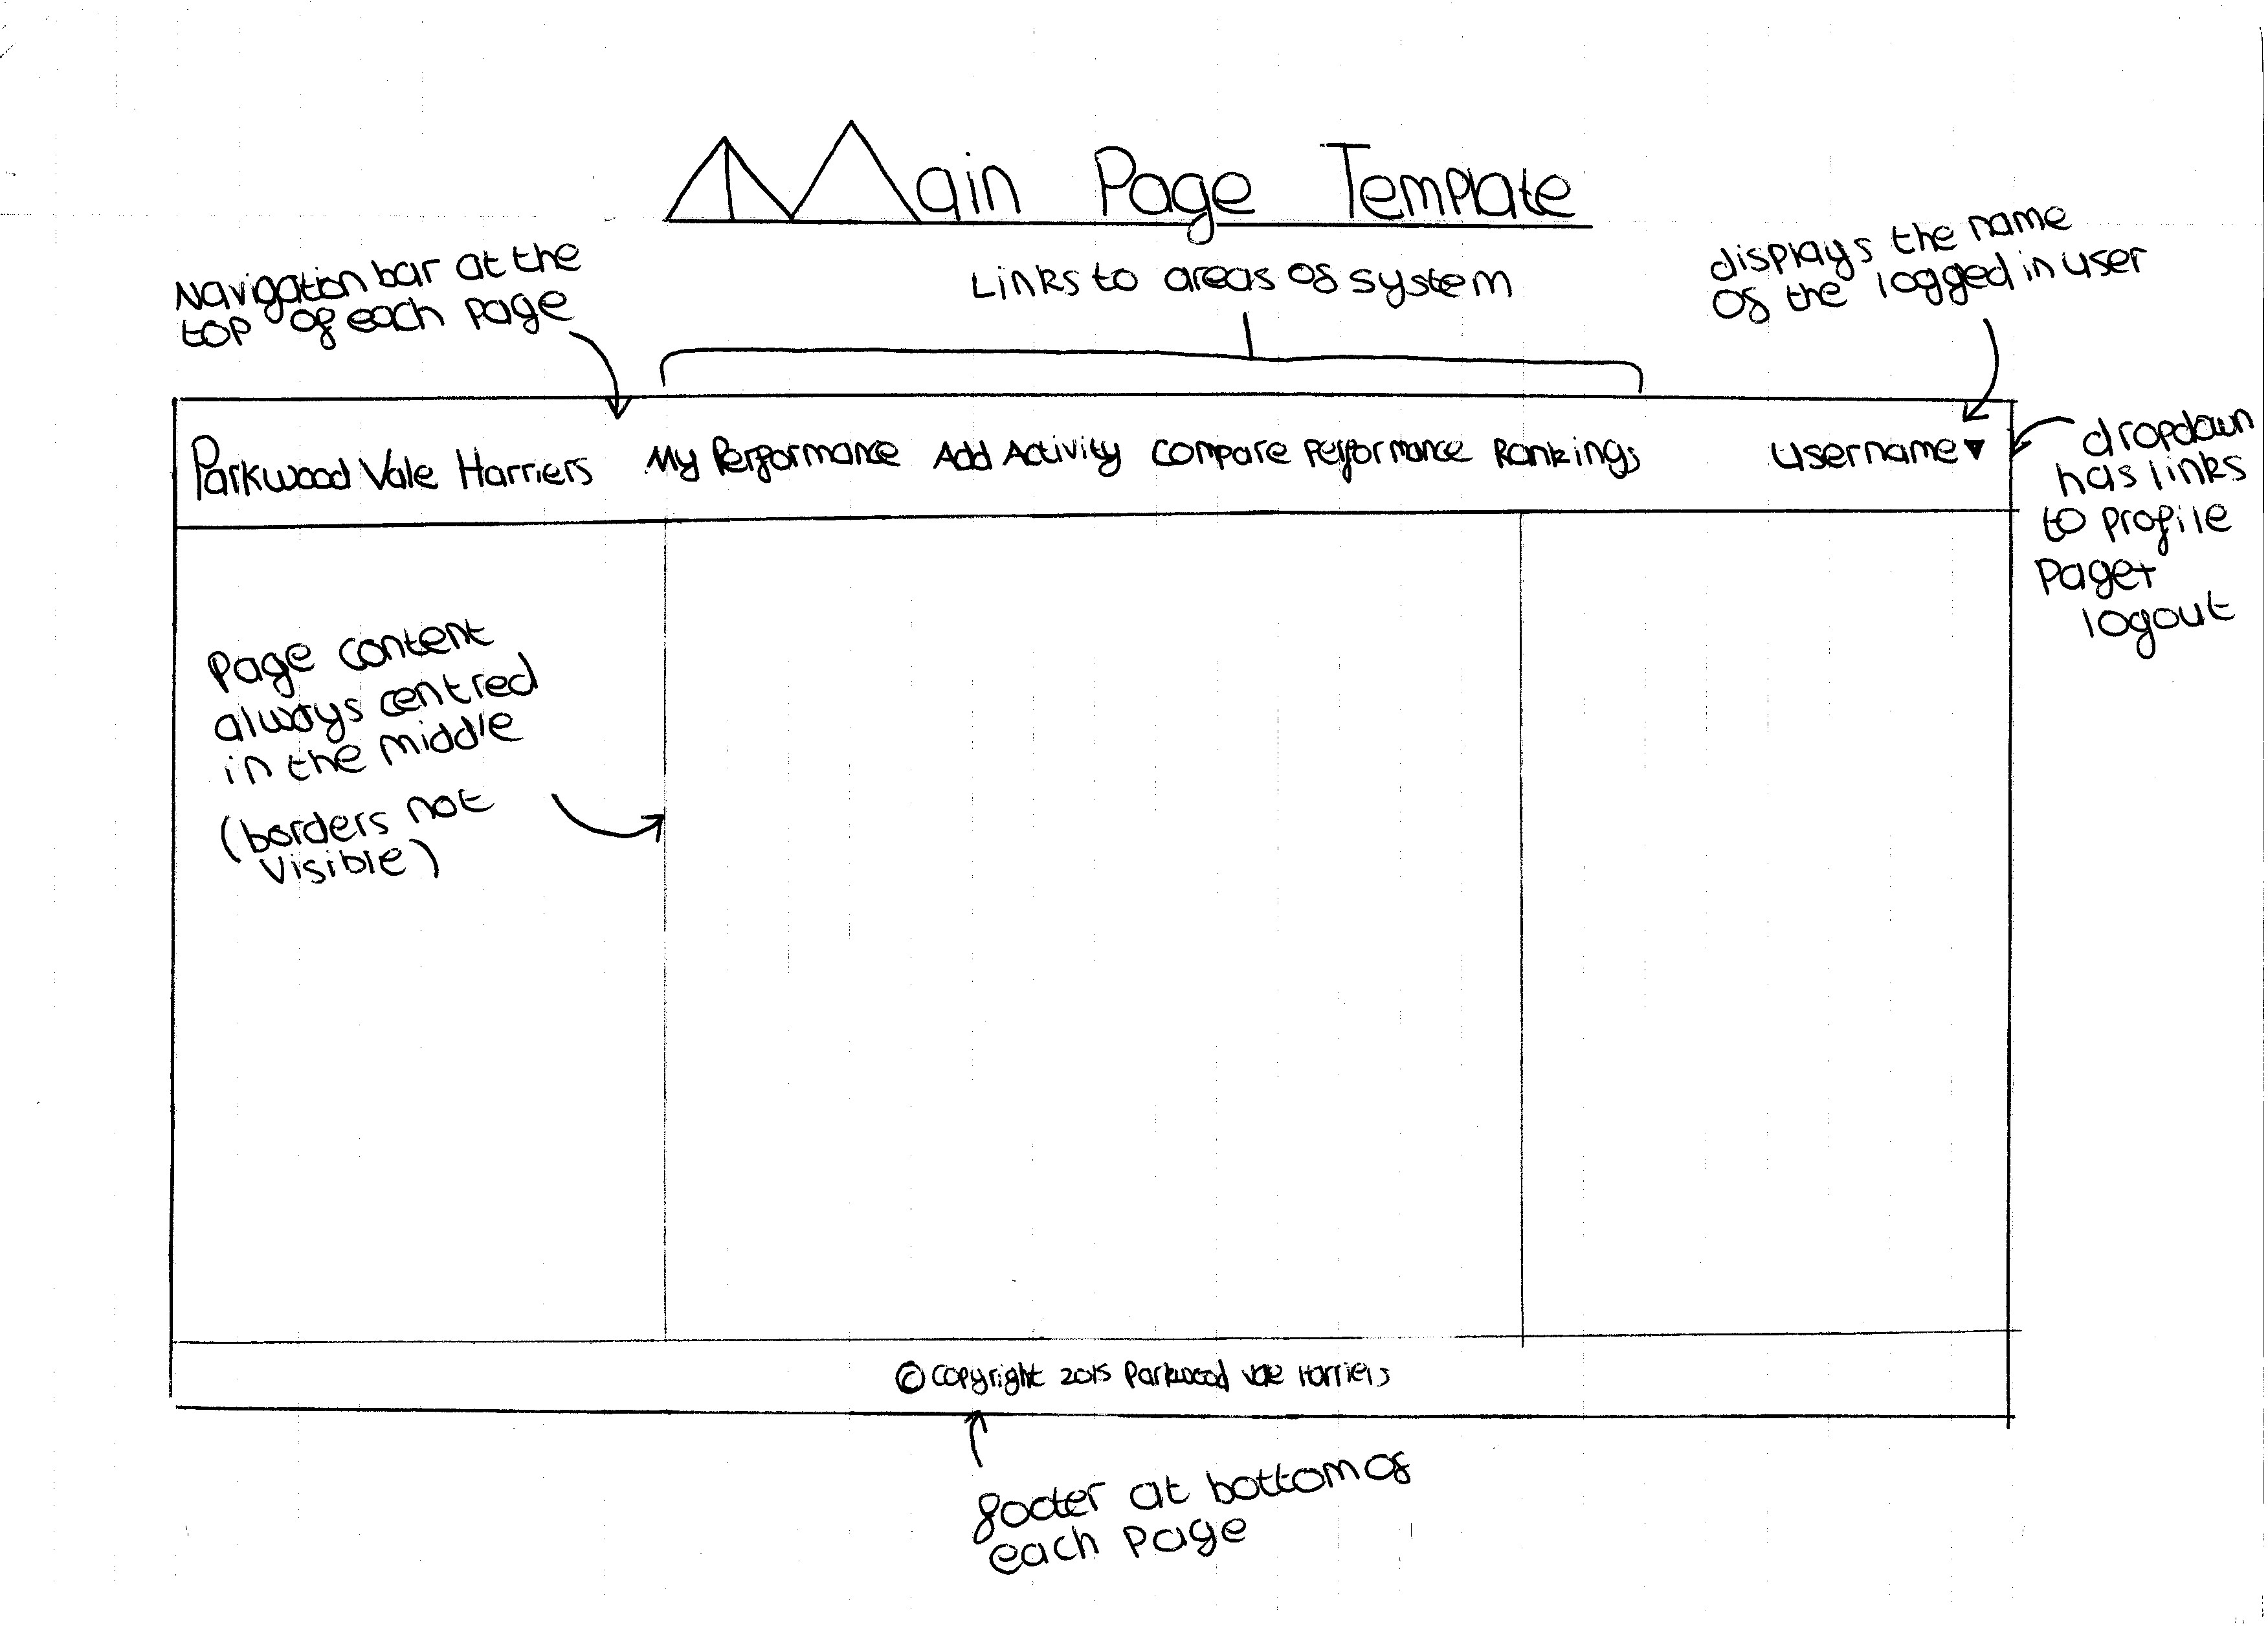
\includegraphics[scale=0.38]{design_ui/layout}
\end{figure}
\clearpage

\subsection{Register Page}
\begin{figure}[h!]
  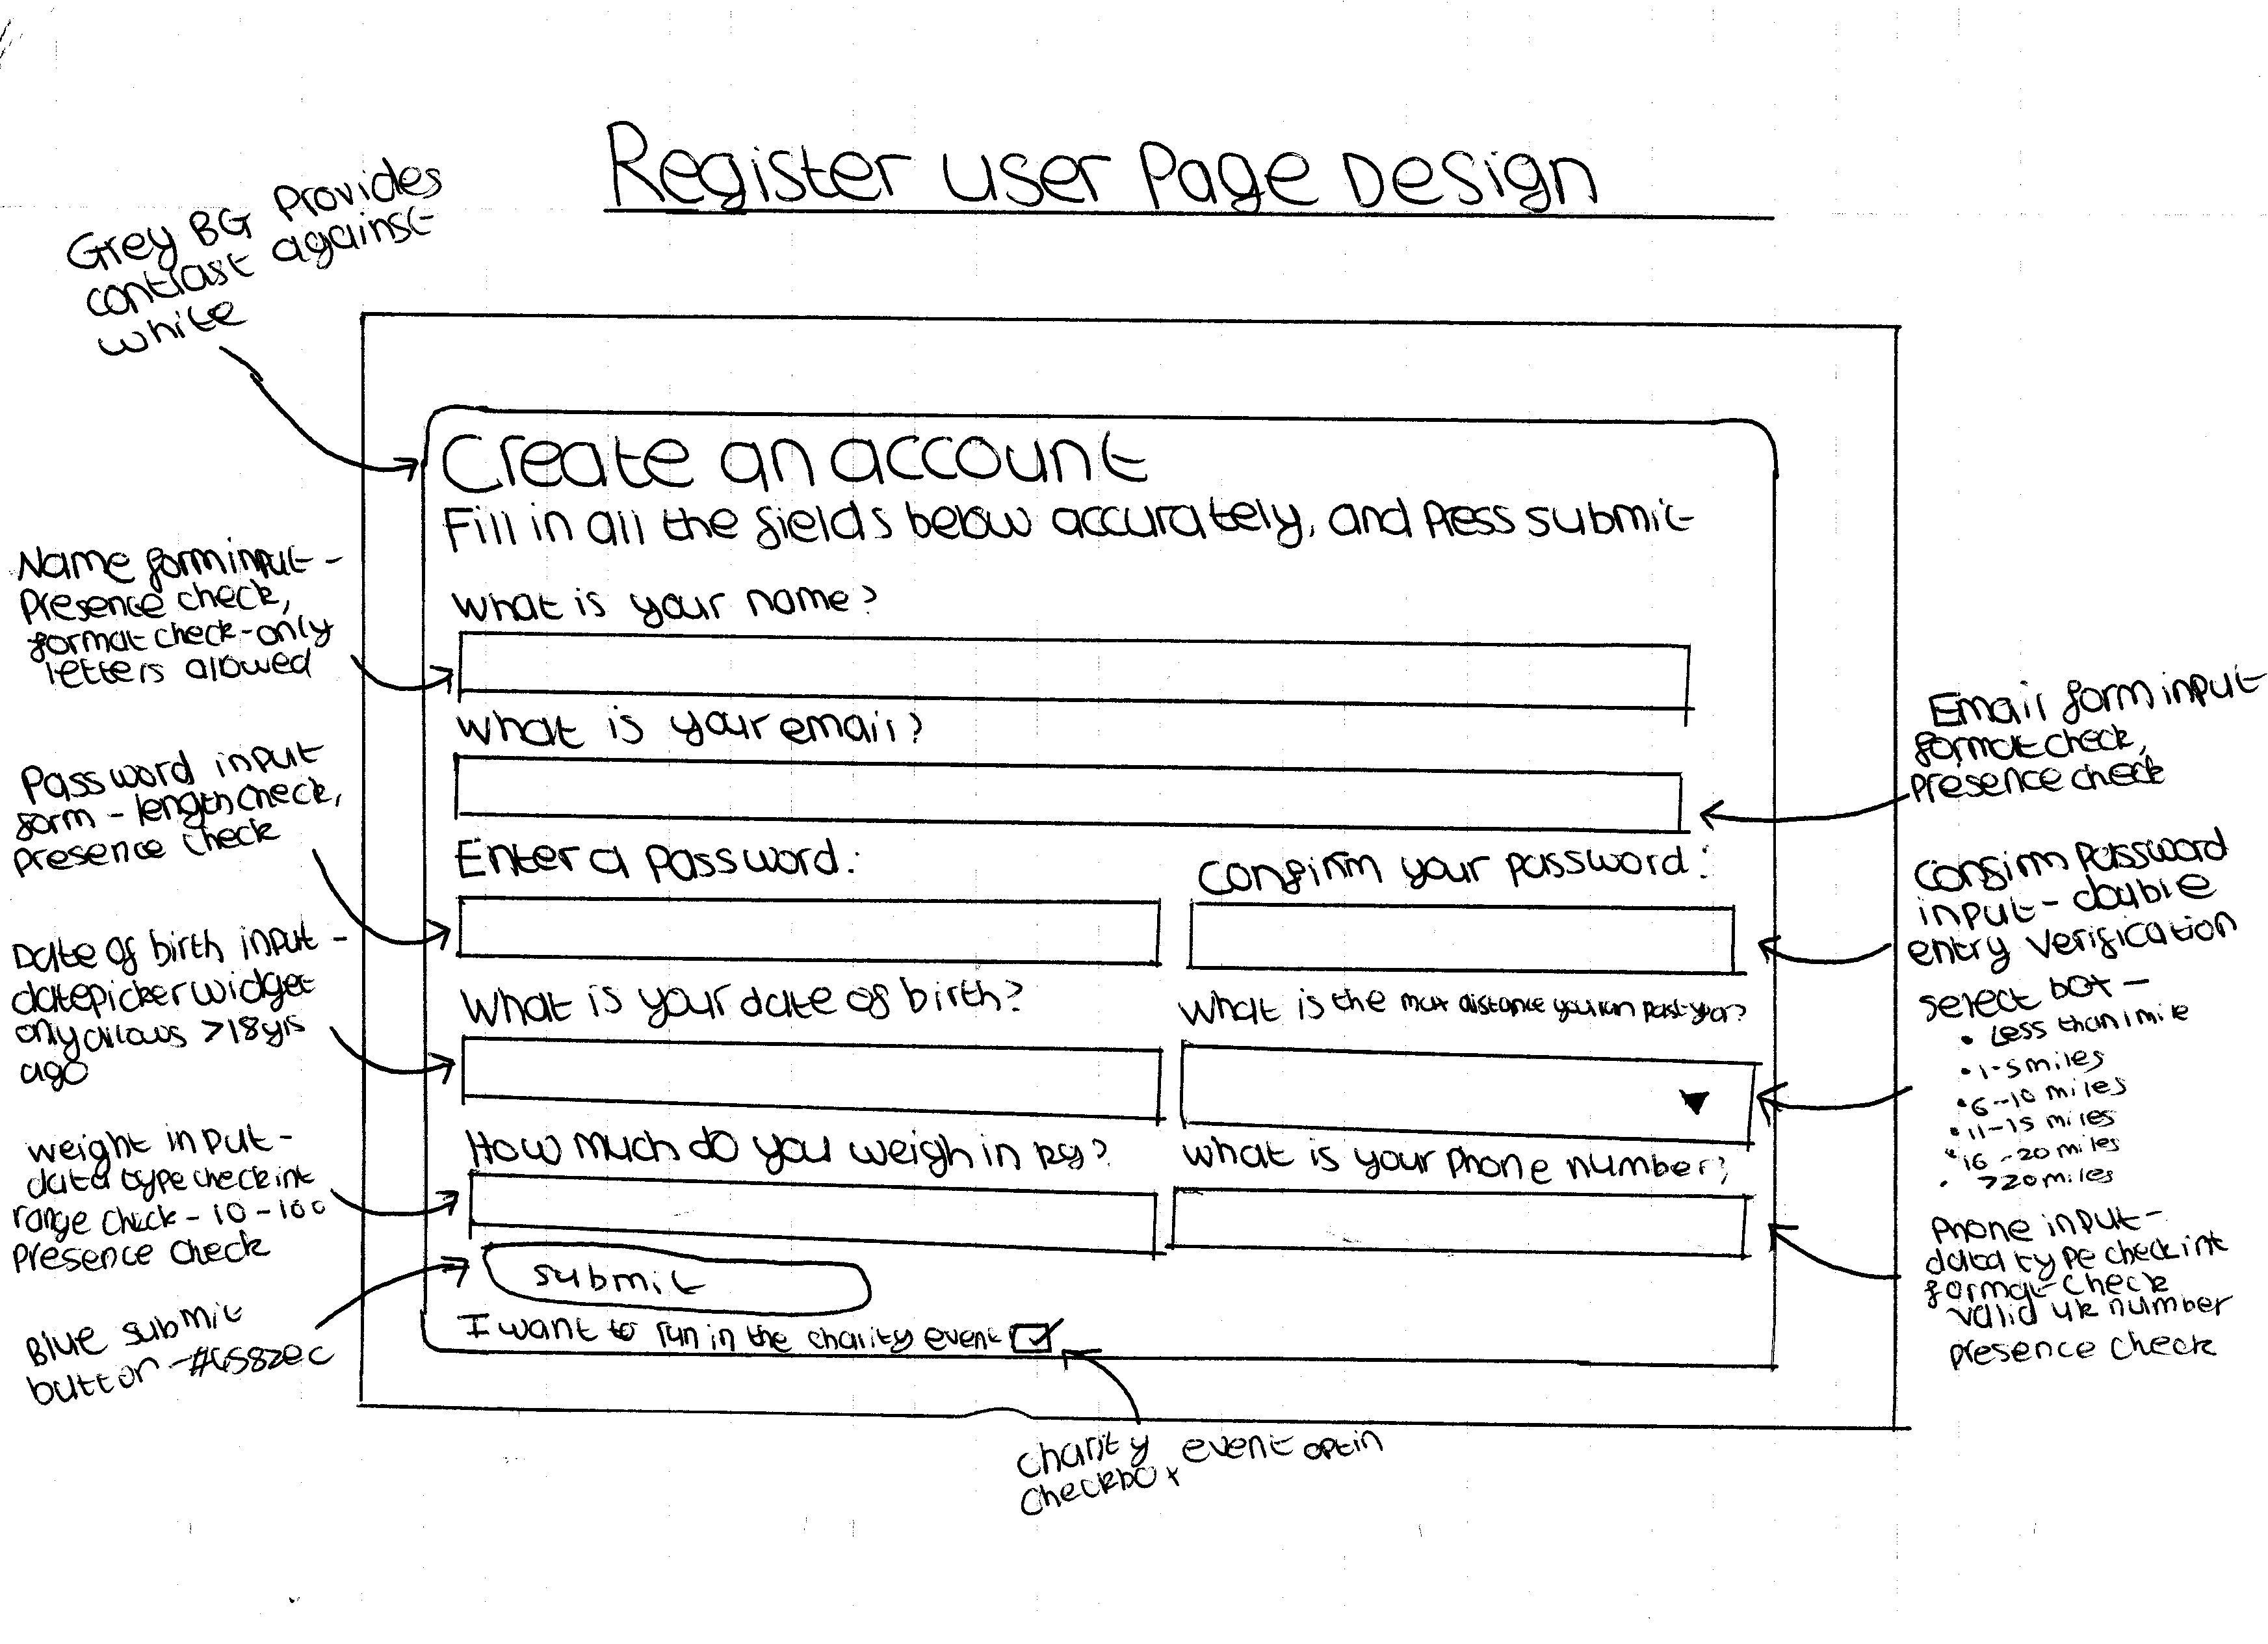
\includegraphics[scale=0.55]{design_ui/register}
\end{figure}
\clearpage

\subsection{Login Page}
\begin{figure}[h!]
  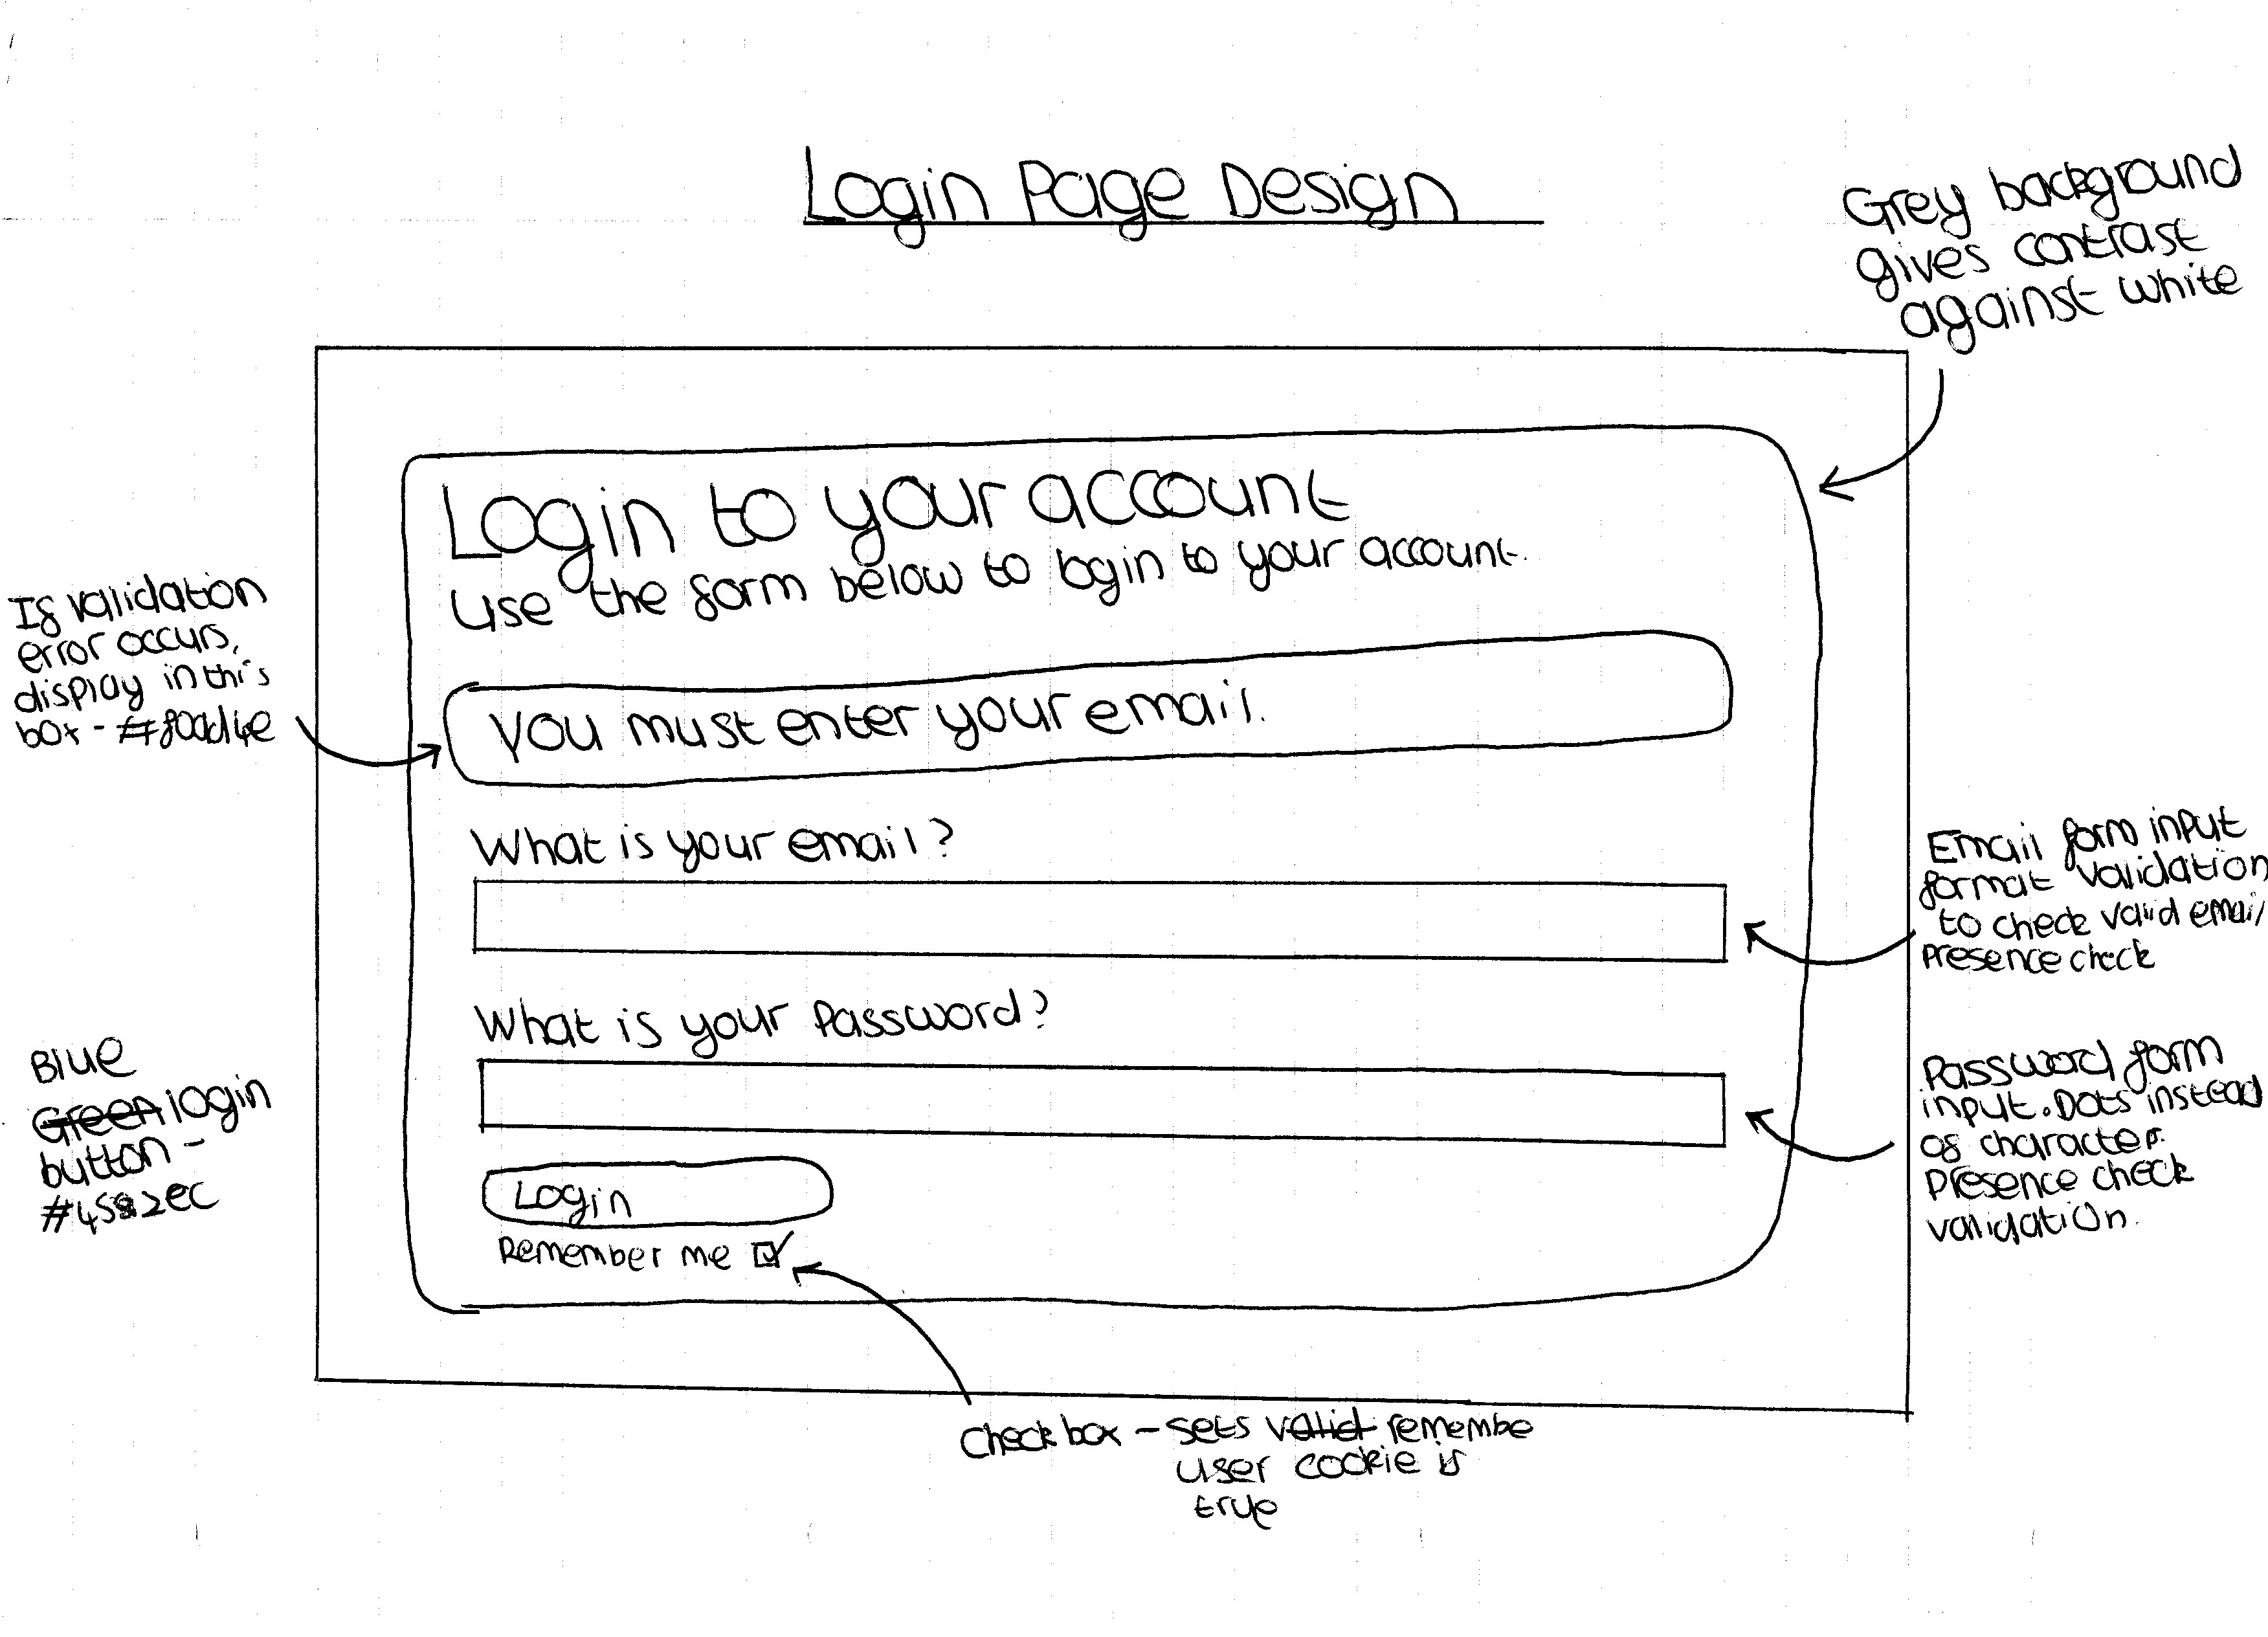
\includegraphics[scale=0.55]{design_ui/login}
\end{figure}
\clearpage

\subsection{Compare Performance Page}
\begin{figure}[h!]
  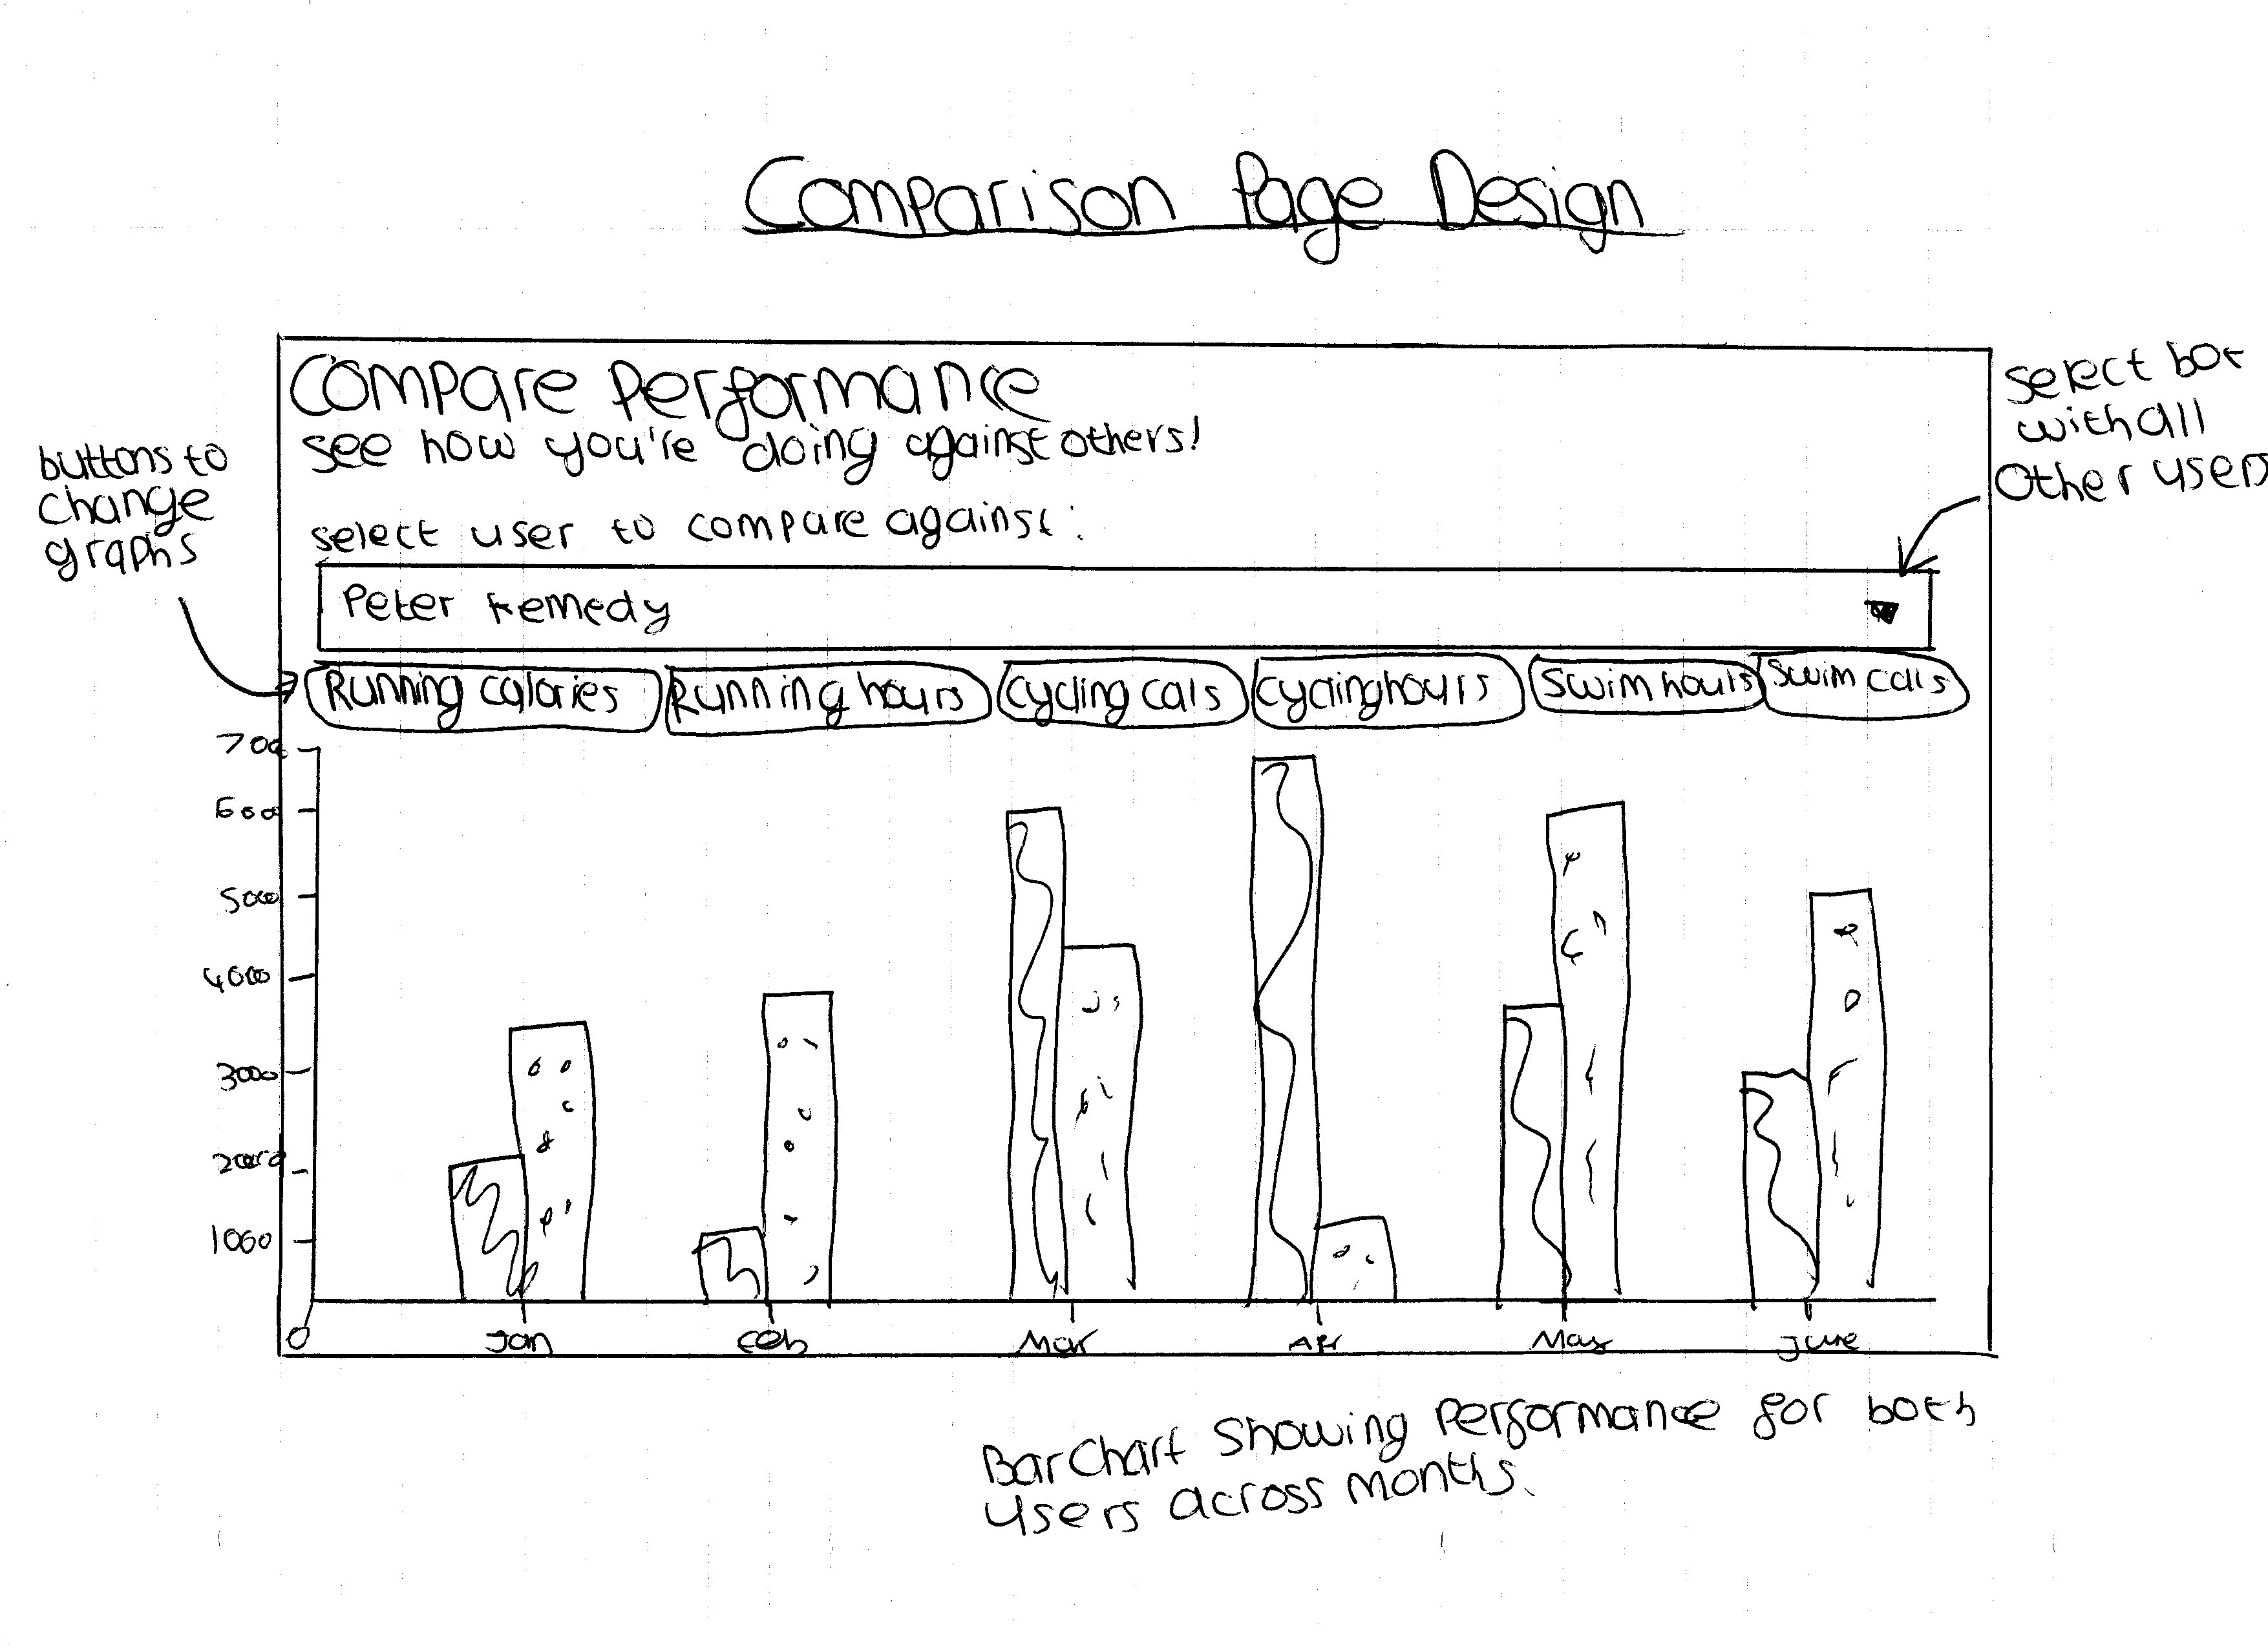
\includegraphics[scale=0.55]{design_ui/compare_performance}
\end{figure}
\clearpage

\subsection{Performance Page}
\begin{figure}[h!]
  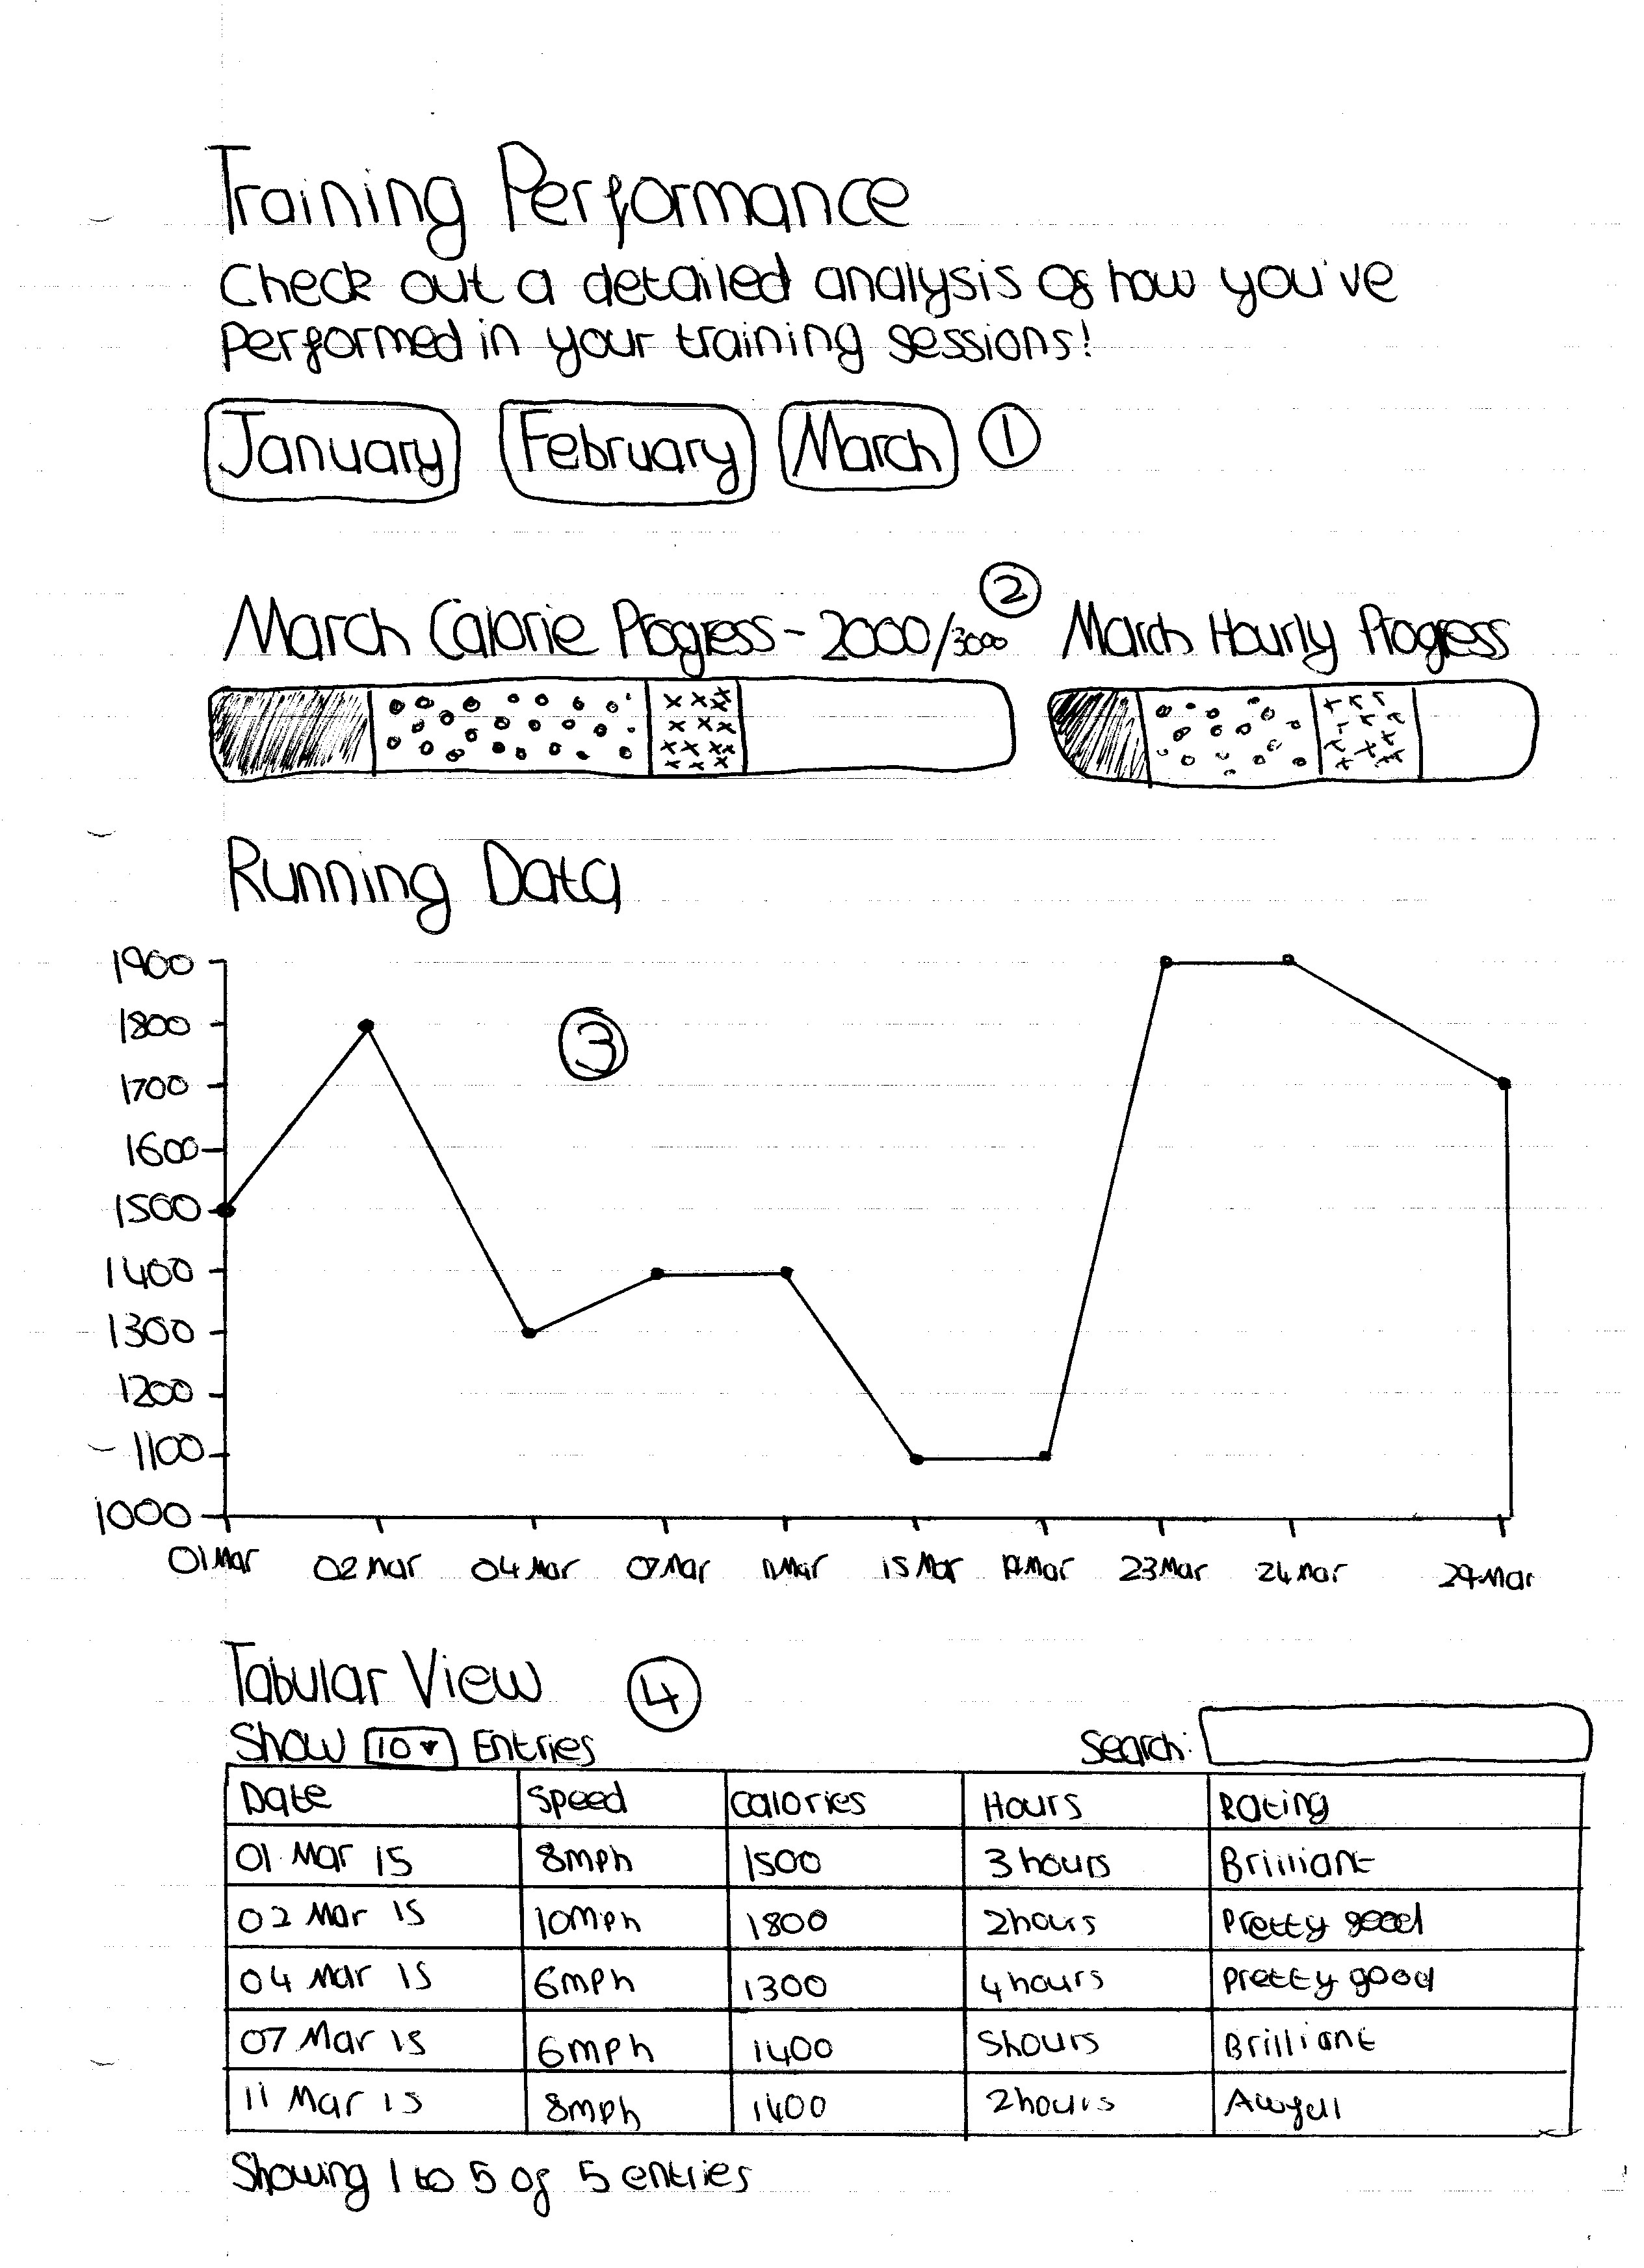
\includegraphics[scale=0.55]{design_ui/user_performance}
\end{figure}
\clearpage

\subsection{Add Training Page}
\begin{figure}[h!]
  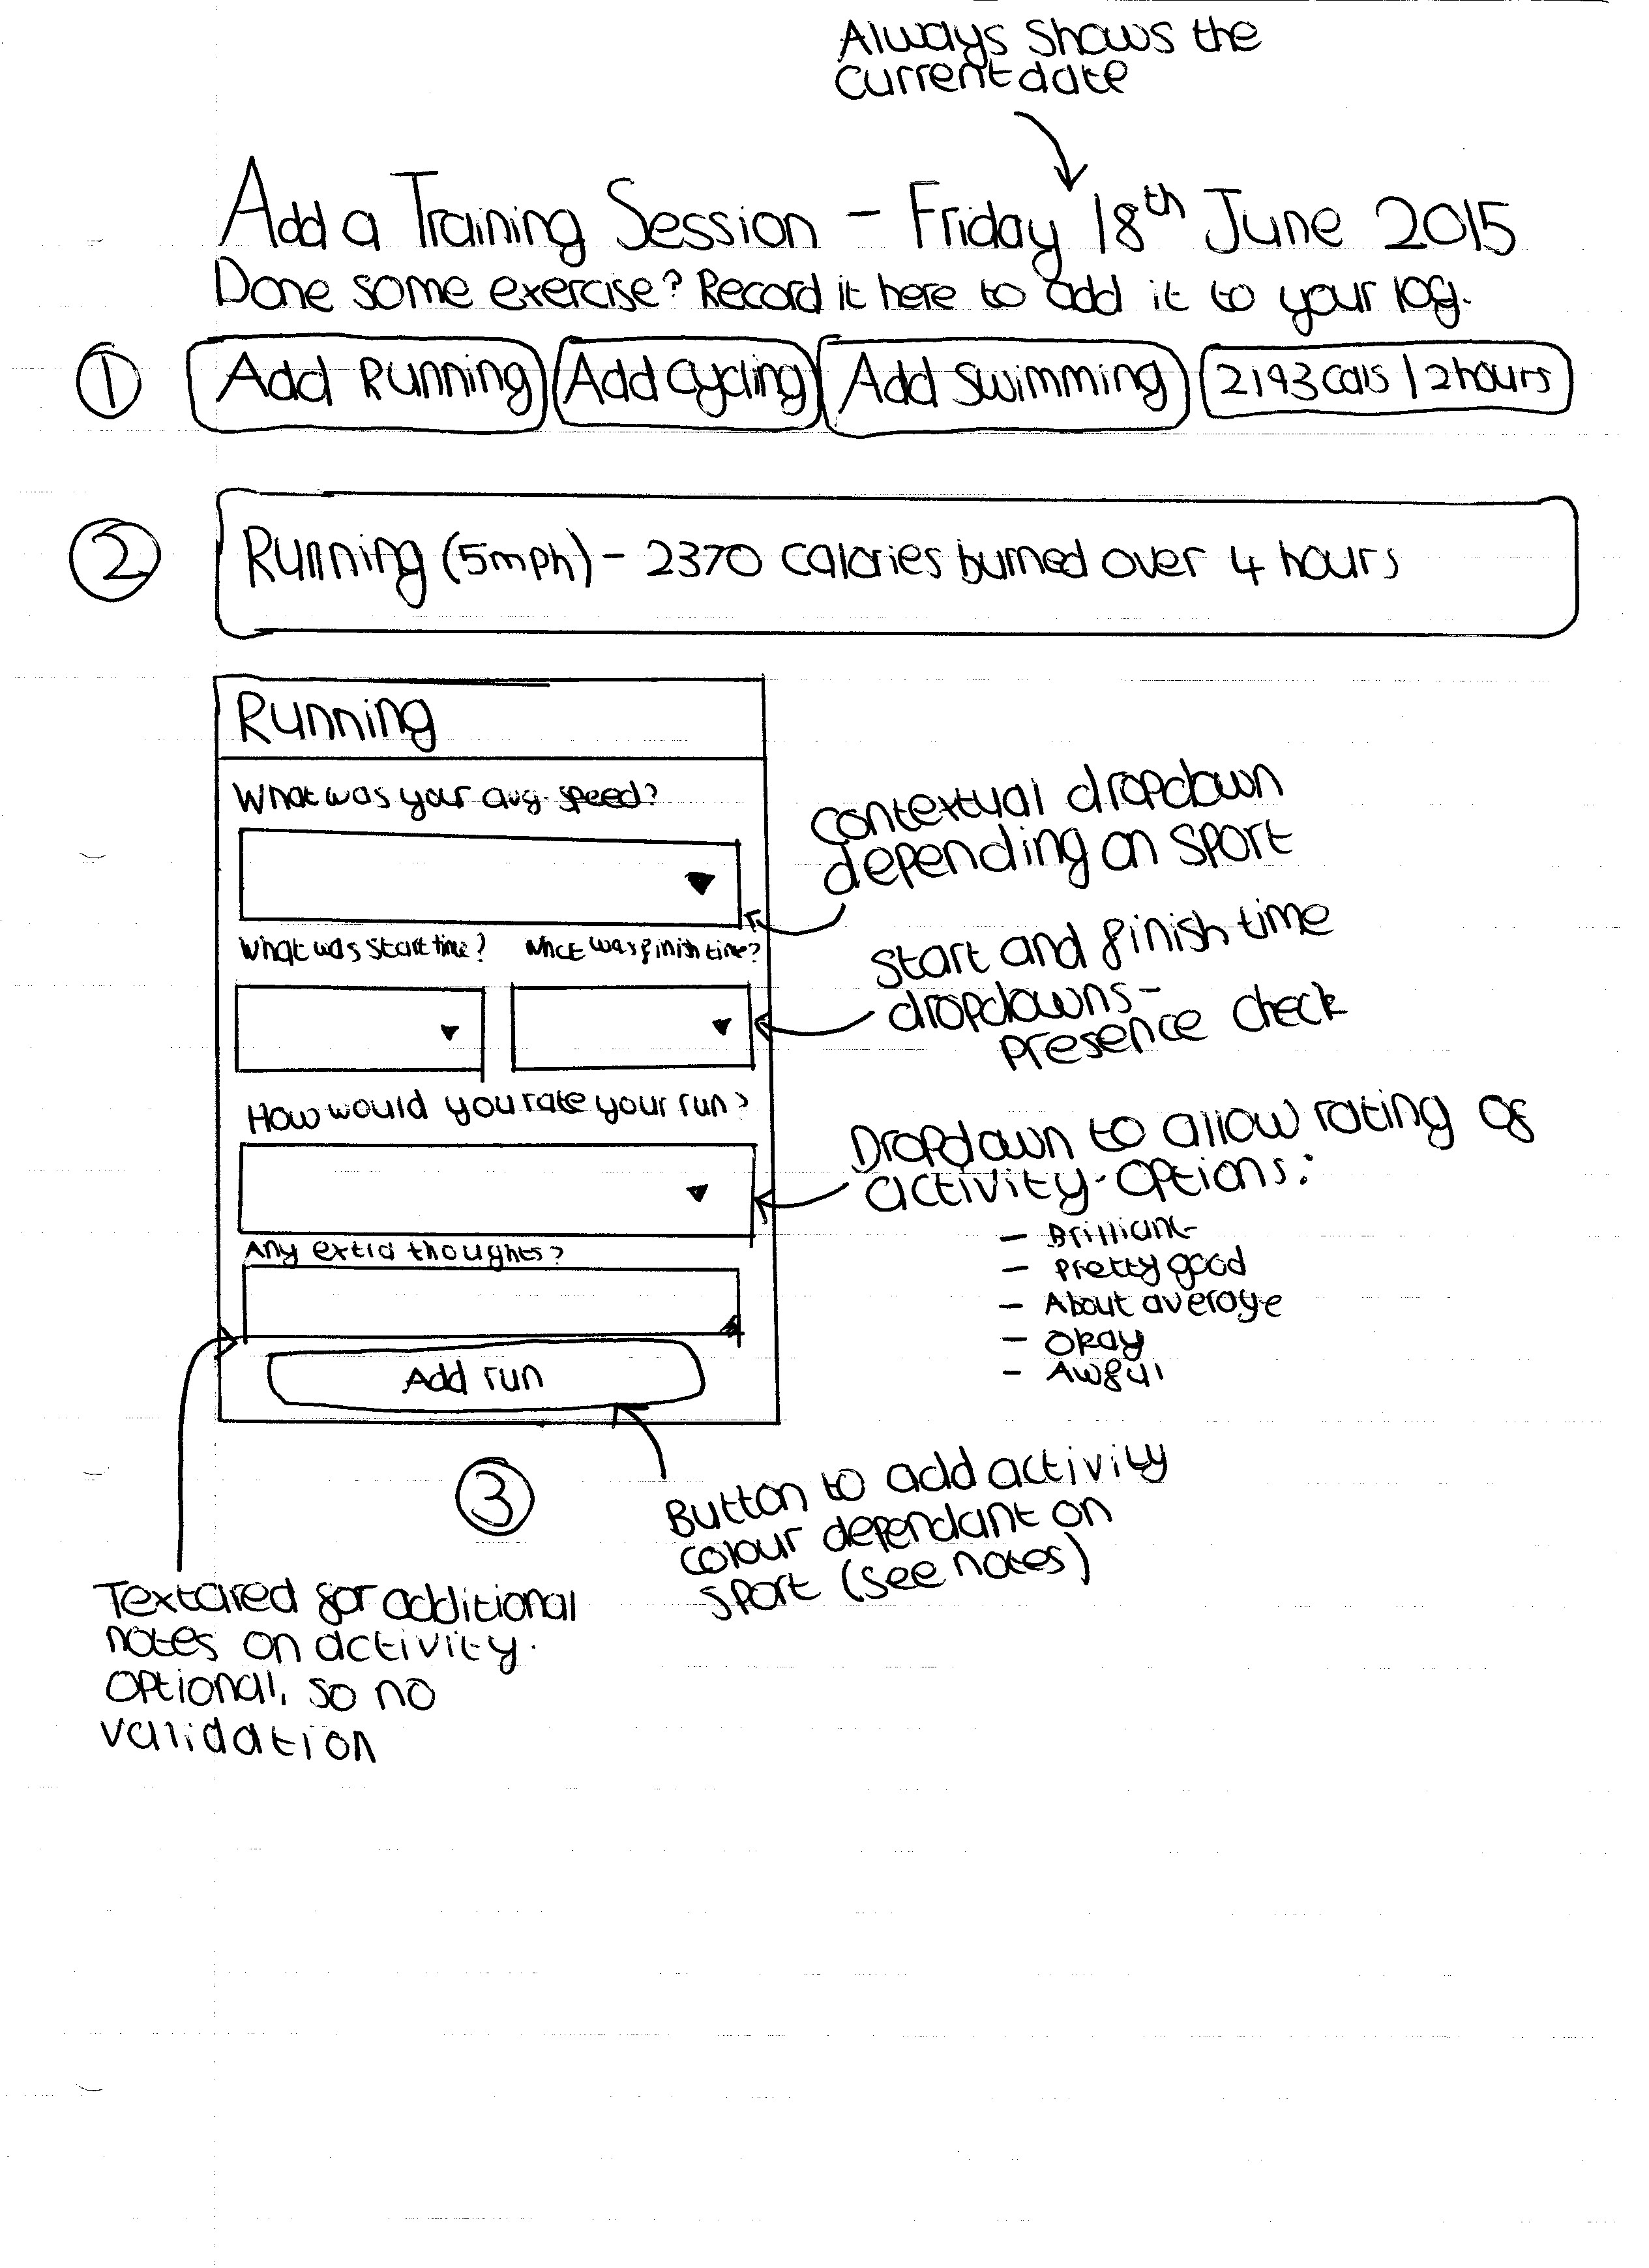
\includegraphics[scale=0.55]{design_ui/add_training}
\end{figure}
\clearpage

\subsection{Profile Page}
\begin{figure}[h!]
  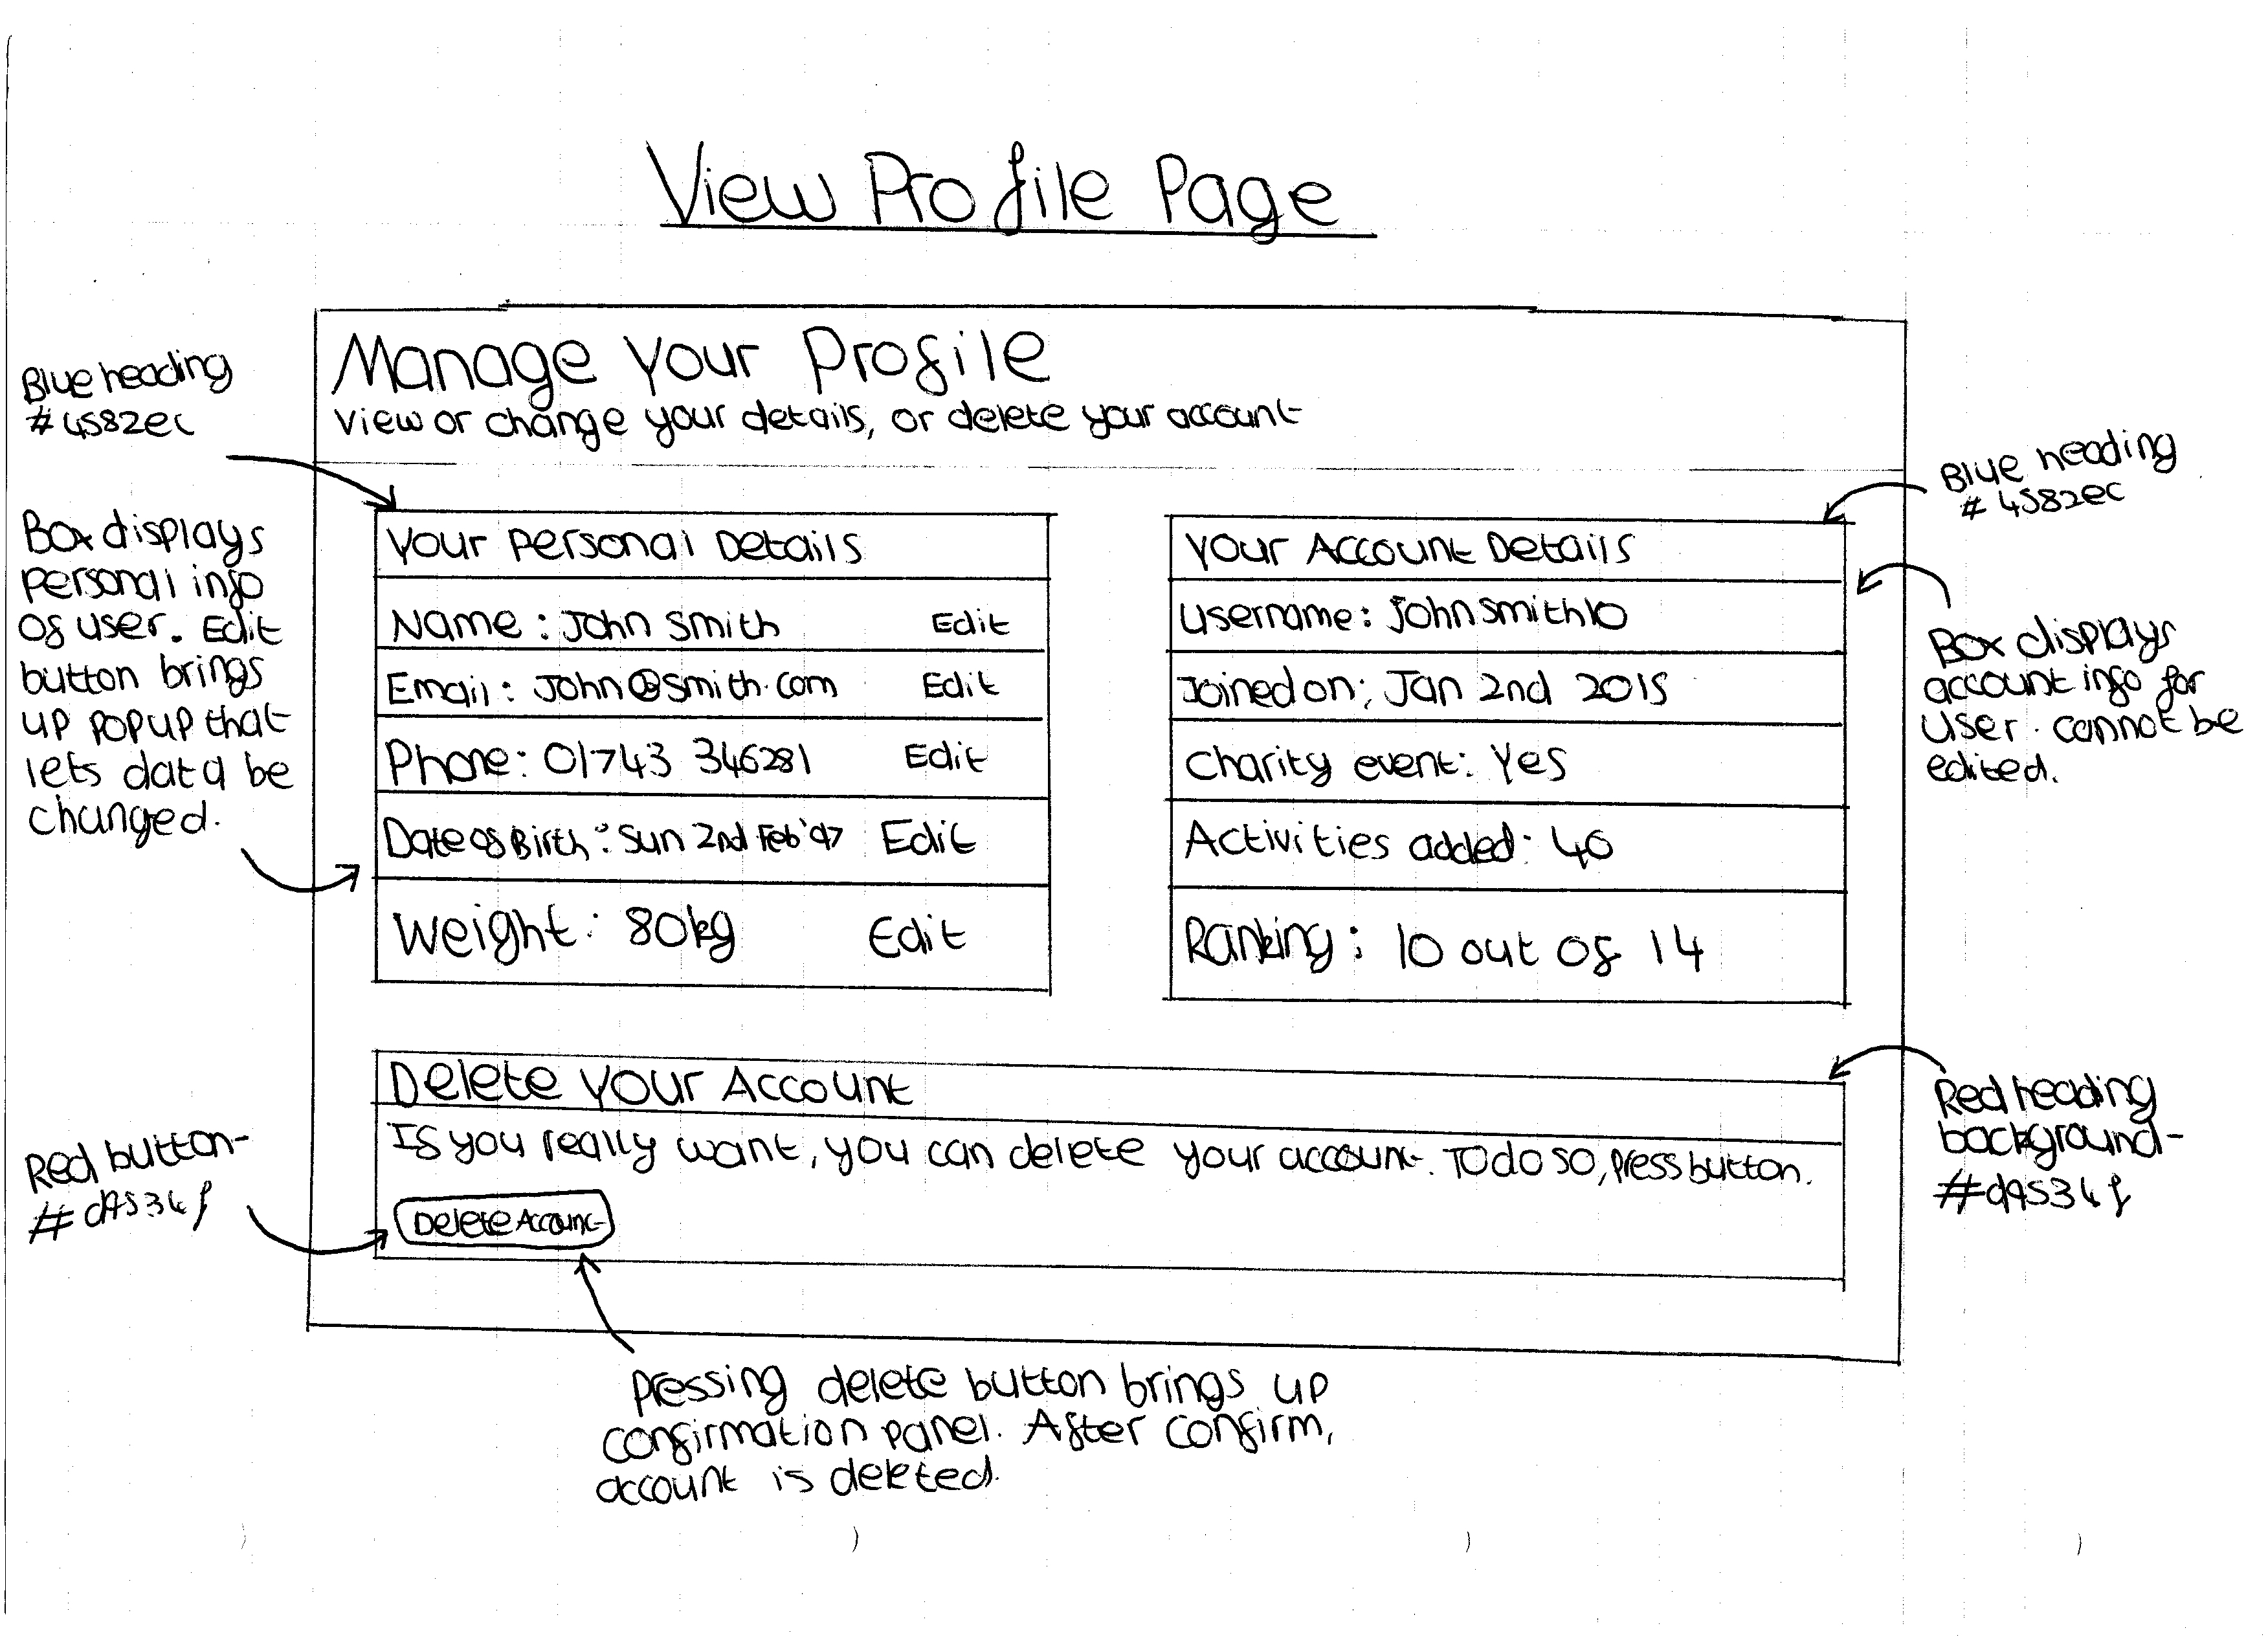
\includegraphics[scale=0.55]{design_ui/profile}
\end{figure}
\clearpage

\subsection{Charity Team Ranking Page}
\begin{figure}[h!]
  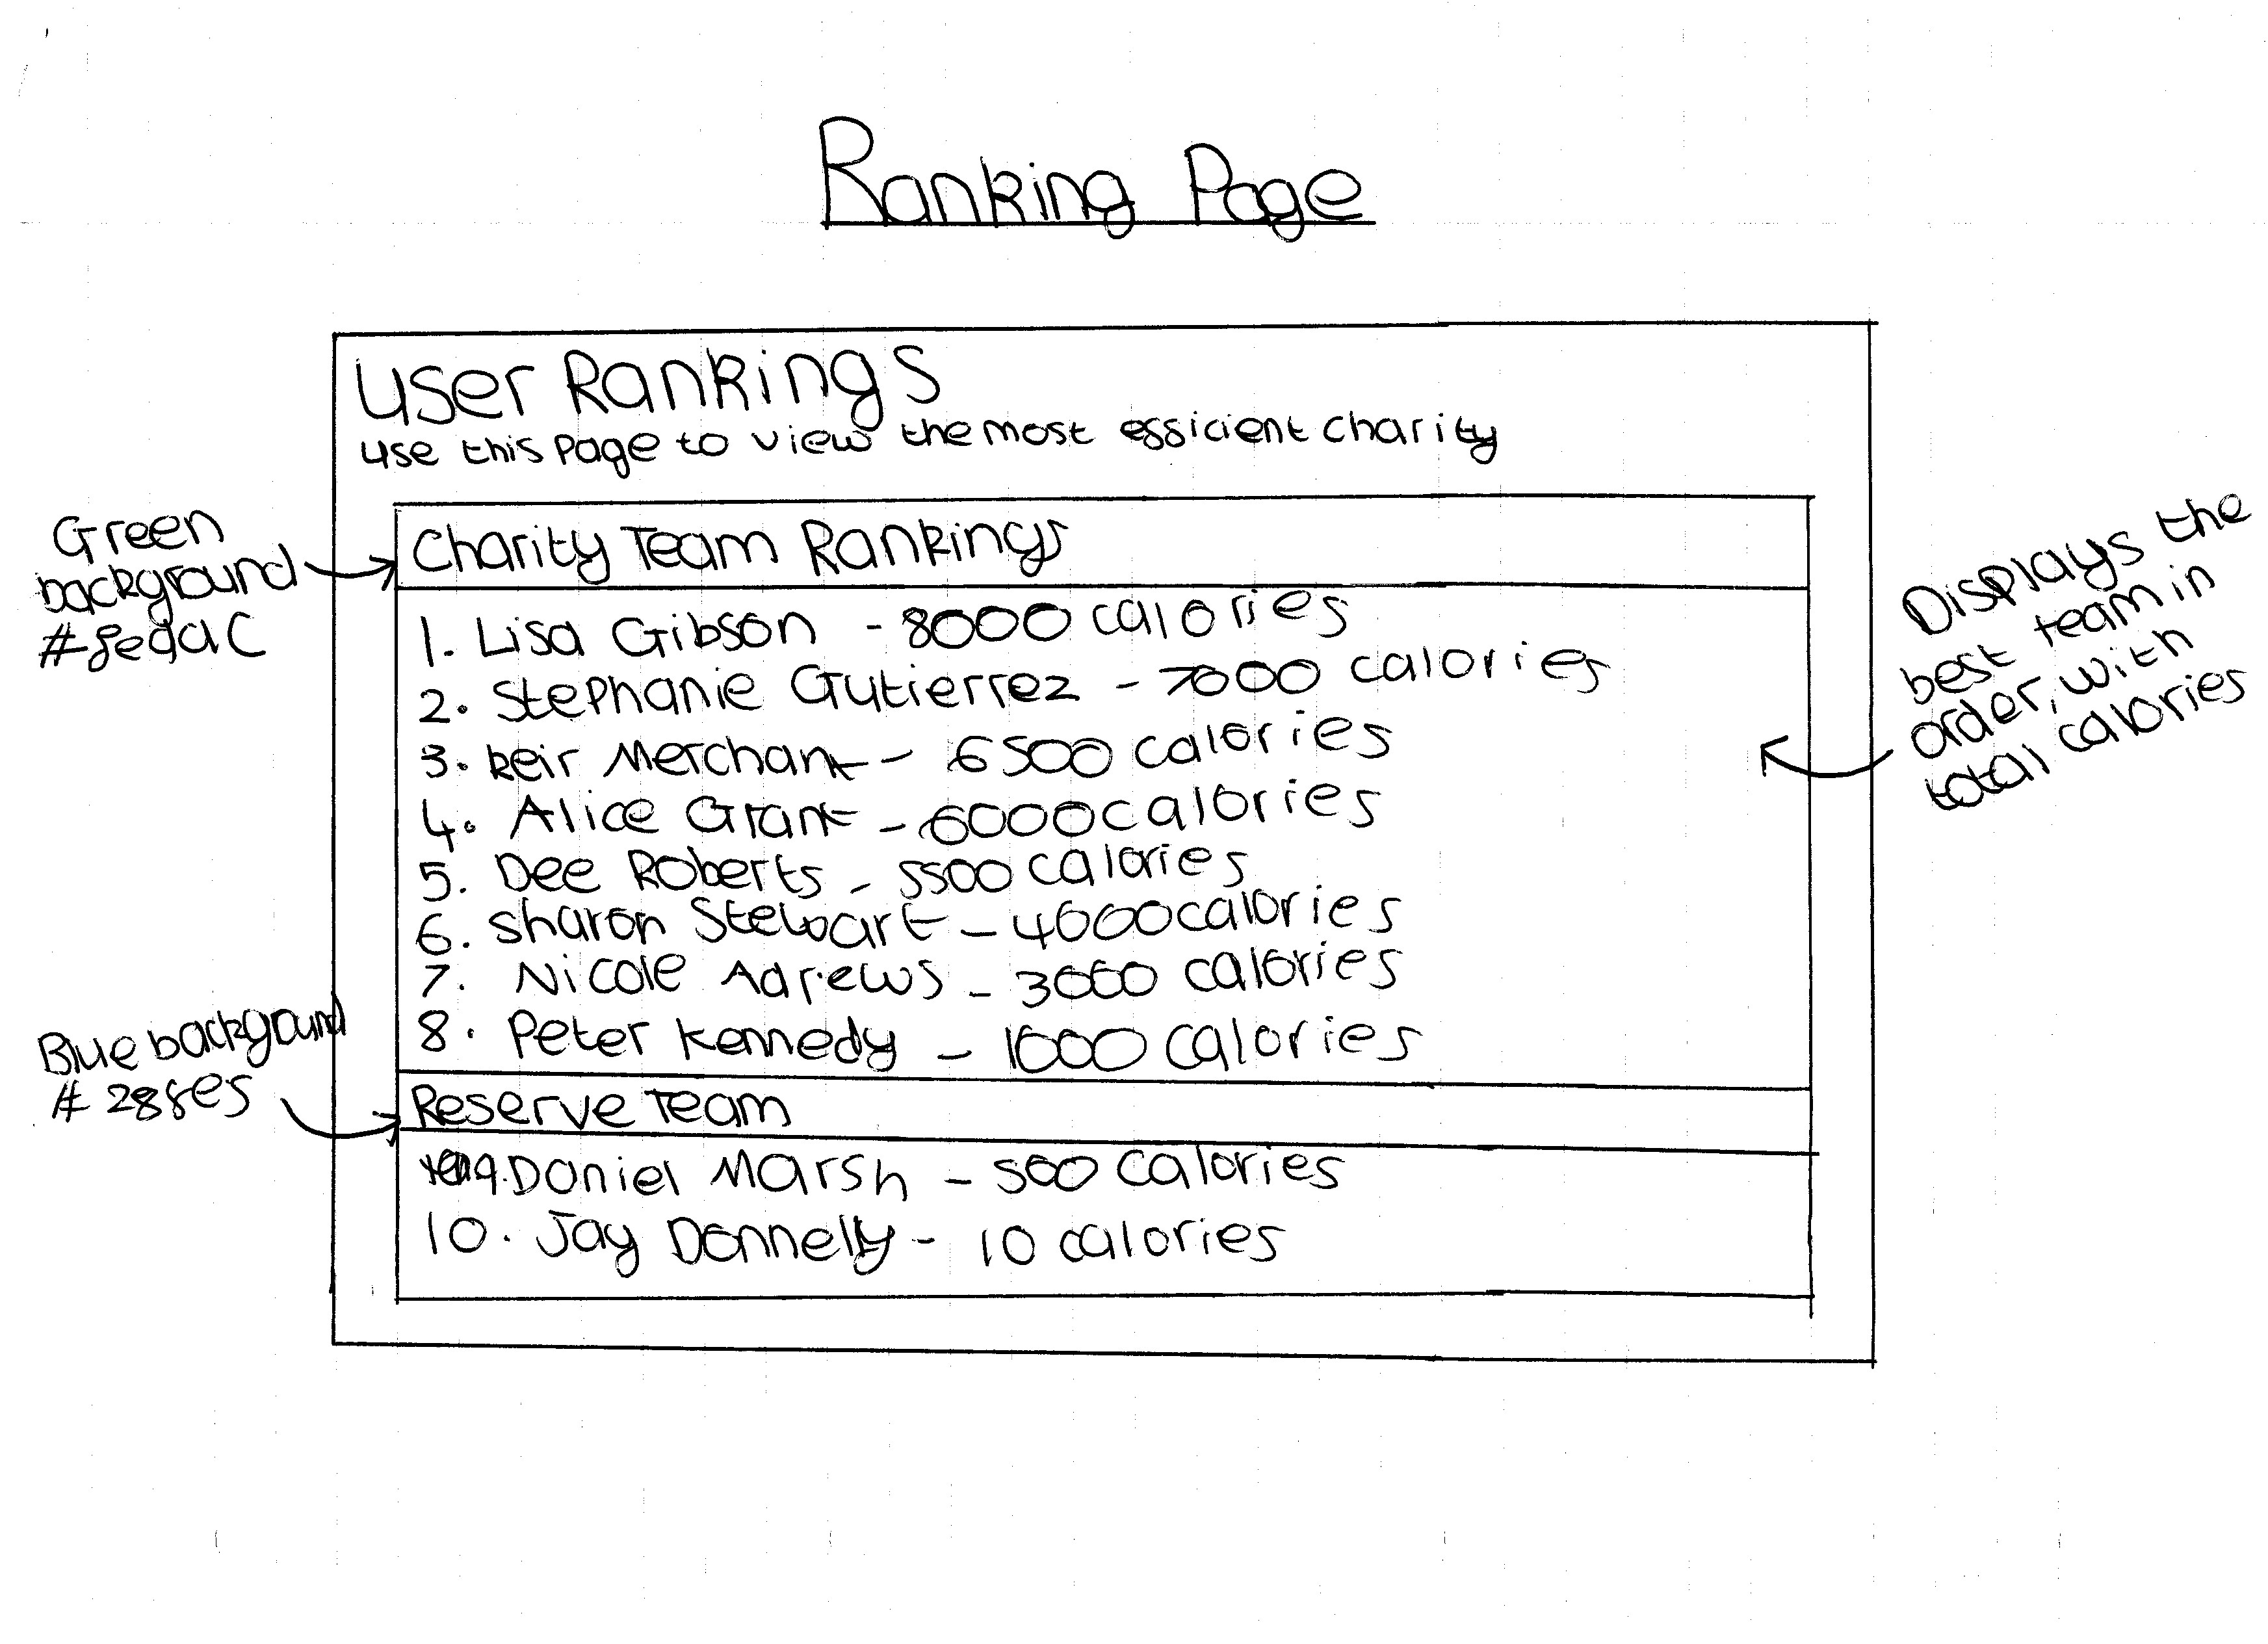
\includegraphics[scale=0.55]{design_ui/rankings}
\end{figure}
\clearpage

\subsection{Page Relationships}
The following hierarchy diagram demonstrates how the different pages of the system will link together.

\begin{figure}[h!]
  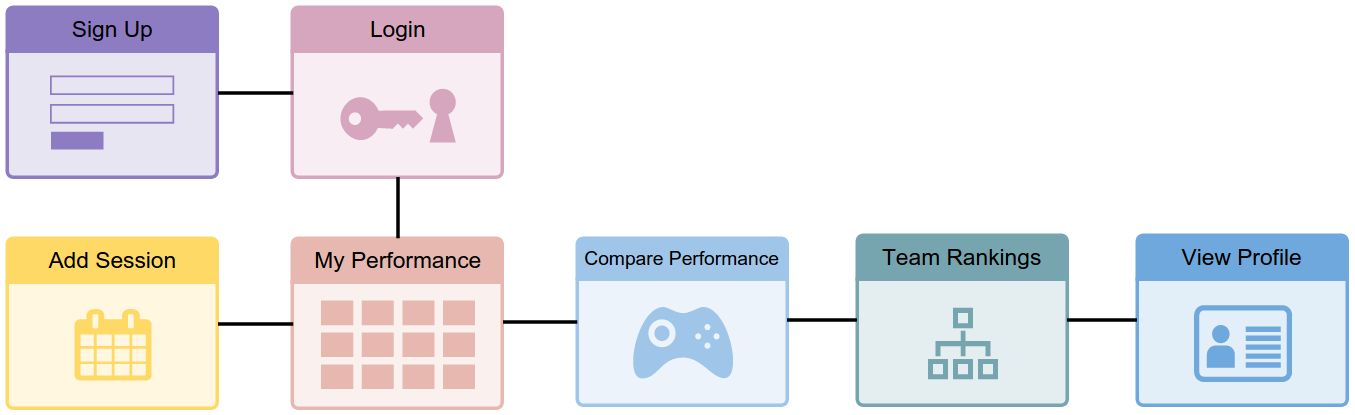
\includegraphics[scale=0.265]{sitemap}
\end{figure}

\noindent
Upon logging in, users will be directed the main performance page, which will show them a range of information about their progress, including graphs for each sport and a table of all their running sessions. For obvious reasons, the signup page links only to the login page, as every part of the application will depend on the user having made an account.


\section{Hardware and Software Requirements}
In order for the system to function correctly, a minimum level of hardware, and some certain software, is needed. A discussion of recommendations in each area can be found below.

\subsection{Hardware}
The system is a web application, and as such requires a stable internet connection to function correctly; therefore, the device used to access the system will need support for the internet, either through a wireless card or an ethernet connection. As a web application, the system can be used on both traditional computing devices, such as desktop PCs and laptops, as well as smart phones and tablets. If using a non touch device, the system has been designed for screens at least 17" in size - a resolution of 1280x1024. The system will function at smaller displays than this, but has not been fully tested as such. Desktops will also requires a mouse, in order to point at and click elements on the page; any mouse is suitable for this task. Additionally, a keyboard is needed for data entry. Laptops usually come with trackpads and keyboards built in, so the need for these additional peripherals is reduced.

If the runner is using a smart phone or tablet - a scenario that is likely, as the audience is a group not known for sitting down at a desk all day - no additional hardware is needed, as the device would come with everything built in, such as a touch screen for interacting with element and a virtual keyboard for data entry. The same internet connection requirements apply.

The hardware need to run the system does not need to be particularly powerful - as it is a web application, it is not memory intensive; as such, only 1GB of RAM would be needed. As most people are no longer living in 2006, a time when 1GB was considered standard, the vast majority of the running club's users should be able to run the system easily. Additionally, the computer would not need a powerful processor; the system should run easily on a system with 1GHz, a clock speed that was considered low end in 2010 - five years ago at the time of writing. 

\subsection{Software}
As a web application, a web browser is the only piece of software needed to access the system - the runner need simply visit the correct web address, and they can access the system. The most suitable browser to open the system in is Google Chrome; luckily, this also happens to be the most popular browser worldwide, so it is likely that they runners are already using it.

 Chrome boasts superior rendering technology to other browsers, as well as greater performance; in addition, all the testing of the system has been performed in Chrome, so it is possible that the system may not function correctly if used in other browsers. 

 Additionally, the runner will need an operating system installed on their computer. Google Chrome is available for Windows, OSX and all Debian/Red Hat distributions of Linux, so their choice of operating system does not matter.

\section{Processing Stages}
This section documents the large range of processes that go into making the system function correctly. It has been split up into a number of sections for organisation. For Python/web development constructs in general that the general reader may find themselves unfamiliar with, an explanation in English has been provided.

\subsection{Global Processes}
A number of processes have been used multiple times throughout the system, such as routing and validation. To avoid writing them out every time they occur, they have been documented here.

\subsubsection{Routing}
The concept of \textit{routing} is fundamental to a Flask application. Practically every function is linked to a route, and every route is linked to a URL. For example, the function auth.login is linked to the URL ``/login'', as makes logical sense. Therefore, visiting the URL ``/login'' will run the code in the function auth.login. 

\begin{verbatim}
@file.route('/url', methods=[METHODS])
begin function route_name:
  begin route logic
  return route result
\end{verbatim}
As can be seen, each route is made up of a number of elements. \textit{file} is equivalent to the file in which the route appears; for example, the function auth.login is in auth.py, therefore its \textit{file} parameter would be set to \textit{auth}. The \textit{url} paramater is equivalent to the URL that the route links to, so for auth.login it would be ``/login'', as written above.

The \textit{methods} parameter specifies which HTTP method(s) can be used to access the route - either \textit{GET}, \textit{POST}, or a combination of the two. A detailed discussion on the differences between the the two is beyond the scope of this explanation, but, put simply, a route with only \textit{GET} specified is designed to be accessed by the runner, whereas those with \textit{POST} are designed for the server (in this system, they are always AJAX routes). A route with both \textit{GET} and \textit{POST} is designed to be accessed by the runner, but it also sends data to the server.

The route logic is the main code for the route. In auth.login, for example, it contains processing to check that their are no validation errors on the form, and for logging the runner in. Every route returns something. For routes with just \textit{GET} or both \textit{GET} and \textit{POST}, this will always be a Jinja2 HTML template, which is then rendered by the browser. For purely \textit{POST} routes, often a JSON object or dictionary is returned, but this varies; see the individual route processes for details.

\subsubsection{AJAX Calls}
AJAX, which stands for \textit{Asynchronous JavaScript and XML}, is a method by which the rendered HTML can interact with the Python server without having to reload the page, creating a smooth experience. The syntax is as follows:

\begin{verbatim}
$.ajax({
  url: `/ajax/ROUTE',
  type: `POST',
  dataType: `DATA_TYPE',
  contentType: `CONTENT_TYPE'
  data: `DATA',
  success: function (data) {
    CALLBACK(data);
  }
});
\end{verbatim}
The \textit{route} parameter defines which route the request should be sent to, as mentioned above. The 
type parameter defines the request type; this is almost always POST, but can be GET on one or two occasions; see specific processes for details. The \textit{data\_type} parameter is set to the type of data that will be sent via the request; this is likely to be JSON in most cases. The \textit{content\_type} parameter is equal to either \textit{application/json} or \textit{text/plain}, depending on the data being sent. The \textit{data} parameter is set to whatever data needs to be sent to the server; this is usually a JSON object or plain text. The \textit{success} parameter is equal to a function that should be run using the data.

\subsubsection{Add Record to Database}
This process will be used multiple times throughout the system in order to make changes to the database. The process for adding to and updating a database in Python is the same, so the same process is used (this process may look sparse, but it really is this simple in Python; only a single line is needed to add to the database - rows and such are created automatically).
\begin{verbatim}
import database from models
add updated object to database session
save database
\end{verbatim}

\subsubsection{Delete Record from Database}
The process for deleting a record from the database in Python is practically identical to adding a record, except a different builtin function is called at the end.
\begin{verbatim}
import database from models
add updated object to database session
delete session
\end{verbatim}

\subsubsection{Query User Table}
Querying the database in Python uses a special syntax that is then converted to raw SQL at runtime. The query parameter is defined when the function is called.
\begin{verbatim}
User.query.filter_by(query).first|all
\end{verbatim}

\subsubsection{Query Activity Table}
Querying the database in Python uses a special syntax that is then converted to raw SQL at runtime. The query parameter is defined when the function is called.
\begin{verbatim}
Activity.query.filter_by(query).first|all
\end{verbatim}


\subsubsection{Presence Validation Check}
Checks whether an input has actually been filled. element is equal to whatever element the process is called on.
\begin{verbatim}
if length of element == 0:
  show message You must enter your \textit{element}
\end{verbatim}

\subsubsection{Format Validation Check}
Checks whether an element matches the correct format, through a regular expression. element is equal to whatever element the process is called on, and regexp is defined at process call.
\begin{verbatim}
if element does not match regexp:
  show message You must enter a valid element
\end{verbatim}

\subsubsection{Length Check}
Checks whether an element is between a certain length. element is equal to whatever element the process is called on, x is equal to the bottom number and y is equal to the top.
\begin{verbatim}
if length of element not between x and y:
  show message You element must be between x and y characters
\end{verbatim}

\subsubsection{Range Check}
Checks whether an element is between a certain length. element is equal to whatever element the process is called on, x is equal to the bottom number and y is equal to the top.
\begin{verbatim}
if element not between x and y:
  show message You element must be between x and y
\end{verbatim}


\subsection{Main Processes}
This section contains all the processes that will make up the application, written in psuedo code. In some cases, a small commentary has been given for explanation.

\subsubsection{Change User Details}
This process is used to modify the personal info of the runner. It checks which element the runner wants to change, and then matches their changed element against a regular expression to ensure they are valid. 

\begin{verbatim}
if request == 'name':
  name_check = [A-Za-z\-" "]
  if name_check matches request:
    set runner to request
    save updated runner to database
  else:
    flash message "invalid name"

elif request == 'email':
  email_check = ^.+@[^.].*\.[a-z]{2,10}$
  if email_check matches request:
    set runner to request
    save updated runner to database
  else:
    flash message ``invalid email''

elif request == 'phone':
  phone_check = \s*\(?(020[78]\)? ?[1-9][0-9]{2} ?[0-9]{4})|(0[1-8][0-9]{3}\)? ?[1-9][0-9]{2} ?[0-9]{3})\s*$
  if phone_check matches request:
    set runner to request
    save updated runner to database
  else:
    flash message ``invalid email''

elif request == 'dob':
  dob_check = dob_regex
  if dob_check matches request:
    set runner to request
    save updated runner to database
  else:
    flash message ``invalid dob''

elif request == 'weight':
  weight_check = ^-?[0-9]+$
  if weight_check matches request:
    set runner to request
    save updated runner to database
  else:
    flash message ``invalid weight''
\end{verbatim}

\subsubsection{Register Page}
On page load:
\begin{verbatim}
  render template register.html
\end{verbatim}

\noindent
On form submit:
\begin{verbatim}
  presence check on email
  format check on email - regexp ^.+@[^.].*\.[a-z]{2,10}$
  presence check on password
  length check on password - 8 - 20 chars
  presence check on confirm
  double entry on confirm - must match password
  presence check on dob
  set today = today.date()

  if today.year - dob.year - ((today.month, today.day) < (dob.month, dob.day)) < 18:
    show message ``You must be at least 18 to signup''

  presence check on phone
   format check on phone - regexp \s*\(?(020[78]\)? ?[1-9][0-9]{2}\s*$
  presence check on weight
  range check on weight - between 10 and 100
  query User table for first where email == email input

  if distance == less than 1 mile and charity_event == true:
    show message ``You must be physically fit to run in the charity event''

  if no validation errors:
    add runner to database
    redirect runner to login page
  else:
    show message Invalid username or password
\end{verbatim}

\subsubsection{Login Page}
On page load:
\begin{verbatim}
  render template login.html
\end{verbatim}

\noindent
On form submit:
\begin{verbatim}
  presence check on email
  format check on email - regexp ^.+@[^.].*\.[a-z]{2,10}$
  presence check on password
  query User table for first where email == email input
  if runner found:
    check password matches
    login_user()
  else:
    show message ``Invalid username or password''
\end{verbatim}

\subsubsection{Calculate Calories Burned}
This function will calculate the number of calories burned in the training session. It builds on the idea suggested in the brief by taking into account how well a runner thought the session went, and also taking into account the weight of the runner.

\begin{verbatim}
  Set base_calories to dictionary: {
    'swimming': {
        'Backstroke': 5.1625, 
        'Breaststroke': 7.375, 
        'Butterfly': 8.1125, 
        'Freestyle (slow)': 5.1625,
        'Freestyle (fast)': 7.375
    },
    'running': {
        '5 mph': 5.9, 
        '6 mph': 7.375, 
        '7 mph': 8.4875, 
        '8 mph': 9.9625, 
        '9 mph': 11.0625, 
        '10 mph': 11.8
    },
      'cycling': {
        'Leisurely': 2.95, 
        'Gently': 4.425, 
        'Moderately': 5.9, 
        'Vigorously': 6.125, 
        'Very fast': 8.85,
        'Racing': 11.8
    },
        'modifiers': {
          'Brilliant': 10, 
          'Pretty good': 5, 
          'About average': 0, 
          'Okay': -5, 
          'Awful': -10}
  }
  Set sport to request['sport']
  Set effigy to request['effigy']
  Set hours to request['hours']
  Set weight to request['weight']

  Set base_value to base_calories[sport][effigy]
  set calories to (base_value * current_user.weight) * hours
  set modifier to base_calories['modifiers'][rating]

  Add modifier to calories

  return calories
\end{verbatim}

\subsubsection{Add Training Session Page}
This function will perform all the processes needed for adding a training session. It will be quite a complicated function, with interaction between a number of different files; therefore it has been split into several sections.


On page load:
\begin{verbatim}
  query Activity table for all activities where date = today and user_id = current_user.id
  set total_hours to 0
  set total_calories to 0

  for activity.hour in today's activities:
    add activity.hour to total_hours
    add activity.calories to total_calories

  render template login.html with today's sessions
\end{verbatim}

\noindent
On add sport button press:
\begin{verbatim}
  AJAX request to /ajax/sport_block. Data parameter name of sport. Data type text/plain.

  if data == `running':
    return running_block.html
  elif data == `cycling':
    return cycling_block.html
  else:
    return swimming_block.html

  Append returned HTML to page
\end{verbatim}

\noindent
On activity block submit:
\begin{verbatim}
  start time input presence check
  finish time input presence check

  if validation passed:
    animate activity block - height -= 100px; width += 1000px

    AJAX request to /ajax/calculate_calories. Data parameter a JSON object containing session hours and rating

    return calculate_calories()
    save activity to database
\end{verbatim}

\subsubsection{Calculate Running Team}
Calculates the running team. Calculates the total calories burned for each runner who opted into the charity event, and then sorts this by the highest number. Displaying the top 8 is performed in the Jinja template; beyond the scope of this.

\begin{verbatim}
set user_ranking to empty dict
set runners to db query for all runners who opted into charity event

for runner in runners:
  set total_calories = 0
  set training_sessions to db query for all of runner's activities

  for session in training_sessions:
    add session.calories to total_calories
  set user_ranking[runner.name] to total_calories

sort user_ranking using built in Python sorted function
\end{verbatim}

 
\section{Evaluation Criteria}
This section contains a number of criterion that the system will be judged upon to determine the extent to which it has been successful. It has been split into two sections: measurable criteria, which can be easily determined; ie. the system has met this point irrefutably, because the evidence is visible. Non-measurable criteria have also been included; these are somewhat more subjective, but still provide a useful base upon which the system can be based.

\subsection{Measurable Criterion}
The running club has commissioned  a computer based system that will allow runners to keep an accurate record of their running, cycling and swimming sessions. This data will then be used to calculate an informed decision of most appropriate team for relay race.

The system must allow each runner to monitor their progress during programme, clearly showing them extent to which they have improved. As such, the system must provide an interface to allow runner to add each session they perform, with spaces for type of training, time spent, how hard they pushed themselves, and other such parameters. Using this data, the system must then calculate number of calories burned in session, providing a series of data points through which performance of runner can be monitored.

To further aid in this, the system must be able to output these sessions in a clear format that runner is able to clearly understand. This can be achieved through use of tables to display each session in a listed, tabular format, as well as through graphs and charts to display data in a graphical form; this maes overall performance trends easy to visualise.

Due to nature of the system, ability to store certain personal information, such as name, age and weight of runner, must also be included. runner should have ability to input this information themselves, most likely upon first use of the system. There should be ability to modify this data, in result of an error being made or circumstances of runner changing.

An important aspect of the system, and one that is key to promoting competitive values of club, is ability to compare results with other participants in program. This area of the system should allow runners to compare key aspects of their performance, such as results of their individual sessions, as well as their overall performance over time in all three of activities.

As the main point of the system, ability to select final team must also be included. By analysing data points provided by runners, the system should be able to choose most appropriate team.

The system should also have appropriate validation for each input, to ensure that no erroneous data is added into the system; this would result in errors, likely causing the system to crash.

Additionally, the calculations performed by the system should be accurate, to ensure that the runner is not given false data, and that the system does not calculate an incorrect running team.

The system must also be able to add a training session in at least 2 seconds from when the runner clicked the add button, and the database should be able to store at least 100 users.

\subsection{Non-Measurable Criterion}
The system should be very easy to use. It should have sensible, coherent navigation to allow the runner to easily move between each section of the system. 

Additionally, the system should have a consistent layout on each of the pages; this will serve to ensure that the runner does not get lost when navigating through the system: the navigation bar, logo and footer should always be in the same location.

It is also important that the buttons and other controls, such as inputs, on the form are easy for the runner to understand - they should know exactly what each button does, and what the program will do when they click it. 

Furthermore, the system should have a consistent ``house style'': the same colours should be used for similar elements, and the typography used should be the same throughout every page. Headings should always be kept the same size, depending on their importance - one H3 level header should not be 20px whilst another is 25px.

The classes and variable names given to different elements of the code should be appropriate and be self-documenting: for example, the running graph should not be called \textit{g\_ru}, as this is not specific enough, and would make maintenance on the system very difficult.
\cleardoublepage


\part{Program Documentation}
This second part of the documentation contains a number of sections concerning the finished application. It includes aspects like screenshots of the finished system, as well as a brief discussion of how they are fit for purpose; detailed information on the final database tables, including a diagram detailing their links; a list of every variable used throughout the system, both global and local in scope; and annotated, self-documenting code listings for the entire source of the system, detailing exactly how it works.

\section{User Interface}
This section contains screen captures of all different areas of the completed the system, along with additional notes stating how they are fit for purpose.

\subsection{Main Layout}
Every other page derives constant elements, like the navigation bar and footer, from this template, to ensure visual consistency.

\begin{figure}[h!]
  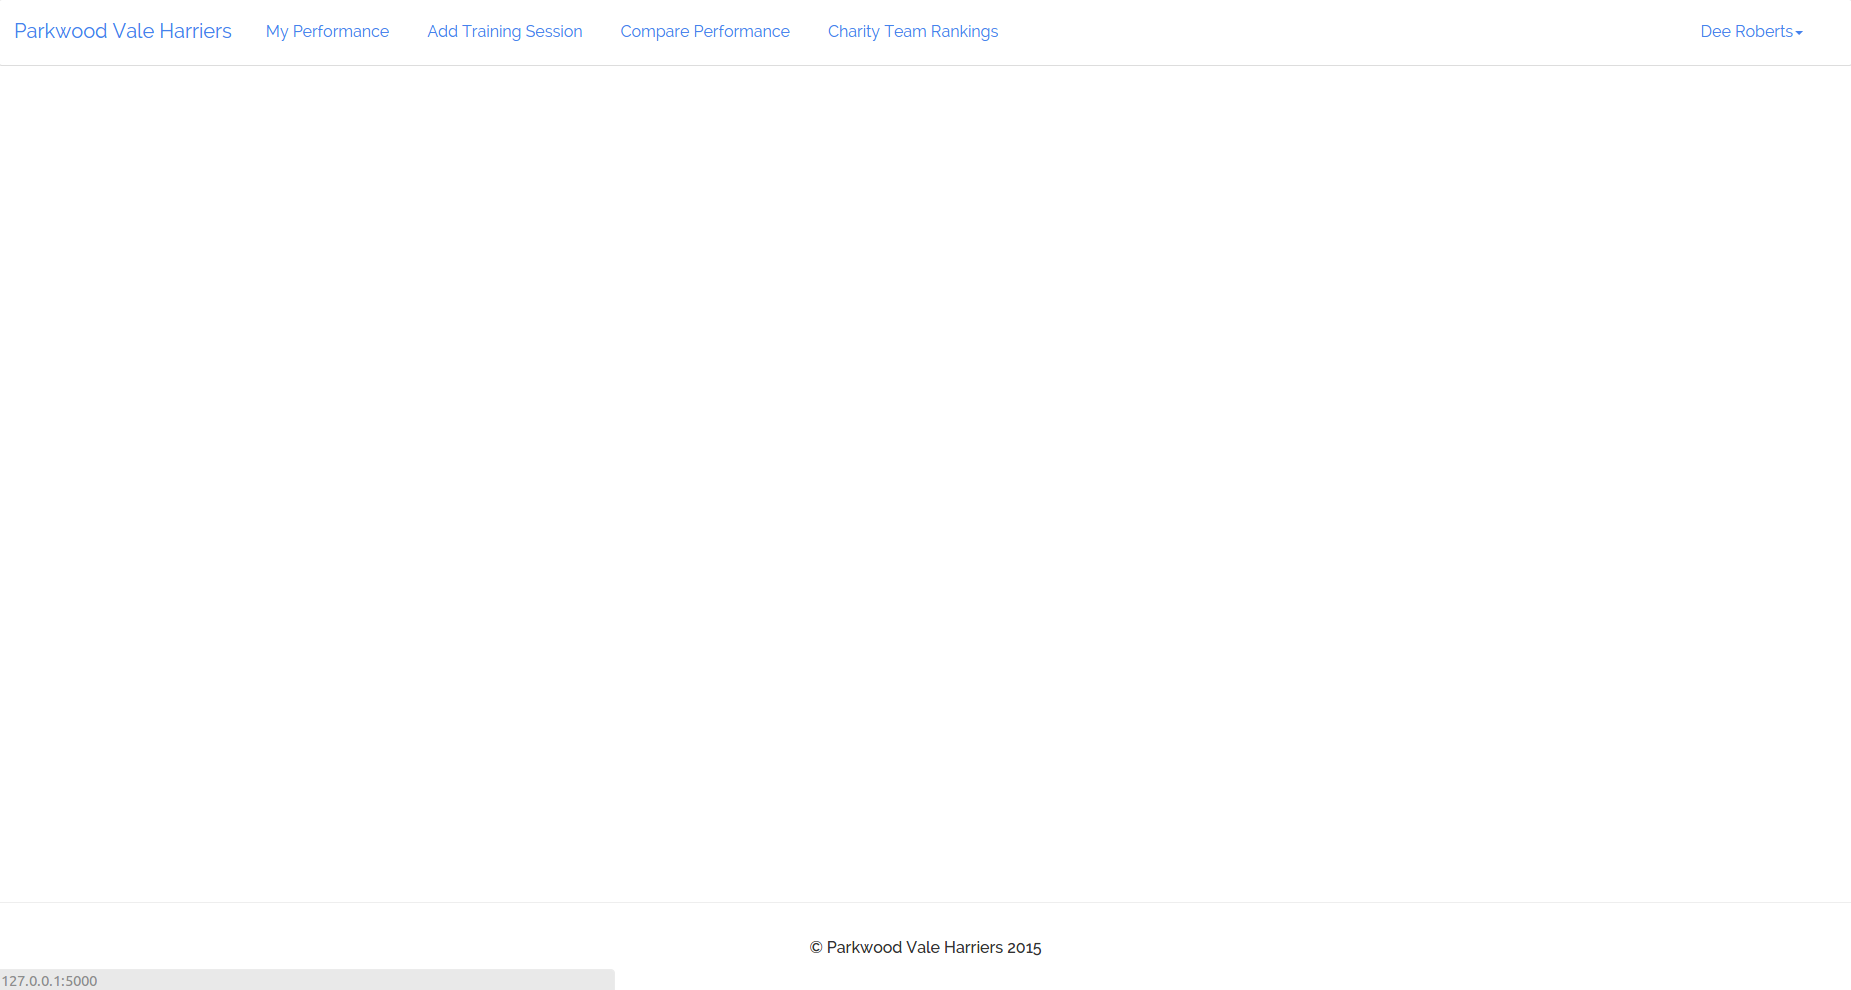
\includegraphics[scale=0.25]{final_ui/layout}
  \caption{Master Layout}
\end{figure}

\clearpage

\subsection{Register Page}
The register page features a clear, simple design, with input boxes laid out in a consistent style. Each input box features placeholder text, to provide a visual guide to runner as to what sort of data they should be typing in. To simplify entry, date of birth input brings up a datepicker widget upon click, making it simple for users to enter their date of birth. Additionally, validation errors are featured at top of page in a big yellow box, making them easy to see; they also have a close button to prevent them getting in way. A link to login page allows users who already have an account to quickly login.

\begin{figure}[h!]
  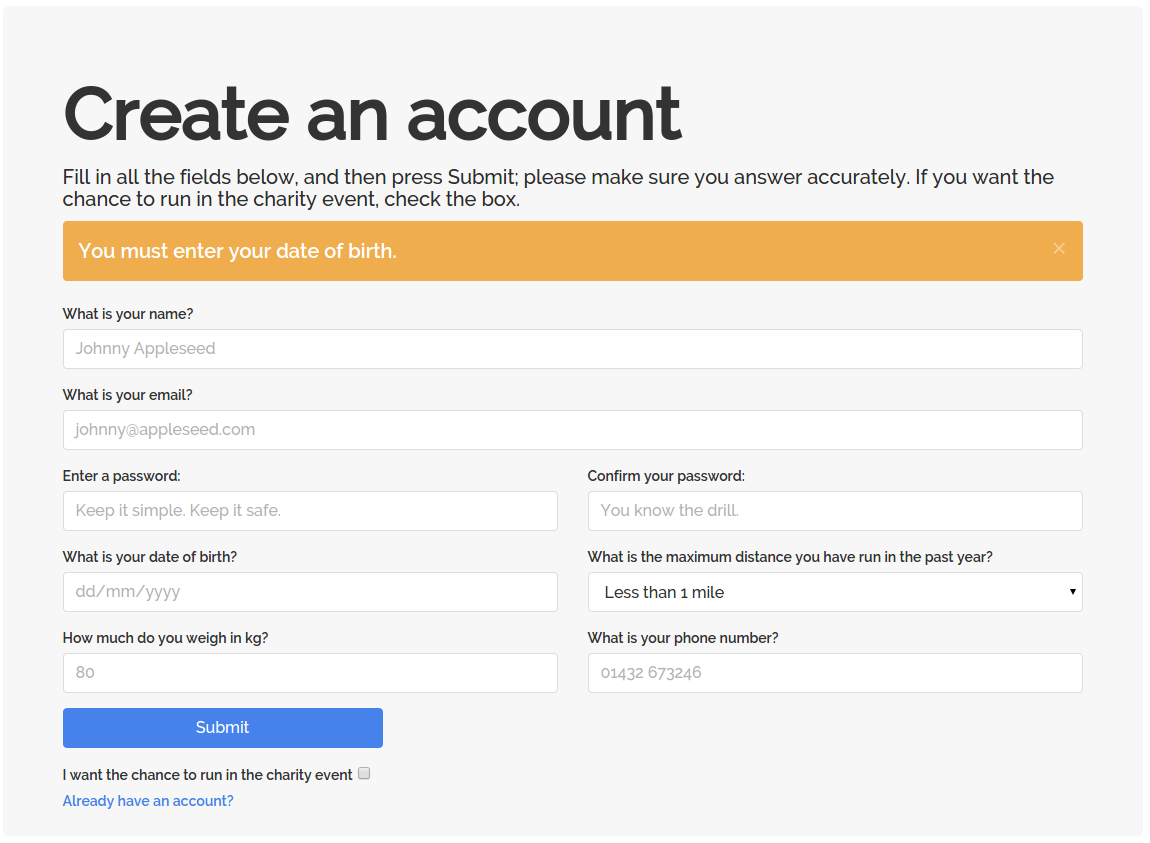
\includegraphics[scale=0.35]{final_ui/register}
  \caption{Registration Page}
\end{figure}
\clearpage

\subsection{Login Page}
As login page has only one function - to get runner logged in to system - it features a very simple layout, with only two input forms and a button. Like registration form, though not visible in this capture, placeholders are overlaid on inputs to provide a visual guide as to should be typed in. Additionally, password field blanks out input, a helpful security measure that prevents onlookers viewing runner's password. For consistency, same validation error system as with registration page is used.

\begin{figure}[h!]
  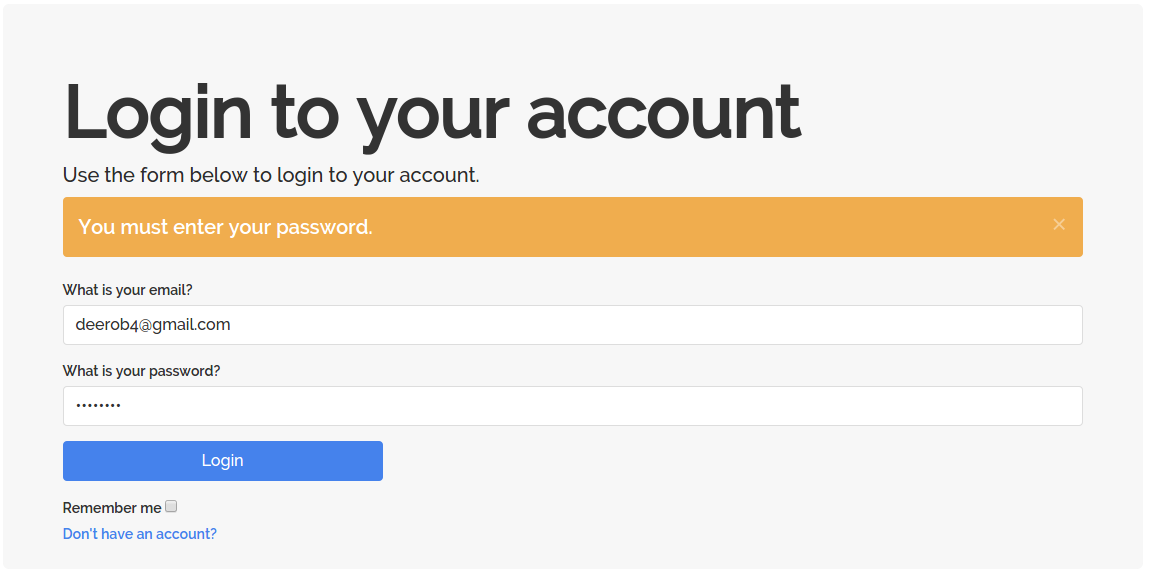
\includegraphics[scale=0.35]{final_ui/login}
  \caption{Login Page}
\end{figure}
\clearpage

\subsection{Profile Page}
The profile page allows runner to view and update their personal information. Certain sections appear on demand, so multiple captures have been taken.

\subsubsection{Main View}
Due to large amount of data that is being presented on this page, a structured approach has been taken, with a three-panel view being implemented. This helps to seperate different areas of page in a logical manner, making it easier for runner to find what they are looking for. Each item of data is given its own row, making it clear which is which. delete account section has been coloured in red, a colour traditionally associated with danger. This helps to convey to runner that bad things will happen if they delete their account. Furthermore, playful text has been used in delete account panel, to bring a sense of amusement and, hopefully, dissuade runner from following through with their actions.

\begin{figure}[h!]
  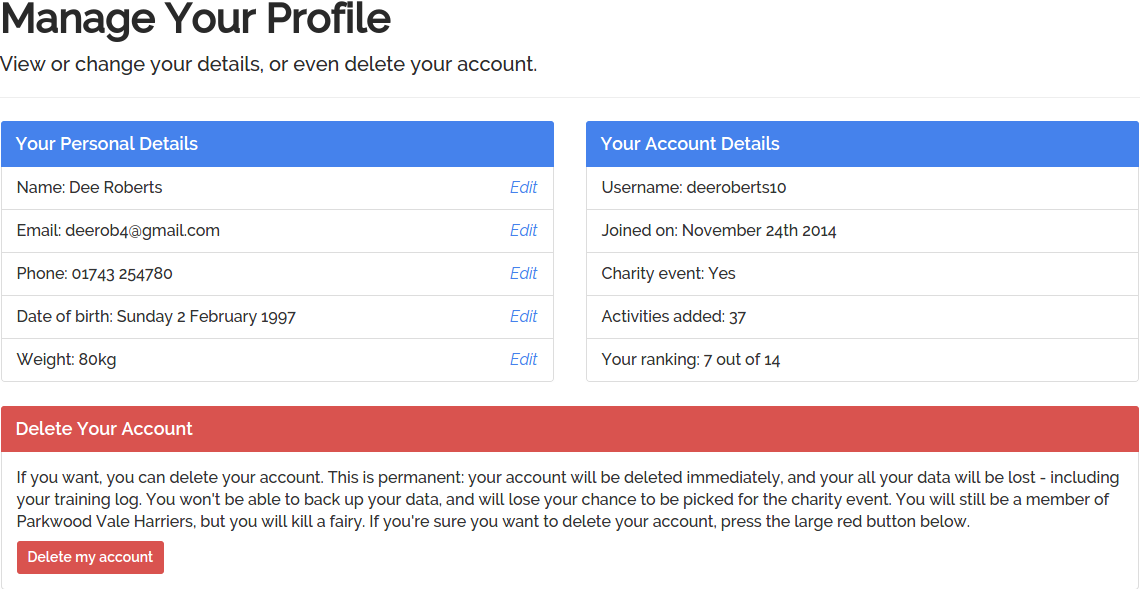
\includegraphics[scale=0.35]{final_ui/profile}
  \caption{Profile Page - Main View}
\end{figure}
\clearpage

\subsubsection{Change Details}
The interface for changing details is very simple - it features just an input for changing element, and a button to confirm. The placeholder text for the input is set to current item, for visual consistency. Making this panel pop up as opposed to being on a seperate page improves flow of page, preventing runner becoming disorientated.

\begin{figure}[h!]
  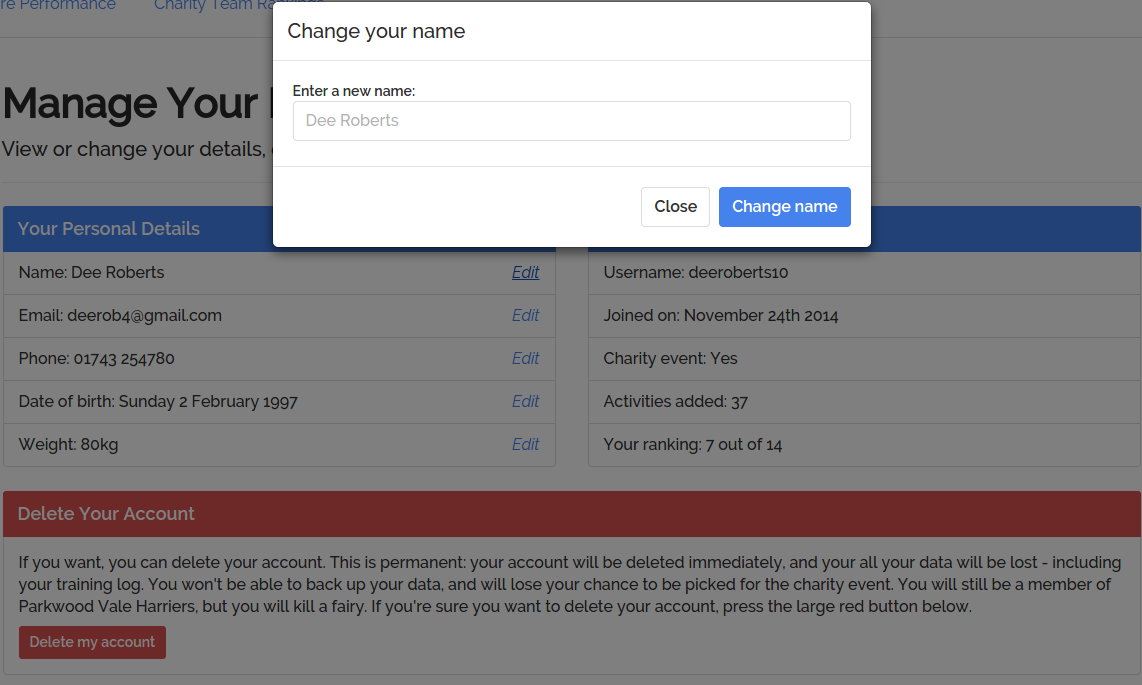
\includegraphics[scale=0.35]{final_ui/profile_change}
  \caption{Profile Page - Change Details}
\end{figure}
\clearpage

\subsubsection{Delete Account}
To ensure that runner is fully aware of severity of deleting their account, they must type in ``I will lose everything'' into box; this also makes it harder for them to accidentally delete their account. Positive reinforcement is used in this section through use of colours - greeen is associated with positivity, and users have been shown to click on green coloured buttons more often than red; this further dissuades them from deleting their account.

\begin{figure}[h!]
  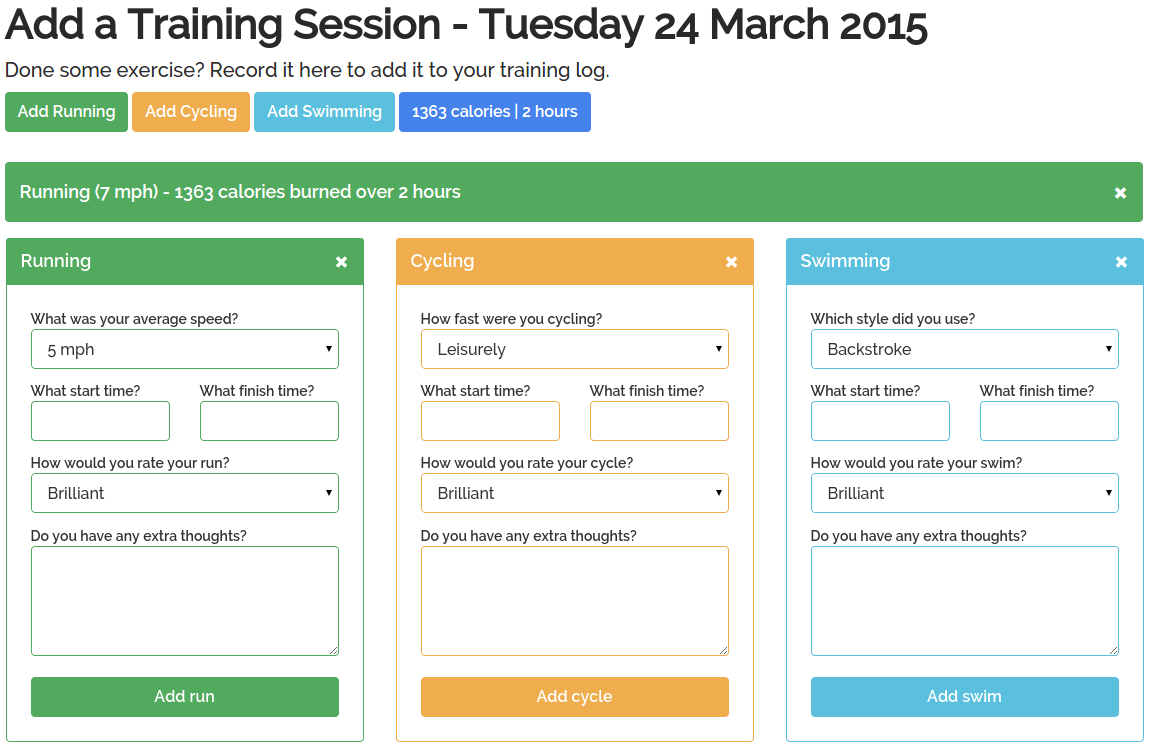
\includegraphics[scale=0.35]{final_ui/account_delete}
  \caption{Profile Page - Delete Account}
\end{figure}
\clearpage

\subsection{Compare Peformance}
Unfortunately, time constraints meant that the implementation of the comparison graphs was never completed, so users are unable to compare their performance. 

\begin{figure}[h!]
  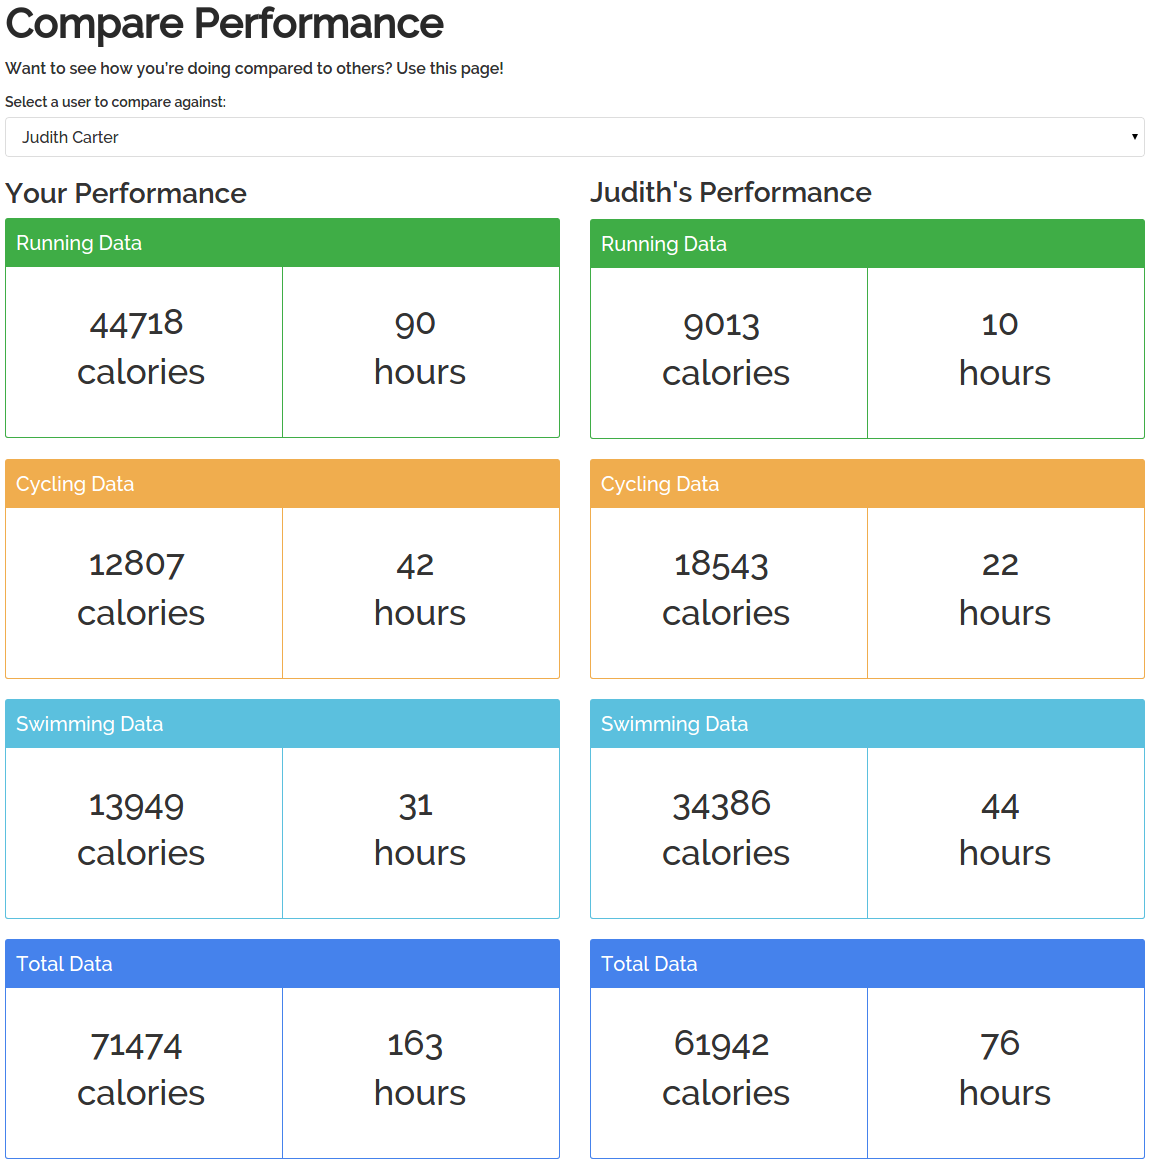
\includegraphics[scale=0.35]{final_ui/compare_performance}
  \caption{Compare Performance Page}
\end{figure}

\clearpage

\subsection{User Performance Page}
The runner performance page is the main page of the system, and is the first page the runner sees when they log into the system.

\begin{figure}[h!]
  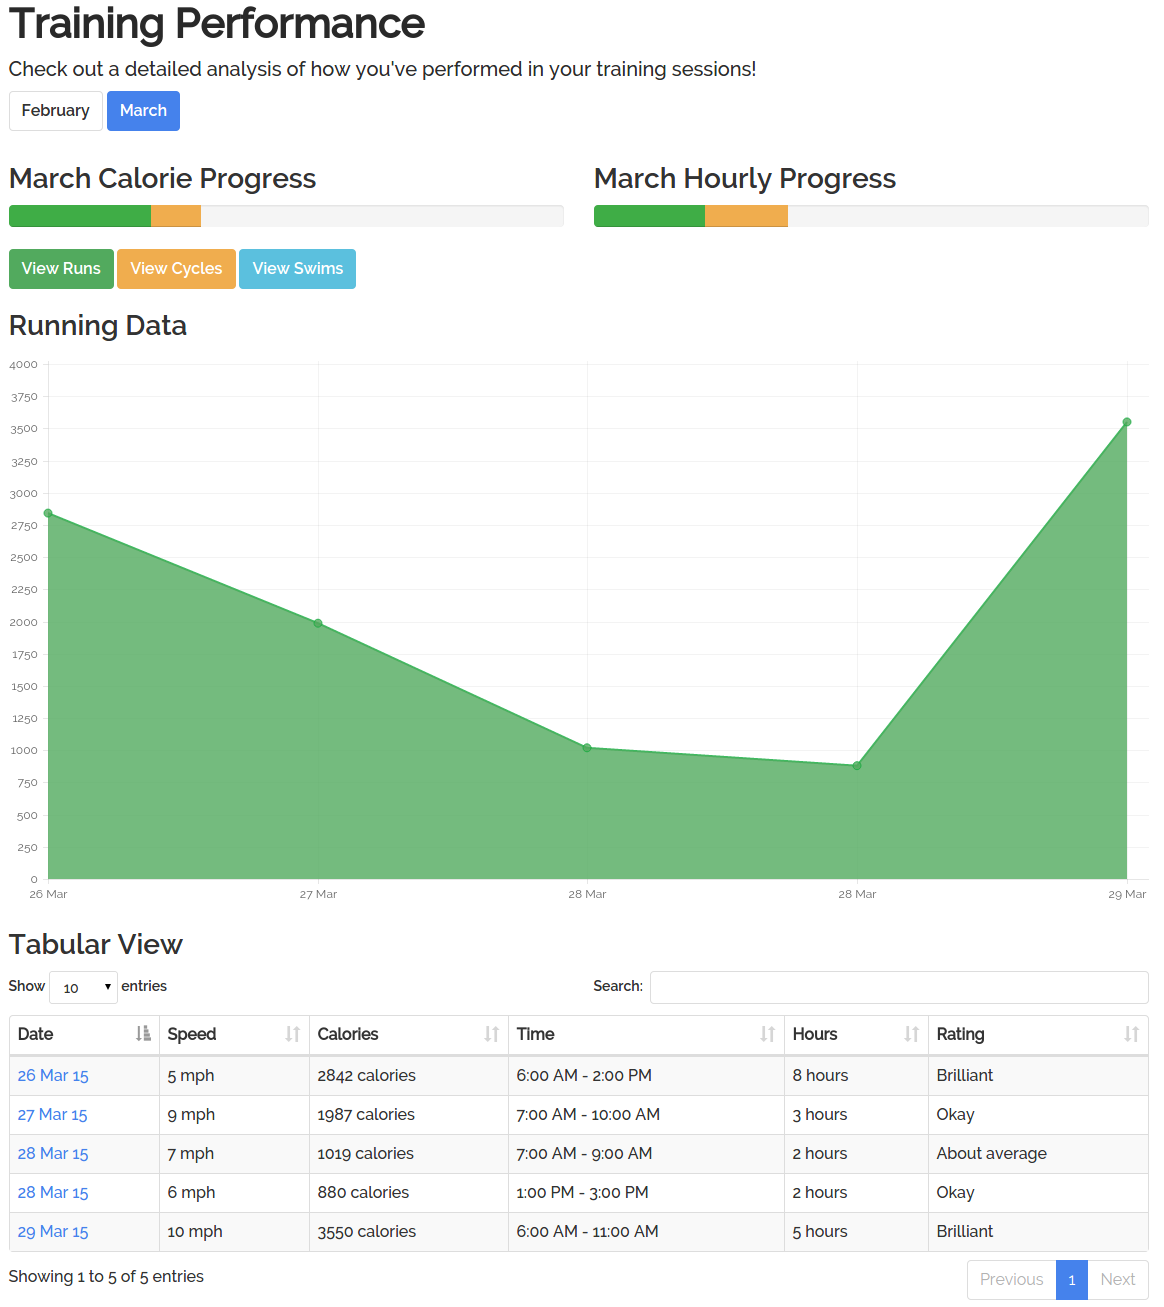
\includegraphics[scale=0.35]{final_ui/user_performance}
  \caption{User Performance Page}
\end{figure}
\clearpage

To prevent the runner being overloaded with data, the performance data is seperated into months, with a different URL for each month - ``/performance/march'' to view performance for March, for example. By default, the runner is automatically taken to the page for the current month, ensuring that they always see the most up to date data. Buttons are available at the top to switch between months; notably, only months where training sessions have been added are visible, ensuring that the runner never sees blank data - something which could be discouraging to the runner.

It allows the runner to view a number of elements relating to their performance in the three sports. The two bars at the top display a simple view of how far the runner is to reaching their goal for the month. The different sports that make up goal progress are shown through colours - green for running, yellow for cycling and blue for swimming, as in the rest of the application. Not shown in the capture are the popups that appear when the runner hovers over the bars - these display the number of calories / hours that make up the bars. 

All of the sessions the runner has done in each sport is plotted on a line chart, allowing for easy visualisation of trends over the month; this makes it very easy for the runner to see how they are doing, a feature that runners would find very helpful When each plot point is moused over, the exact number of calories are shown. There are three different graphs for each sport; these are changed by clicking the colour coded buttons at the top of the graph. When switching sport, the entire section smoothly slides out, allowing the new one to slide in. By providing such a seamless animation, the runner is provided with a sense of place within the system, improving its ease of use.

The page also shows each training session the runner has performed in the selected sport in a table. The table shows all the information about the training session, allowing the runner gain a detailed understanding of how they are progressing - something that is important when training for a charity event. The tables allow for the number of entries shown to be limited, introducing an element of pagination. This allows the runner to control how many sessions they see at once, keeping them orientated within the view. The tables can also be sorted by clicking on the headers, allowing the runner greater control over how they view the sessions; they are listed in date order by default, as the runner would expect.

Additionally, and perhaps most helpfully, the tables allow for the runner to search for specific training sessions. This would be particularly helpful if a runner wished to find all sessions that they rated as brilliant, or all on a particulary day - they would just have to type the term into the search box, and the data is automatically filtered.

\clearpage

\subsection{Add Activity Page}

\begin{figure}[h!]
  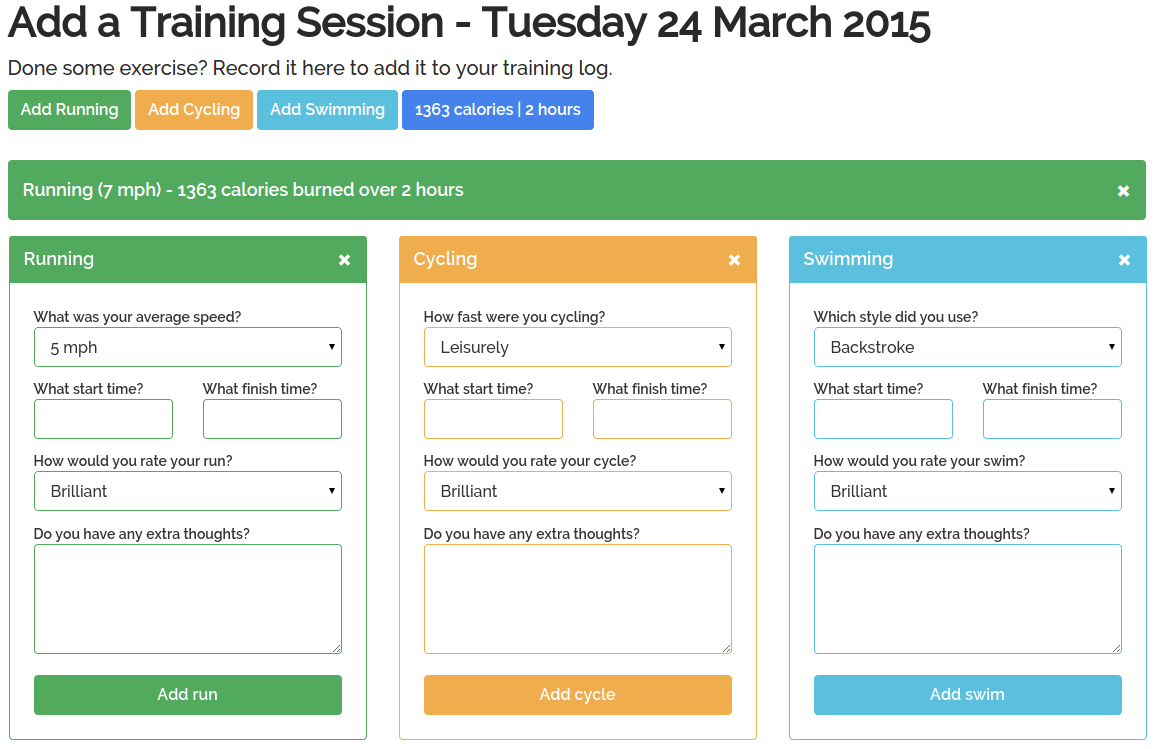
\includegraphics[scale=0.35]{final_ui/add_activity}
  \caption{Add Activity Page}
\end{figure}

\clearpage

\subsection{Rankings Page}

\begin{figure}[h!]
  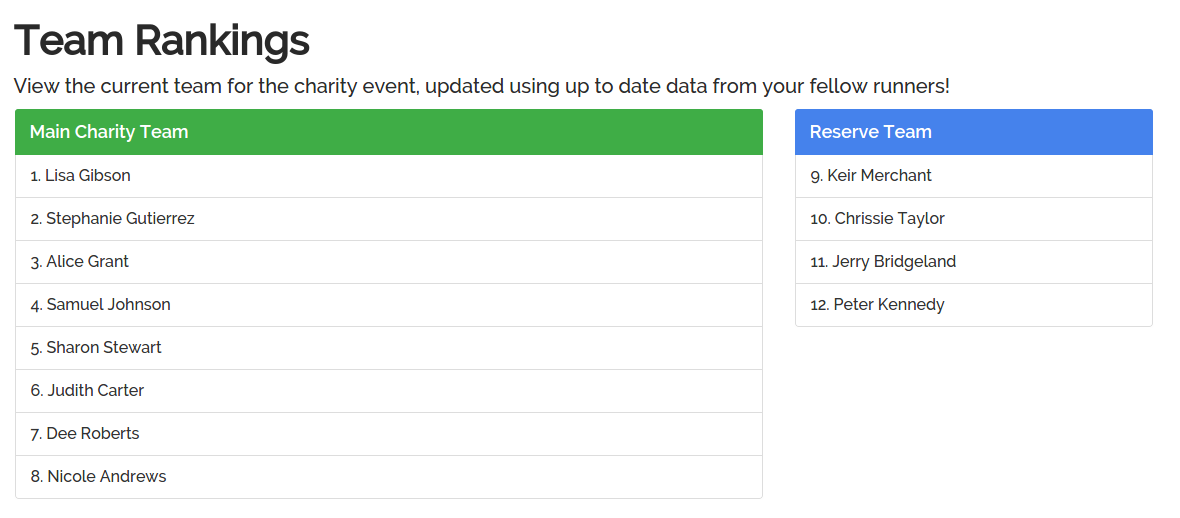
\includegraphics[scale=0.35]{final_ui/rankings}
  \caption{Rankings Page}
\end{figure}

\section{Database Models}
This section contains documentation on finished database tables and models, including an ER diagram showing relationship between tables, schematics, and a visual view.

\subsection{Table Relationships}
The activities and users are linked through a foreign key. This means that there is a one to many relationship between users and activities - one runner can have many activities, but each activity can only have one runner.

\begin{figure}[h!]
  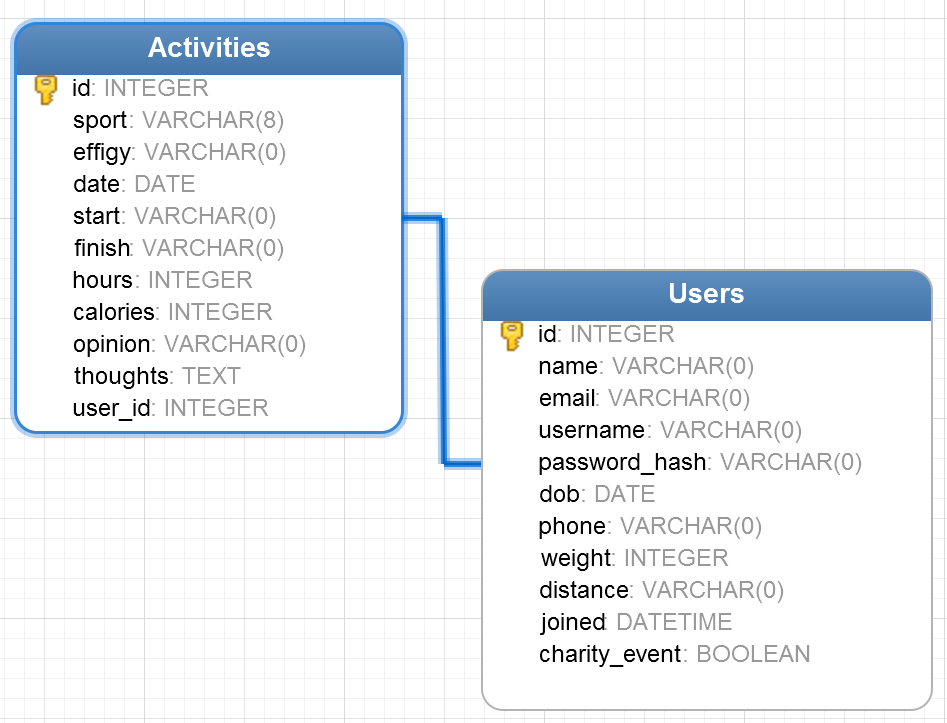
\includegraphics[scale=0.2]{images/database/er_diagram}
  \caption{Table Relationships}
\end{figure}

\clearpage

\subsection{Table Schemas}
Each table in database has its own schema, in which is described name, data type and key type of each column. They can be found below.

\subsubsection{Users Table}
id column is primary key. Email is used to login. Username is used in certain routes; see processes. Weight is used to calculate calories.
\begin{figure}[h!]
  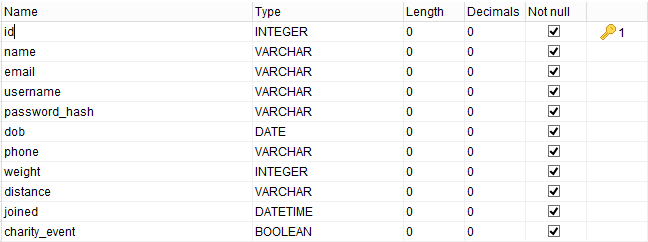
\includegraphics[scale=0.65]{images/database/users_schema}
  \caption{Users Table Schema}
\end{figure}

\subsubsection{Activities Table}
id column is primary key. Effigy is specific details of each activity, such as swimming stroke or running speed. user\_id is foreign key linking activity to a runner.
\begin{figure}[h!]
  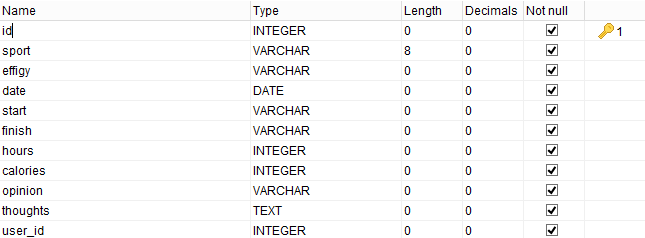
\includegraphics[scale=0.65]{images/database/activities_schema}
  \caption{Activities Table Schema}
\end{figure}

\clearpage

\subsection{Data Views}
following is a snapshot of data in two tables at time of writing, to illustrate how they will appear in production.

\subsubsection{Users Table}
\begin{figure}[h!]
  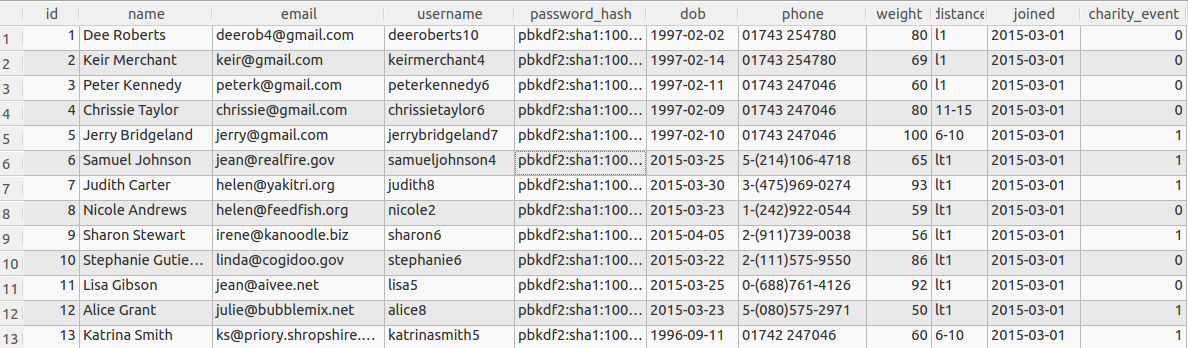
\includegraphics[scale=0.37]{images/database/users_visual}
  \caption{Users Table Data View}
\end{figure}

\subsubsection{Activities Table}
\begin{figure}[h!]
  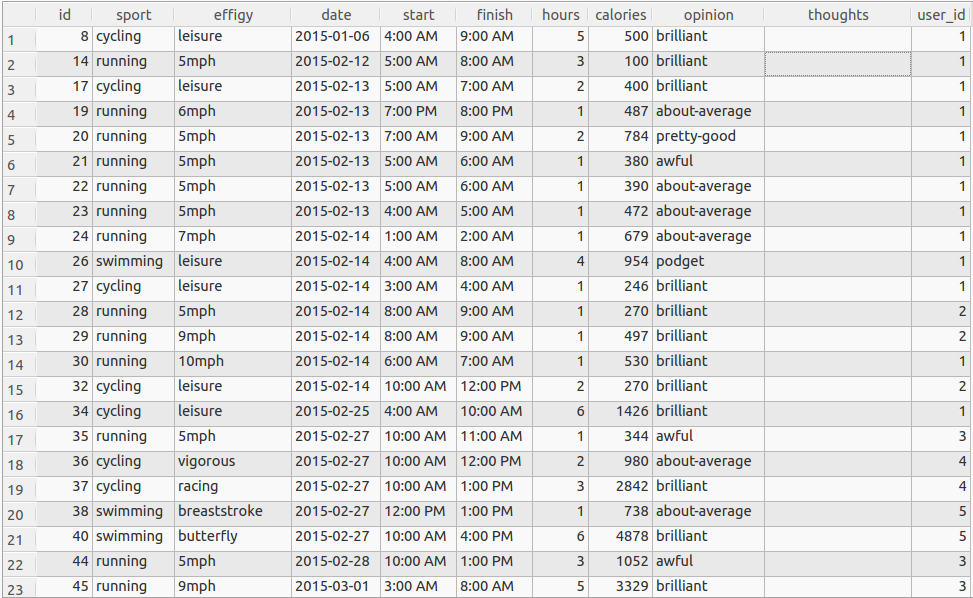
\includegraphics[scale=0.37]{images/database/activities_visual}
  \caption{Activities Table Data View}
\end{figure}

\section{Variables}
A very large number of variables have been used throughout system in order to store data temporarily. It should be noted that variables in Python do not work in same way as in other languages like Visual Basic: a variable acts as a pointer to something already in memory (created by Python automatically), as opposed to creating a space in memory to store contents of variable. Therefore, the code x = 10 merely sets variable x to an address that points at 10, as opposed to writing 10 into memory.

\subsection{Global Variables}
Throughout system, a small number of global variables are used in order to provide functionality. following table lists their names, type and purpose.
\begin{table}[h]
\begin{tabular}{|l|l|l|}
\hline
\textbf{Name} & \textbf{Type} & \textbf{Purpose}                        \\ \hline
login\_manager                    & Object                 & Creates actual Flask application object.     \\ \hline
db                     & Object                 & Returns a connection to database.            \\ \hline
User                   & Object                 & Creates a connection to Users db table.      \\ \hline
Activity               & Object                 & Creates a connection to Activities db table. \\ \hline
current\_user          & Object                 & Returns details about logged in runner.        \\ \hline
\end{tabular}
\caption{Global Variables}
\end{table}

\subsection{Local Variables}
The following table contains a list of all variables used locally throughout the system's functions and classes.
\begin{longtable}{|l|l|l|l|l|}
\hline
\textbf{Name}   & \textbf{Type} & \textbf{File Found} & \textbf{Function}       & \textbf{Purpose}                \\ \hline
name            & Object        & forms.py            & MemberForm              & Creates name input.         \\ \hline
dob             & Object        & forms.py            & MemberForm              & Creates dob input.          \\ \hline
password        & Object        & forms.py            & MemberForm              & Creates password input.     \\ \hline
confirm         & Object        & forms.py            & MemberForm              & Creates confirm input.      \\ \hline
charity\_event  & Object        & forms.py            & MemberForm              & Creates charity input.      \\ \hline
distance        & Object        & forms.py            & MemberForm              & Creates distance input.     \\ \hline
weight          & Object        & forms.py            & MemberForm              & Creates weight input.       \\ \hline
phone           & Object        & forms.py            & MemberForm              & Creates phone input,        \\ \hline
submit          & Object        & forms.py            & MemberForm              & Creates submit button.      \\ \hline
age             & int           & forms.py            & validate\_dob           & Stores runner's age.          \\ \hline
email           & Object        & forms.py            & LoginForm               & Creates email input.        \\ \hline
password        & Object        & forms.py            & LoginForm               & Creates password input.     \\ \hline
remember        & Bool          & forms.py            & LoginForm               & Creates remember input.     \\ \hline
login           & Object        & forms.py            & LoginForm               & Creates login button.       \\ \hline
id              & Object        & models.py           & User                    & Creates id column.          \\ \hline
name            & Object        & models.py           & User                    & Creates name column.        \\ \hline
email           & Object        & models.py           & User                    & Creates email column.       \\ \hline
username        & Object        & models.py           & User                    & Creates username column.    \\ \hline
password\_hash  & Object        & models.py           & User                    & Creates hash column.        \\ \hline
dob             & Object        & models.py           & User                    & Creates dob column.         \\ \hline
phone           & Object        & models.py           & User                    & Creates phone column.       \\ \hline
weight          & Object        & models.py           & User                    & Creates weight column.      \\ \hline
distance        & Object        & models.py           & User                    & Creates distance column.    \\ \hline
joined          & Object        & models.py           & User                    & Creates joined column.      \\ \hline
charity\_event  & Object        & models.py           & User                    & Creates charity column.     \\ \hline
activities      & Object        & models.py           & User                    & Creates relationship property.  \\ \hline
id              & Object        & models.py           & Activity                & Creates id column.          \\ \hline
sport           & Object        & models.py           & Activity                & Creates effigy column.      \\ \hline
date            & Object        & models.py           & Activity                & Creates date column.        \\ \hline
start           & Object        & models.py           & Activity                & Creates start column.       \\ \hline
finish          & Object        & models.py           & Activity                & Creates finish column.      \\ \hline
hours           & Object        & models.py           & Activity                & Creates hours column.       \\ \hline
calories        & Object        & models.py           & Activity                & Creates calories column.    \\ \hline
opinion         & Object        & models.py           & Activity                & Creates opinion column.     \\ \hline
thoughts        & Object        & models.py           & Activity                & Creates thoughts column.    \\ \hline
user\_id        & Object        & models.py           & Activity                & Creates user\_id column.    \\ \hline
today           & Date          & helpers.py          & calculate\_age          & Stores current date.        \\ \hline
months          & List          & perf\_data.py       & perf\_data              & Stores a list of months.        \\ \hline
all\_runs       & Object        & per\_data.py        & perf\_data              & Stores all runner's runs.     \\ \hline
all\_cycles     & Object        & per\_data.py        & perf\_data              & Stores all runner's cycles.   \\ \hline
all\_swims      & Object        & per\_data.py        & perf\_data              & Stores all runner's swims.    \\ \hline
month\_map      & Dict          & per\_data.py        & perf\_data              & Maps months to integers.        \\ \hline
calorie\_goal   & int           & per\_data.py        & perf\_data              & Stores calorie goal.        \\ \hline
hour\_goal      & int           & per\_data.py        & perf\_data              & Stores hourly goal.         \\ \hline
sport             & String      & ajax.py        & sport\_block        & Stores type of sport                \\ \hline
sport             & String      & ajax.py        & send\_activity      & Retrieves sport                     \\ \hline
effiy             & String      & ajax.py        & send\_activity      & Retrieves effigy                    \\ \hline
hours             & int         & ajax.py        & send\_activity      & Retrieves hours                     \\ \hline
start             & int         & ajax.py        & send\_activity      & Retrieves start                     \\ \hline
finish            & int         & ajax.py        & send\_activity      & Retrieves finish                    \\ \hline
opinion           & String      & ajax.py        & send\_activity      & Retrieves opinion                   \\ \hline
thoughts          & String      & ajax.py        & send\_activity      & Retrieves thoughts                  \\ \hline
activity          & Object      & ajax.py        & send\_activity      & Stores completed activity           \\ \hline
activity\_id      & int         & ajax.py        & remove\_activity    & Stores id of activity           \\ \hline
base\_calories    & Dict        & ajax.py        & calculate\_calories & Stores base calorie values          \\ \hline
sport             & String      & ajax.py        & calculate\_calories & Retrieves sport                     \\ \hline
effiy             & String      & ajax.py        & calculate\_calories & Retrieves effigy                    \\ \hline
hours             & int         & ajax.py        & calculate\_calories & Retrieves hours                     \\ \hline
start             & int         & ajax.py        & calculate\_calories & Retrieves start                     \\ \hline
finish            & int         & ajax.py        & calculate\_calories & Retrieves finish                    \\ \hline
opinion           & String      & ajax.py        & calculate\_calories & Retrieves opinion                   \\ \hline
thoughts          & String      & ajax.py        & calculate\_calories & Retrieves thoughts                  \\ \hline
base\_value       & int         & ajax.py        & calculate\_calories & Stores activity base value      \\ \hline
calories          & int         & ajax.py        & calculate\_calories & Stores total calories               \\ \hline
modifier          & int         & ajax.py        & calculate\_calories & Stores calorie modifier     \\ \hline
activity\_data    & Dict        & ajax.py        & calculate\_calories & Stores all activity data            \\ \hline
sport             & String      & ajax.py        & sport\_block        & Stores type of sport                \\ \hline
sport             & String      & ajax.py        & send\_activity      & Retrieves sport                     \\ \hline
effiy             & String      & ajax.py        & send\_activity      & Retrieves effigy                    \\ \hline
hours             & int         & ajax.py        & send\_activity      & Retrieves hours                     \\ \hline
start             & int         & ajax.py        & send\_activity      & Retrieves start                     \\ \hline
finish            & int         & ajax.py        & send\_activity      & Retrieves finish                    \\ \hline
opinion           & String      & ajax.py        & send\_activity      & Retrieves opinion                   \\ \hline
thoughts          & String      & ajax.py        & send\_activity      & Retrieves thoughts                  \\ \hline
activity          & Object      & ajax.py        & send\_activity      & Stores completed activity           \\ \hline
activity\_id      & int         & ajax.py        & remove\_activity    & Stores id of activity           \\ \hline
base\_calories    & Dict        & ajax.py        & calculate\_calories & Stores base calorie values          \\ \hline
sport             & String      & ajax.py        & calculate\_calories & Retrieves sport                     \\ \hline
effiy             & String      & ajax.py        & calculate\_calories & Retrieves effigy                    \\ \hline
hours             & int         & ajax.py        & calculate\_calories & Retrieves hours                     \\ \hline
start             & int         & ajax.py        & calculate\_calories & Retrieves start                     \\ \hline
finish            & int         & ajax.py        & calculate\_calories & Retrieves finish                    \\ \hline
opinion           & String      & ajax.py        & calculate\_calories & Retrieves opinion                   \\ \hline
thoughts          & String      & ajax.py        & calculate\_calories & Retrieves thoughts                  \\ \hline
base\_value       & int         & ajax.py        & calculate\_calories & Stores base value for activity      \\ \hline
calories          & int         & ajax.py        & calculate\_calories & Stores total calories               \\ \hline
modifier          & int         & ajax.py        & calculate\_calories & Stores correct calorie modifier     \\ \hline
activity\_data    & Dict        & ajax.py        & calculate\_calories & Stores all activity data            \\ \hline
month\_map        & Dict        & ajax.py        & user\_charts        & Stores a mapping of months to int       \\ \hline
runs              & Object      & ajax.py        & user\_charts        & Stores all runner's runs              \\ \hline
cycles            & Object      & ajax.py        & user\_charts        & Stores all runner's cycles            \\ \hline
swims             & Object      & ajax.py        & user\_charts        & Stores all runner's swims             \\ \hline
activity\_data    & Dict        & ajax.py        & user\_charts        & Stores chart calories, dates    \\ \hline
month             & String      & ajax.py        & user\_charts        & Stores requested month              \\ \hline
user\_data        & Dict        & ajax.py        & user\_charts        & Stores performance data of runner.    \\ \hline
form              & Object      & auth.py        & register            & Stores instance of MemberForm     \\ \hline
username          & String      & auth.py        & register            & Stores inputted username.           \\ \hline
runner              & Object      & auth.py        & register            & Stores a User object with data          \\ \hline
form              & Object      & auth.py        & login               & Stores instance of LoginForm      \\ \hline
runner              & Object      & auth.py        & login               & Stores details of runner; email       \\ \hline
only\_letters     & String      & main.py        & profiles            & Stores regexp to check name       \\ \hline
valid\_email      & String      & main.py        & profiles            & Stores regexp to check email      \\ \hline
valid\_phone      & String      & main.py        & profiles            & Stores regexp to check phone      \\ \hline
check\_integer    & String      & main.py        & profiles            & Stores regexp to check weight     \\ \hline
activity\_number  & int         & main.py        & profiles            & Stores number of activities of runner \\ \hline
total\_users      & int         & main.py        & profiles            & Stores total number of users        \\ \hline
activities        & Object      & main.py        & add\_training       & Stores all activities for runner on day \\ \hline
total\_calories   & int         & main.py        & add\_training       & Stores total calories done today    \\ \hline
total\_hours      & int         & main.py        & add\_training       & Stores total hours done today       \\ \hline
months            & List        & main.py        & performance         & Stores a list of months             \\ \hline
all\_activities   & Object      & main.py        & performance         & Stores all activities for runner      \\ \hline
available\_months & List        & main.py        & performance         & Stores months runner has sessions in  \\ \hline
users             & Object      & main.py        & compare\_perf       & Stores all users who are charitable \\ \hline
user\_list        & List        & main.py        & compare\_perf       & Stores sorted list of above users   \\ \hline
user\_ranking     & Dict / List & main.py        & rankings            & Stores best running team            \\ \hline
sport             & String      & main.js        & \$sport-click       & Stores requested sport type         \\ \hline
\$start           & Object      & main.js        & validateActivity    & Stores start time input             \\ \hline
\$finish          & Object      & main.js        & validateActivity    & Stores finish time input            \\ \hline
\$activity        & Object      & main.js        & updateActivities    & Stores activity panel               \\ \hline
sport             & String      & main.js        & animateActivity     & Stores session sport                \\ \hline
containerWidth    & int         & main.js        & animateActivity     & Stores width of screen              \\ \hline
start             & Date        & main.js        & calculateHours      & Stores inputted start time          \\ \hline
finish            & Date        & main.js        & calculateHours      & Stores inputted finish time         \\ \hline
effigy            & String      & main.js        & calculateCalories   & Stores effigy of session            \\ \hline
rating            & String      & main.js        & calculateCalories   & Stores rating of session            \\ \hline
start             & String      & main.js        & calculateCalories   & Stores start time of session        \\ \hline
finish            & String      & main.js        & calculateCalories   & Stores finish time of session       \\ \hline
thoughts          & String      & main.js        & calculateCalories   & Stores thoughts of session          \\ \hline
hours             & String      & main.js        & calculateCalories   & Stores hours of session             \\ \hline
caloriesBurned    & int         & main.js        & addActivity         & Stores calories burned by session   \\ \hline
currentCalories   & int         & main.js        & addActivity         & Stores day's current calories       \\ \hline
currentHours      & int         & main.js        & addActivity         & Stores day's current hours          \\ \hline
activityString    & String      & main.js        & addActivity         & Stores string for session           \\ \hline
runningCtx        & Object      & ind\_charts.js & constructChart      & Stores running graph canvas         \\ \hline
swimmingCtx       & Object      & ind\_charts.js & constructChart      & Stores swimming graph canvas        \\ \hline
cyclingCtx        & Object      & ind\_charts.js & constructChart      & Stores cycling graph canvas         \\ \hline
runningData       & Object      & ind\_charts.js & constructChart      & Stores data running graph data      \\ \hline
cyclingData       & Object      & ind\_charts.js & constructChart      & Stores data for cycling graph       \\ \hline
swimmingData      & Object      & ind\_charts.js & constructChart      & Stores data for swimming graph      \\ \hline
runningChart      & Object      & ind\_charts.js & constructChart      & Stores running chart                \\ \hline
cyclingChart      & Object      & ind\_charts.js & constructChart      & Stores cycling chart                \\ \hline
swimmingChart     & Object      & ind\_charts.js & constructChart      & Stores swimming chart               \\ \hline
\caption{Local Variables}
\end{longtable}

\section{Annotated Listings}
This section contains all of code for system, split into several logical categories. The system is made up of a very large number of Python functions, as well as some additional aspects, such as Jinja2 HTML templates to display interface, and CSS to provide styling.

\subsection{HTML Views}
Every page of the system has its own corresponding HTML template. These are used to display data passed by the Python back-end, and provide interface elements such as buttons and dropdown boxes. A comparison can be drawn between them and the XML built by Design Mode in Visual Basic, but, as these also contain some logic of their own, such as for-loops to loop through arrays, it is appropriate to include them in the documentation.

\subsubsection{layout.html}
\lstinputlisting[language=HTML, caption=Main Layout]{../app/templates/layout.html}

\subsubsection{register.html}
\lstinputlisting[language=HTML, caption=Register Page]{../app/templates/auth/register.html}

\subsubsection{login.html}
\lstinputlisting[language=HTML, caption=Login Page]{../app/templates/auth/login.html}

\subsubsection{user\_performance.html}
\lstinputlisting[language=HTML, caption=User Performance Page]{../app/templates/performance/user_performance.html}

\subsubsection{own\_profile.html}
\lstinputlisting[language=HTML, caption=User Profile Page]{../app/templates/profiles/own_profile.html}

\subsubsection{add\_training.html}
\lstinputlisting[language=HTML, caption=Add Session Page]{../app/templates/training/add_training.html}

\subsubsection{compare\_performance.html}
\lstinputlisting[language=HTML, caption=Compare Performance]{../app/templates/performance/compare_performance.html}

\subsubsection{rankings.html}
\lstinputlisting[language=HTML, caption=Rankings Page]{../app/templates/training/rankings.html}

\subsubsection{running\_block.html}
\lstinputlisting[language=HTML, caption=Running Block]{../app/templates/training/running_block.html}

\subsubsection{cycling\_block.html}
\lstinputlisting[language=HTML, caption=Cycling Block]{../app/templates/training/cycling_block.html}

\subsubsection{swimming\_block.html}
\lstinputlisting[language=HTML, caption=Swimming Block]{../app/templates/training/swimming_block.html}


\subsection{JavaScript Functions}
system makes use of some JavaScript in order to create links between front-end (HTML files above) and Python functions. Very little processing is done here; mainly data is transmitted back and forth between client and server.

\subsubsection{main.js}
\lstinputlisting[language=JavaScript, caption=Main JavaScript Functions]{../app/static/js/main.js}

\subsubsection{individual\_charts.js}
\lstinputlisting[language=JavaScript, caption=User Charts]{../app/static/js/individual_charts.js}


\subsection{CSS Styling}
A master CSS file is used to provide styling for system, setting out things like typography, layout and a little animation in places.

\lstinputlisting[caption=main.css]{../app/static/css/main.css}

\subsection{Python Processes}
vast majority of system is written in Python. These function handle everything from connecting and writing to database, to calculating number of calories burned in a session, and everything in between. For a full rundown of what each function does, view processes section.

\subsubsection{\_\_init\_\_.py}
This file handles very low level functions of system, like creating and initialising actual Flask application.
\lstinputlisting[language=Python, caption=\_\_init\_\_.py]{../app/__init__.py}

\subsubsection{forms.py}
This file defines input forms used in login and register pages. It sets validation for each input, and defines appropriate HTML element.
\lstinputlisting[language=Python, caption=forms.py]{../app/forms.py}

\subsubsection{models.py}
This file defines database models used by database. It sets up aspects like foreign/primary keys, and data type of each column.
\lstinputlisting[language=Python, caption=models.py]{../app/models.py}

\subsubsection{helpers.py}
This file defines several smaller helper functions used multiple times throughout system.
\lstinputlisting[language=Python, caption=helpers.py]{../app/helpers.py}

\subsubsection{performance\_data.py}
This file returns a JSON object containing all sessions for a runner in a particular month. It is used throughout system to return data for use in tables and graphs.
\lstinputlisting[language=Python, caption=performance\_data.py]{../app/performance_data.py}

\subsubsection{auth.py}
This file defines routes and processes used in login / register process. They were placed in their own file for efficiency, and because they play a different part to others.
\lstinputlisting[language=Python, caption=auth.py]{../app/controllers/auth.py}

\subsubsection{ajax.py}
This file defines routes used by AJAX calls in JavaScript files. All of these return a value, usually a JSON object, that is then used to dynamically update page.
\lstinputlisting[language=Python, caption=ajax.py]{../app/controllers/ajax.py}

\subsubsection{main.py}
This file defines majority of routes used by system.
\lstinputlisting[language=Python, caption=main.py]{../app/controllers/main.py}

\cleardoublepage


\part{Testing and Evaluation}
This section contains the detailed tests that were performed on the system as it was developed, to ensure that any bugs that existed in the system were caught. Also included is a detailed evaluation of the system.

\subsection{Test Strategy}
I will follow this extensive test strategy to ensure that every part of the system is tested in a thorough manner, thereby increasing the chance that any bugs present in the code are discovered and fixed. For clarity, it has been organised by application page as opposed to process.

\subsubsection{Register Page}
\begin{itemize}
  \item Test that validation on the page works correctly
  \item Test that the database is able to save the new user properly
  \item Test that only users who are logged out can access it
\end{itemize}

\subsubsection{Login Page}
\begin{itemize}
  \item Test that validation on the page works correctly
  \item Test that the login process works properly, with the correct user being logged in
  \item Test that only users who are logged out can access it
\end{itemize}

\subsubsection{Add Training Session}
\begin{itemize}
  \item Test that the correct training cards are added when the appropriate buttons are pressed
  \item Test that the validation on the training cards works properly
  \item Test that the correct number of calories are calculated
  \item Test that the training sessions are saved to the database properly
  \item Test that the training sessions can be deleted from the database
  \item Test that the correct date is shown at the top of the page
\end{itemize}

\subsubsection{Profile Page}
\begin{itemize}
  \item Test that the correct data for the user is shown
  \item Test that the user is able to modify their personal data
  \item Test that the user is able to delete their account
\end{itemize}

\subsubsection{Training Performance}
\begin{itemize}
  \item Test that the graphs for each sport display the correct value
  \item Test that the correct table of training sessions is shown for the user
  \item Test that the only months that have training sessions in are shown to the user
\end{itemize}

\subsubsection{Compare Performance}
\begin{itemize}
  \item Test that the dropdown box is sorted alphabetically and contains only those users who have opted in
  \item Test that the correct data is shown depending on the current user and the other user chosen
\end{itemize}

\subsection{Testing}
The different tests for the different parts of the system have been split up into sections - every test has its own system for organisation.

\subsubsection{Registration Page Validation}
This section tests the validation for the registration page. Most of the inputs on the page have validation to prevent erroneous data being entered, and they are tested here.

\begin{table}[h]
\begin{tabular}{|l|l|l|l|}
\hline
\textbf{Enacted Test}          & \textbf{Expected Action}                  & \textbf{Result} & \textbf{Proof} \\ \hline
Leave name input blank         & Message "you must enter your name"        & As expected.    & Fig1           \\ \hline
Enter 123Dan into name         & Message "name can only have letters"      & As expected.    & Fig2           \\ \hline
Leave email input blank        & Message "you must enter your email"       & As expected.    & Fig3           \\ \hline
Enter danny.com in email       & Message "email must be valid"             & As expected.    & Fig4           \\ \hline
Leave password input blank     & Message "you must enter password"         & As expected.    & Fig5           \\ \hline
Enter abc123 in password field & Message "password must be 8-20 chars"     & As expected.    & Fig6           \\ \hline
Leave date input blank         & Message "you must enter date of birth"    & As expected.    & Fig7           \\ \hline
Leave weight input blank       & Message "you must enter your weight"      & As expected.    & Fig8           \\ \hline
Enter 200 in weight input      & Message "weight must be between 10-100kg" & As expected.    & Fig9           \\ \hline
Leave phone input blank        & Message "you must enter your phone"       & As expected.    & Fig10          \\ \hline
Enter 0123456789 in phone      & Message "phone number must be valid"      & As expected.    & Fig11          \\ \hline
\end{tabular}
\caption{Registration Page Validation}
\end{table}

As can be seen, all of the validation tests passed - they all result in appropriate error messages being shown to the runner, as is written in the processes.

\clearpage

\subsubsection{Login Page Validation}
This section tests the validation for the login page. All of the inputs on this page have validation to prevent erroneous data being entered, and they are tested here.

\begin{table}[h]
\begin{tabular}{|l|l|l|l|}
\hline
\textbf{Enacted Test}                                                                                             & \textbf{Expected Action}                                                                   & \textbf{Actual Result} & \textbf{Proof} \\ \hline
Leave email input blank                                                                                           & \begin{tabular}[c]{@{}l@{}}Error message "you must \\ enter your email"\end{tabular}       & As expected.           & Fig12           \\ \hline
Enter danny.com in email                                                                                          & \begin{tabular}[c]{@{}l@{}}Error message "your email \\ must be valid"\end{tabular}        & As expected.           & Fig13           \\ \hline
Leave password input blank                                                                                        & \begin{tabular}[c]{@{}l@{}}Error message "you must \\ enter your password"\end{tabular}    & As expected.           & Fig14           \\ \hline
\begin{tabular}[c]{@{}l@{}}Enter john@smith.com in\\ email input and abc123def \\ in password input.\end{tabular} & \begin{tabular}[c]{@{}l@{}}Error message "invalid\\ email / password entered"\end{tabular} & As expected.           & Fig15           \\ \hline
\end{tabular}
\caption{Login Page Validation}
\end{table}

As can be seen, all of the validation tests passed - they all result in appropriate error messages being shown to the runner, as is written in the processes. Additionally, the system correctly identifies if a runner enters an incorrect email or password, an important security feature.

\subsubsection{Registering User to Database}
This section tests that the registration page actually works, and the runner is successfully added to the database with all the correct data.\\

{\setlength{\parindent}{0cm}
Navigate to the registration page, and fill in the inputs as follows:
\begin{description}[labelindent=1cm]
  \item[Name Input:] Katrina Smith
  \item[Email Input:] katrina@gmail.com
  \item[Password Input:] pythonisdifficult
  \item[Password Confirm:] pythonisdifficult
  \item[DOB Input:] 06/03/1951
  \item[Maximum Distance:] 11 - 15 miles
  \item[Weight Input:] 56kg
  \item[Phone Number Input:] 01743 548397
  \item[Charity Event:] True (ticked)
\end{description}
}

\clearpage

When the submit button is pressed, a new runner should be added to the Users table with these parameters. The username field should be set to \textit{katrinasmith} and a random number between 1 and 10, and the joined field should be set to the date the test was performed. Additionally, the password\_hash field should contain an encrypted version of the string \textit{pythonisdifficult}. This is the Users table before the test was run:

\begin{figure}[h!]
  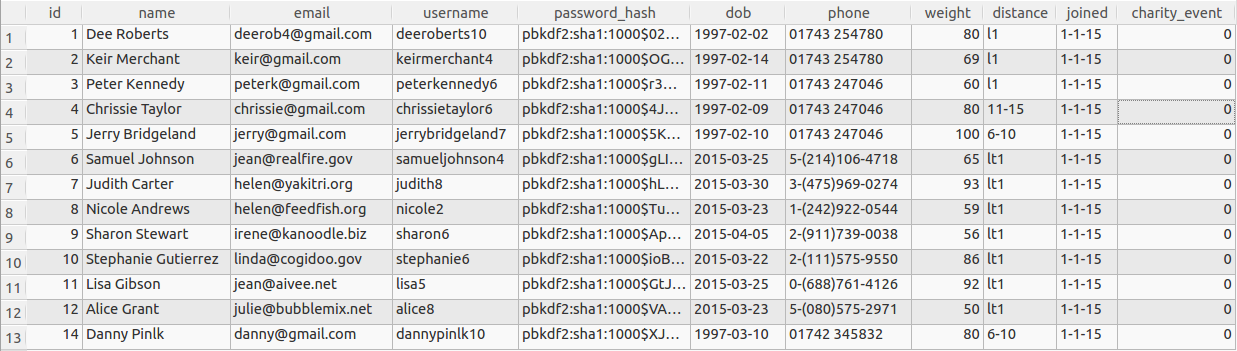
\includegraphics[scale=0.35]{images/testing/add_user/database_before}
  \caption{Users Table Before Test}
\end{figure}

And this is the table afterwards (new runner highlighted):

\begin{figure}[h!]
  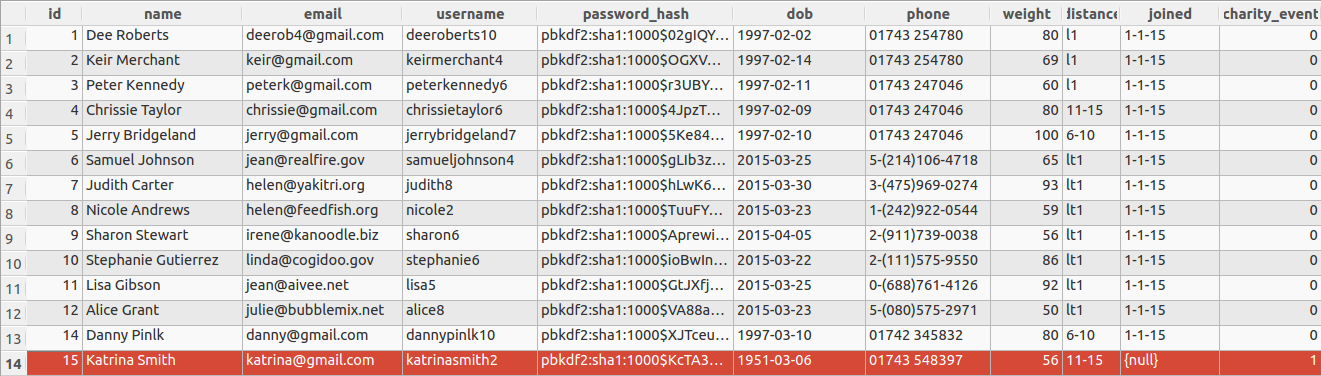
\includegraphics[scale=0.34]{images/testing/add_user/database_after_broken}
  \caption{Users Table After Test}
\end{figure}

\clearpage

As is clear, the test succeeded in every regard but the storage of the \textit{joined} field, which was set to \textit{null}. This was because the datatype for the column in models.py had been set to \textit{DateTime} as opposed to \textit{Date}, as shown here:

\begin{figure}[h!]
    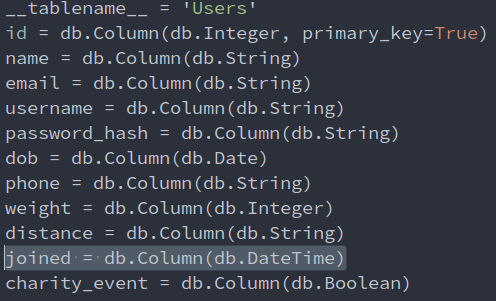
\includegraphics[scale=0.5]{images/testing/add_user/code_before}
    \caption{models.py before modification}
\end{figure}

It was replaced with this:

\begin{figure}[h!]
    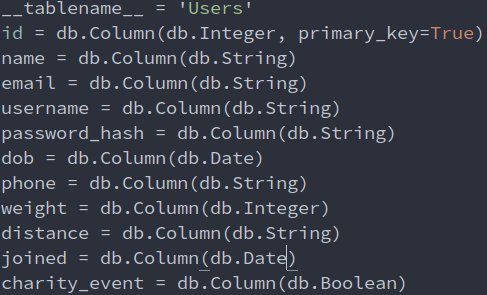
\includegraphics[scale=0.5]{images/testing/add_user/code_after}
    \caption{models.py after modification}
\end{figure}

This fixed the issue; entire section works perfectly now:

\begin{figure}[h!]
    
\includegraphics[scale=0.33]{images/testing/add_user/database_fixed}
    \caption{Fixed Users Table}
\end{figure}

\subsubsection{Navigation Bar}
This section tests that the navigation bar works correctly, with the correct links pointing to the correct areas; likewise, the two different navigation bars are differentiated, as the links change depending on whether the user is logged in or not.

\begin{table}[h]
\begin{tabular}{|l|l|l|l|}
\hline
\multicolumn{1}{|c|}{\textbf{Navigation Link}} & \multicolumn{1}{c|}{\textbf{Expected URL}} & \multicolumn{1}{c|}{\textbf{Visible When}} & \multicolumn{1}{c|}{\textbf{Signature}} \\ \hline
My Performance                                 & /performance/current\_month                & Logged in                                  &                                                 \\ \hline
Add Training                                   & /add-training                              & Logged in                                  &                                                 \\ \hline
Compare Performance                            & /performance/compare                       & Logged in                                  &                                                 \\ \hline
Charity Team Rankings                          & /rankings                                  & Logged in                                  &                                                 \\ \hline
Your Profile                                   & /profile/username                          & Logged in                                  &                                                 \\ \hline
Logout                                         & /logout                                    & Logged in                                  &                                                 \\ \hline
Register                                       & /register                                  & Logged out                                 &                                                 \\ \hline
Login                                          & /login                                     & Logged out                                 &                                                 \\ \hline
\end{tabular}
\end{table}

It would be impossible to show that the navigation works effectively through screenshots, so a column has been added for a suitable figure of authority to testify that all is as it should be. Screenshots below show the two different navigation bar states; they work perfectly, as described above in the \textit{Visible When} column:

\begin{figure}[h!]
    
\includegraphics[scale=0.33]{images/testing/navigation/logged_in}
    \caption{Navigation When Logged In}
\end{figure}

\begin{figure}[h!]
    
\includegraphics[scale=0.40]{images/testing/navigation/logged_out}
    \caption{Navigation When Logged Out}
\end{figure}

\clearpage


\subsubsection{Adding Training Session to Database}
This section tests the system's ability to add training sessions to the database. Log in as Katrina Smith:
\begin{description}[labelindent=1cm]
  \item[Email address:] katrina@gmail.com
  \item[Password:] pythonisdifficult
\end{description}

{\setlength{\parindent}{0cm}
Navigate to the Add Session page, and click the green Add Run button. Fill in the details as follows:
\begin{description}[labelindent=1cm]
  \item[Average Speed:] 7mph
  \item[Start Time:] 13:00pm
  \item[Finish Time:] 15:00pm
  \item[Rating:] Pretty good
  \item[Extra Thoughts:] I liked it. It was very fun. No no?
\end{description}
The box should look like this:
\begin{figure}[h!]
    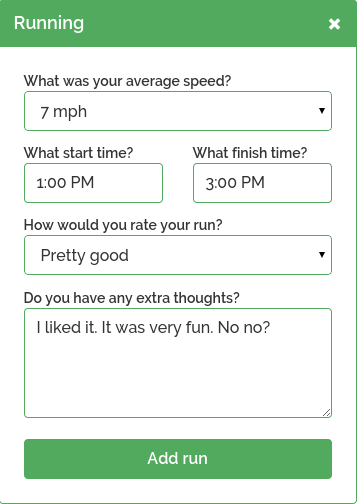
\includegraphics[scale=0.33]{images/testing/add_activity/activity_box}
    \caption{Fixed Users Table}
\end{figure}
}

\clearpage

This is the Activities table before the test was run:
\begin{figure}[h!]
    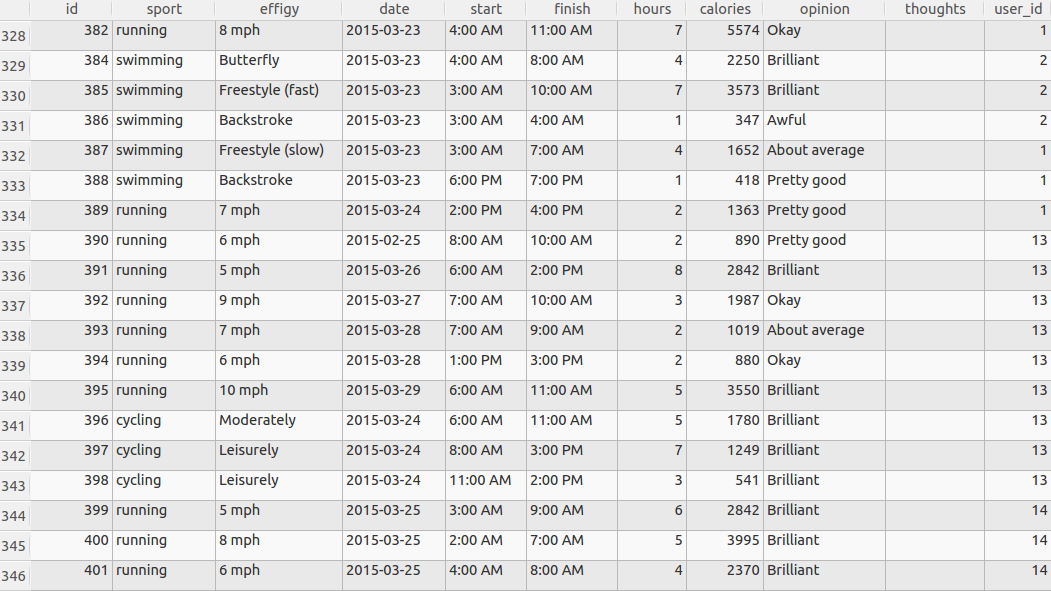
\includegraphics[scale=0.33]{images/testing/add_activity/database_before}
    \caption{Activities Table Before}
\end{figure}

This is the Activities table after the test was run:
\begin{figure}[h!]
    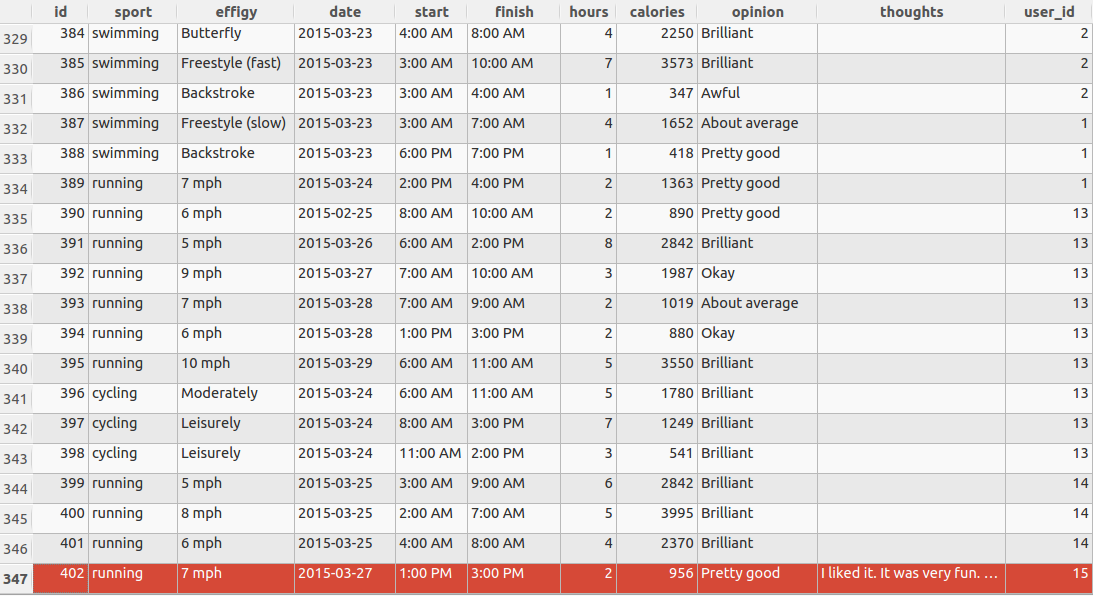
\includegraphics[scale=0.33]{images/testing/add_activity/database_after}
    \caption{Activities Table After}
\end{figure}

As can be seen, the activity was added perfectly; the test succeeded.

\clearpage

\subsubsection{Delete User}
This section tests the system's ability to delete the runner. Log in as Katrina Smith:
\begin{description}[labelindent=1cm]
  \item[Email address:] katrina@gmail.com
  \item[Password:] pythonisdifficult
\end{description}
Navigate to the profile page and press the ``Delete my account'' button. Type ``I will lose everything'' into the box and press the ``Delete account'' button:

\begin{figure}[h!]
    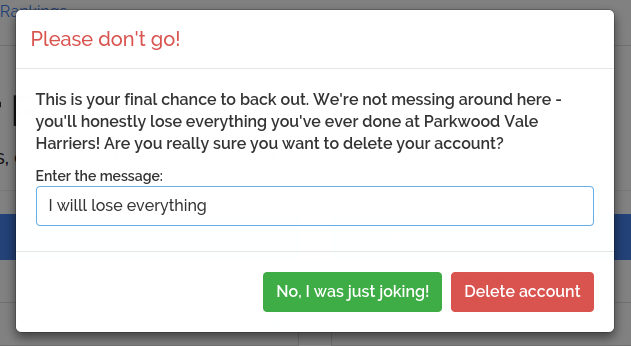
\includegraphics[scale=0.33]{images/testing/delete_user/panel}
    \caption{Delete User Panel}
\end{figure}

You should be redirected to the login page with a message saying ``Your account has been delete. Sorry to see you go!'' and the runner should be removed from the Users Table. All their activities should be removed.

This is the Users table before the test:

\begin{figure}[h!]
    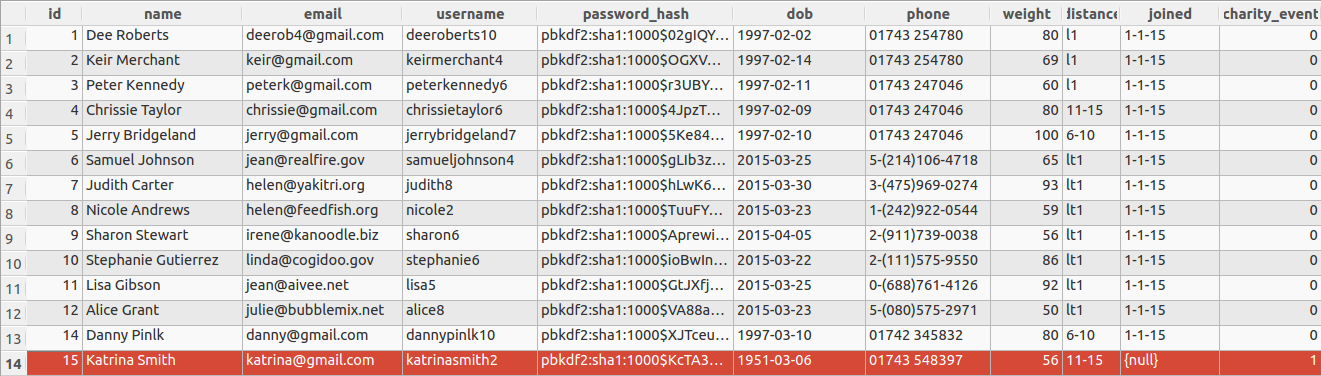
\includegraphics[scale=0.33]{images/testing/add_user/database_after_broken}
    \caption{Users Table before Test}
\end{figure}

\clearpage

And this is the Users table after the test:

\begin{figure}[h!]
    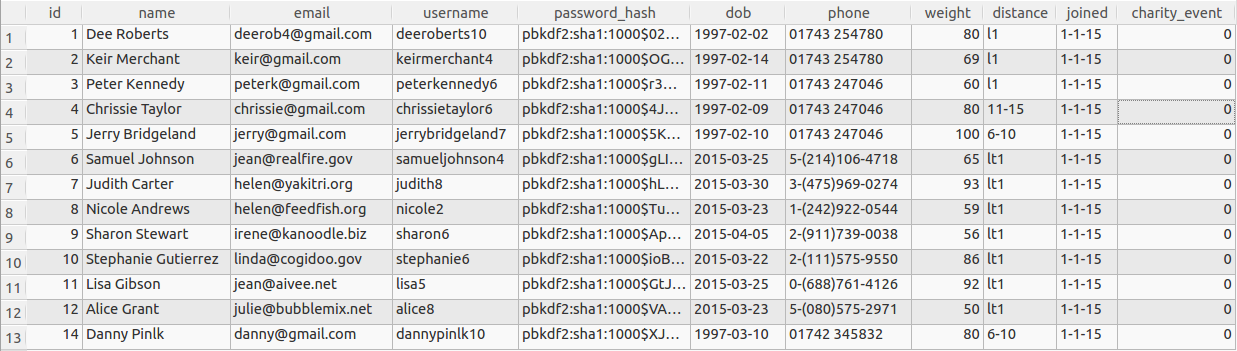
\includegraphics[scale=0.33]{images/testing/add_user/database_before}
    \caption{Users Table after Test}
\end{figure}

The redirect and message also worked:

\begin{figure}[h!]
    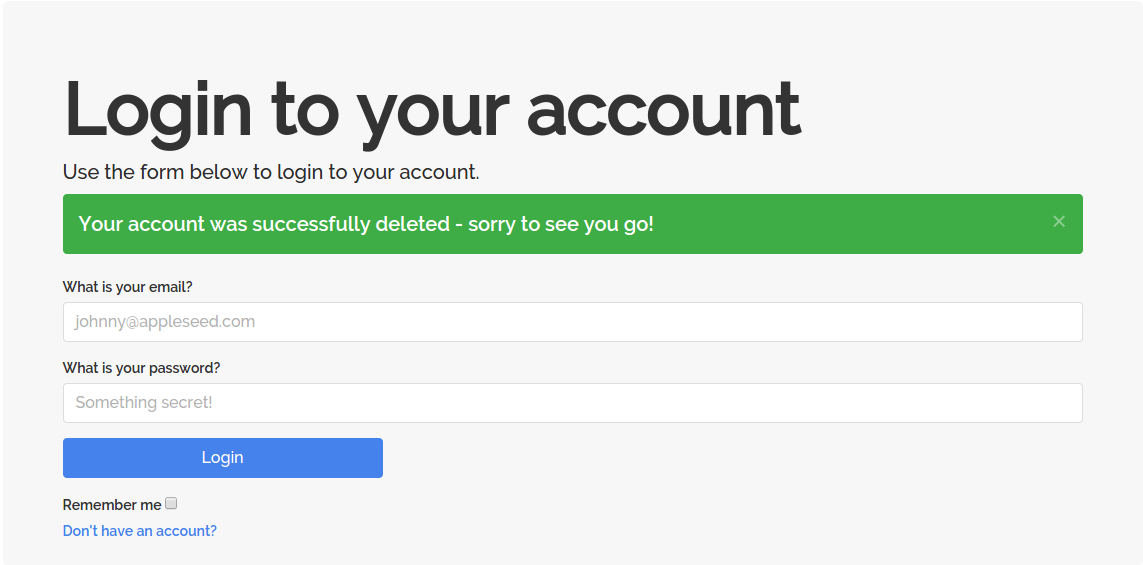
\includegraphics[scale=0.33]{images/testing/delete_user/sorry}
    \caption{Redirected to login screen after account delete}
\end{figure}

As can be seen, the runner was deleted perfectly; the test succeeded.

\clearpage

\subsubsection{User Performance Graphs}
This section tests that the performance graphs work properly, and display the correct data.\\

{\setlength{\parindent}{0cm}
Create three new members, with the following details:

\begin{framed}
Name: Peter Kennedy | Email: peterk@gmail.com | D.O.B: 02/03/1956 | Max distance: Less than 1 mile | Weight: 60kg | Phone Number: 01742247845 | Charity event: false
\end{framed}

\begin{framed}
Name: Chrissie Taylor | Email: chrissie@gmail.com | D.O.B: 01/09/1951 | Max distance:  1-5 miles | Weight: 80kg | Phone Number: 01742247845 | Charity event: true
\end{framed}

\begin{framed}
Name: Jerry Bridgeland | Email: jezzab@gmail.com | D.O.B: 01/09/1951 | Max distance:  11-15 miles | Weight: 100kg | Phone Number: 01742247845 | Charity event: true
\end{framed}

Now add the following training sessions:

\begin{framed}
For Peter Kennedy, do not add any training sessions.
\end{framed}

\begin{framed}
For Chrissie Taylor, add the following training sessions:\\\\
Sport: Cycling | Start Time: 10:00am | Finish time: 12:00am | Speed: vigorously | Rating: average\\\\
Sport: Cycling | Start Time: 10:00am | Finish time: 16:00am | Speed: racing | Rating: brilliant\\\\
Sport: Cycling | Start Time: 10:00am | Finish time: 13:00am | Speed: racing | Rating: brilliant
\end{framed}

\begin{framed}
For Jerry Bridgeland, add the following training sessions:\\\\
Sport: Swimming | Start Time: 10:00am | Finish time: 12:00am | Speed: backstroke | Rating: average\\\\
Sport: Swimming | Start Time: 10:00am | Finish time: 16:00am | Speed: breaststroke | Rating: brilliant\\\\
Sport: Swimming | Start Time: 10:00am | Finish time: 12:00am | Speed: butterfly | Rating: okay\\\\
Sport: swimming | Start Time: 09:00am | Finish time: 11:00am | Speed: backstroke | Rating: awful\\\\
Sport: Swimming | Start Time: 10:00am | Finish time: 13:00am | Speed: backstroke | Rating: brilliant
\end{framed}

Peter's graph should contain no data.

\begin{figure}[h!]
    
\includegraphics[scale=0.33]{images/testing/graphs/peter}
    \caption{Peter Kennedy's Graph}
\end{figure}

\clearpage

Chrissie's graph sould contain three data points with connecting lines.

\begin{figure}[h!]
    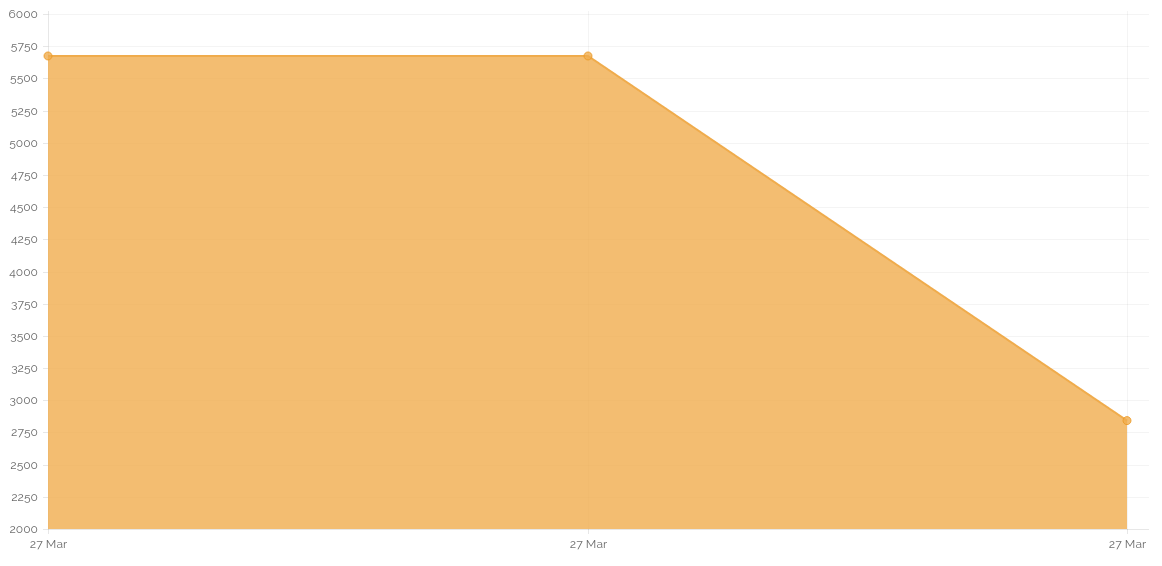
\includegraphics[scale=0.33]{images/testing/graphs/chrissie}
    \caption{Chrissie Taylor's Graph}
\end{figure}

\clearpage

Jerry's graph should contain five data points with connecting lines.

\begin{figure}[h!]
    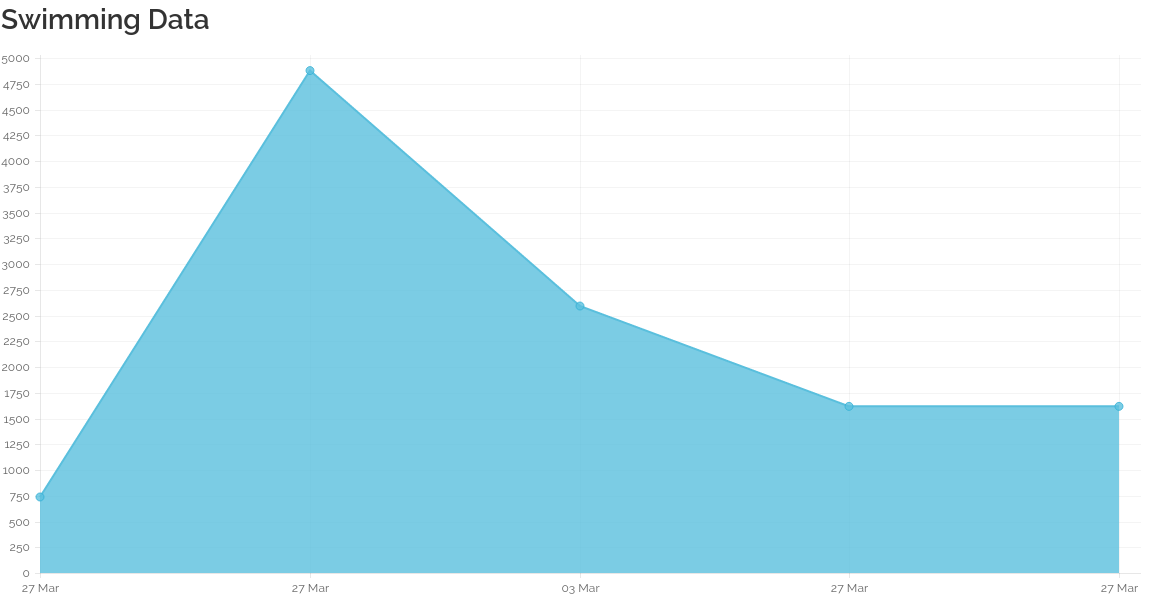
\includegraphics[scale=0.33]{images/testing/graphs/jerry}
    \caption{Jerry Bridgeland's Graph}
\end{figure}

\clearpage

\subsubsection{Calorie Calculation}
Create a runner with a weight of 87kg. Add a running session with the following parameters:

\begin{description}[labelindent=1cm]
  \item[Speed:] 8 mph
  \item[Start time:] 12 PM
  \item[Finish time:] 3:00 PM
  \item[Rating:] Pretty good
\end{description}

It should look like this:

\begin{figure}[h!]
    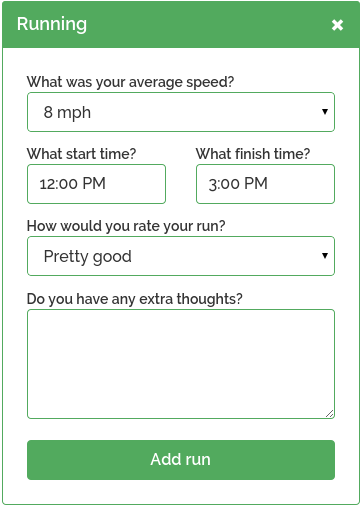
\includegraphics[scale=0.33]{images/testing/calorie/running}
    \caption{Running Block}
\end{figure}

The session is worth 2602 calories. This should be reflected in the system. It was, as shown here:

\begin{figure}[h!]
    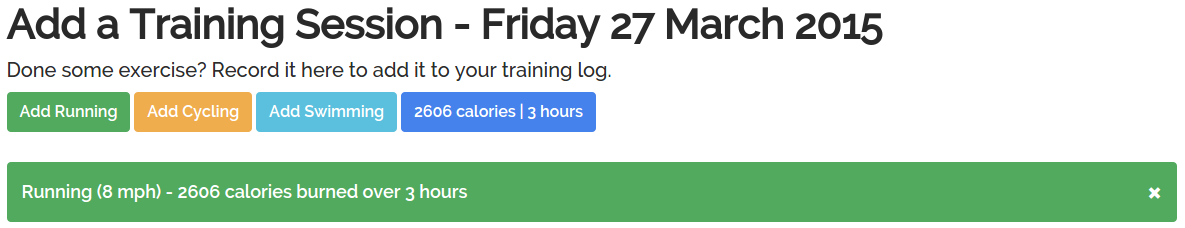
\includegraphics[scale=0.33]{images/testing/calorie/finished}
    \caption{Correct Calorie Calculation}
\end{figure}

\subsubsection{Profile Page - Viewing Data}
This section tests that the correct information is displayed on the runner's profile page, according to the runner that is logged in.\\

Login as Peter Kennedy:

\begin{description}[labelindent=1cm]
  \item[Email:] peterk@gmail.com
  \item[Password:] 70153590
\end{description}

The profile page personal details should look as follows:

\begin{description}[labelindent=1cm]
  \item[Name:] Peter Kennedy
  \item[Email:] peterk@gmail.com
  \item[Phone:] 01743 247046
  \item[Date of birth:] Tuesday 11 February 1997
  \item[Weight:] 60kg
\end{description}

The account details page should look as follows:

\begin{description}[labelindent=1cm]
  \item[Username:] peterkennedy6
  \item[Joined on:] January 16th 2015
  \item[Charity event:] No
  \item[Activities added:] \textit{variable}
  \item[Your ranking:] \textit{variable}
\end{description}

As can be seen, the data displays perfectly:

\begin{figure}[h!]
    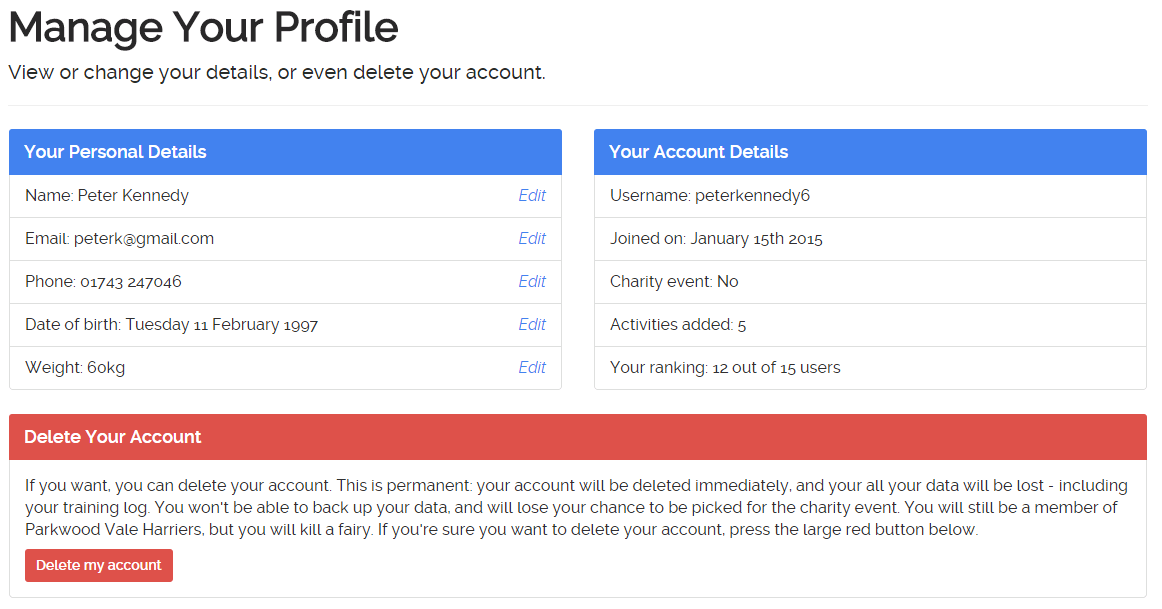
\includegraphics[scale=0.5]{images/testing/profile/working_profile}
    \caption{Working Profile Page}
\end{figure}

\clearpage

\subsubsection{Profile Page - Updating Data}
This section tests that the user's data can be updated successfully, using the Edit buttons and modals provided by each element.\\

Login as Peter Kennedy:

\begin{description}[labelindent=1cm]
  \item[Email:] peterk@gmail.com
  \item[Password:] 70153590
\end{description}

Click the Edit button on the side of the name field. Type in "Dave Ellis" into the name box, and press the "Change name" button. The box should look like this:

\begin{figure}[h!]
    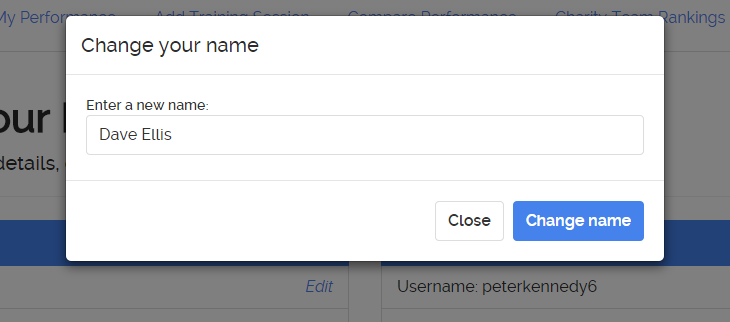
\includegraphics[scale=0.33]{images/testing/profile/change_name}
    \caption{Change Name Box}
\end{figure}

After the button is pressed, the page should refresh, and a green message should appear saying "Your name has been successfully changed." Likewise, the name shown in the Name box should also have been modified to Dave Ellis, and the username should have been changed to "daveellis", and then a random number from 1 - 10. As can be seen, the test ran perfectly:

\begin{figure}[h!]
    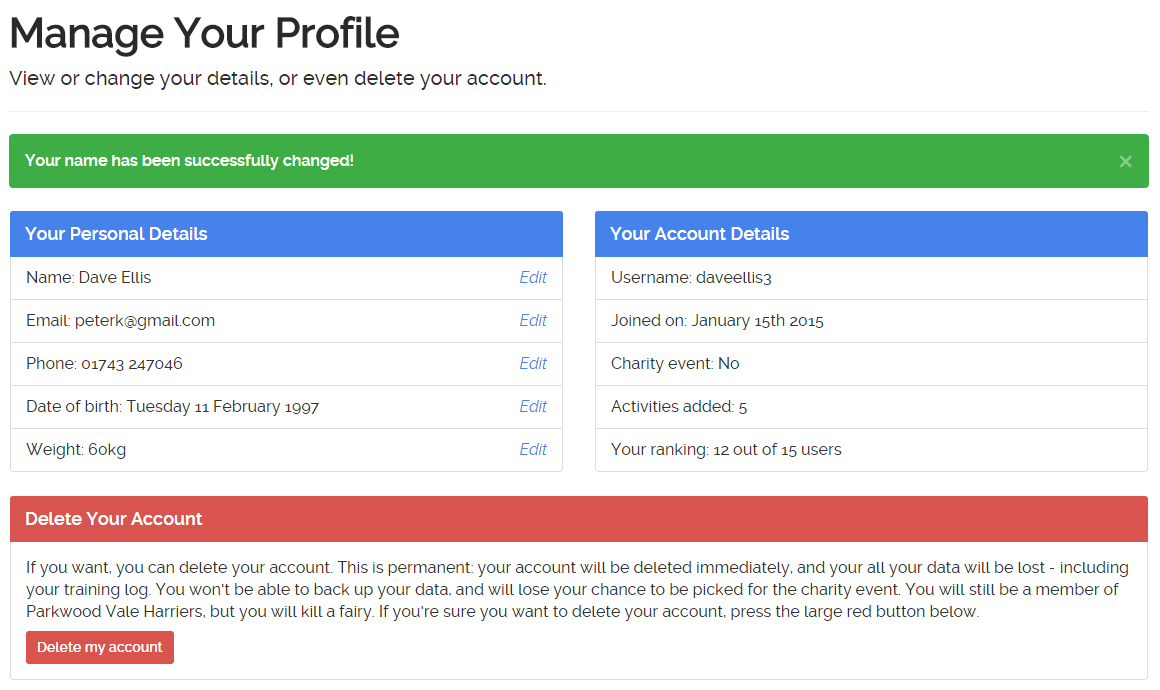
\includegraphics[scale=0.31]{images/testing/profile/change_name_success}
    \caption{Successful Name Change}
\end{figure}

\clearpage

The code is practically the same for each element that is changed, so testing one element ensures that they all work properly.

\section{Evaluation}
This is the evalulation; it evaluates different parts of the system.
\subsection{Testing Evaluation}
I believe that my testing strategy was sound: it allowed me to test most of the different parts of the system, and several bugs and flaws were fixed and sorted out through this process. Each part of the test has been well documented with clear instructions for the tester, as well as good screenshots. This has improved the quality of the system, making it more reliable for the runner.

I have tested all the validation on the system to ensure that erroneous data cannot be entered. I have tested that the database works correctly, ensuring that all read/write/update/delete operations work properly; this is a very important aspect of the system, so it is important that it works.

Additionally, I have tested the calorie calculation - it is very important that this works properly, else the incorrect team could be picked, leading to the running club performing poorly in the charity event.

Unfortunately, time restraints meant that I was unable to document the testing for the rankings page; this suggests that the testing strategy could be improved by making it quicker.

\subsection{Possible Improvements}
A major improvement would be if users were able to compare their performance, as this was unfortunately not functional at the time of release. Additionally, a seperate area for staff to view more data about the runners, and make changes of their own would be useful; it could help prevent malpractise.
 
\addcontentsline{toc}{section}{Unnumbered Section}

\end{document}